% !TeX encoding = UTF-8
% !TeX program = pdflatex
% !TeX spellcheck = en_US

\documentclass[oneside]{sapthesis}

\usepackage[procnumbered, ruled, linesnumbered]{algorithm2e}
\usepackage{amsmath}
\usepackage{amssymb}
\usepackage{balance}
\usepackage{bm}
%\usepackage[usenames,dvipsnames]{color}
%\usepackage{etoolbox}
%\usepackage{float}
\usepackage{graphicx}
\usepackage{hyperref}
\usepackage{mathtools}
\usepackage{microtype}
\usepackage{multirow}
\usepackage[normalem]{ulem}

\usepackage{cleveref}

\hypersetup{pdftitle={Generation and Control of Motion for 3D Humanoids and Steerable WMRs},pdfauthor={Michele Cipriano}}

% Commands for the titlepage
\title{Generation and Control of Motion for 3D Humanoids and Steerable WMRs}
\author{Michele Cipriano}
\IDnumber{1764645}
\course{Dottorato di Ricerca in Automatica, Bioingegneria e Ricerca Operativa - XXXVI Ciclo}
\courseorganizer{Sapienza University of Rome}
\AcademicYear{2023/2024}
\copyyear{2024}
\advisor{Prof. Giuseppe Oriolo}
%\advisor{Dr. Nome Cognome}
%\coadvisor{Dr. Nome Cognome}
\authoremail{cipriano@diag.uniroma1.it}

%\examdate{TBD May 2024}
%\examiner{Prof. TBD}
%\examiner{Prof. TBD}
%\examiner{Prof. TBD}
\versiondate{\today}

%%%%%%% Mathematical Symbols ==>>

\def\tr{^T}
\def\trd{{}^T}
\def\Atan{\mathrm{Atan2}}
\def\Acos{\mathrm{Acos}}
\def\sgn{\mathrm{sgn}}
\def\de{\mathrm{d}}
\def\diag{\mathrm{diag}}

\def\zero{\hbox{\bf 0}}
\def\Zero{{\bm{O}}}

\def\bfa{{\bm{a}}}
\def\bfb{{\bm{b}}}
\def\bfc{{\bm{c}}}
\def\bfd{{\bm{d}}}
\def\bfe{{\bm{e}}}
\def\bff{{\bm{f}}}
\def\bfg{{\bm{g}}}
\def\bfh{{\bm{h}}}
\def\bfi{{\bm{i}}}
\def\bfj{{\bm{j}}}
\def\bfk{{\bm{k}}}
\def\bfl{{\bm{l}}}
\def\bfm{{\bm{m}}}
\def\bfn{{\bm{n}}}
\def\bfo{{\bm{o}}}
\def\bfp{{\bm{p}}}
\def\bfq{{\bm{q}}}
\def\bfr{{\bm{r}}}
\def\bfs{{\bm{s}}}
\def\bft{{\bm{t}}}
\def\bfu{{\bm{u}}}
\def\bfv{{\bm{v}}}
\def\bfw{{\bm{w}}}
\def\bfx{{\bm{x}}}
\def\bfy{{\bm{y}}}
\def\bfz{{\bm{z}}}
\def\bfA{{\bm{A}}}
\def\bfB{{\bm{B}}}
\def\bfC{{\bm{C}}}
\def\bfD{{\bm{D}}}
\def\bfE{{\bm{E}}}
\def\bfF{{\bm{F}}}
\def\bfG{{\bm{G}}}
\def\bfH{{\bm{H}}}
\def\bfI{{\bm{I}}}
\def\bfJ{{\bm{J}}}
\def\bfK{{\bm{K}}}
\def\bfL{{\bm{L}}}
\def\bfM{{\bm{M}}}
\def\bfN{{\bm{N}}}
\def\bfO{{\bm{O}}}
\def\bfP{{\bm{P}}}
\def\bfQ{{\bm{Q}}}
\def\bfR{{\bm{R}}}
\def\bfS{{\bm{S}}}
\def\bfT{{\bm{T}}}
\def\bfU{{\bm{U}}}
\def\bfV{{\bm{V}}}
\def\bfW{{\bm{W}}}
\def\bfX{{\bm{X}}}
\def\bfY{{\bm{Y}}}
\def\bfZ{{\bm{Z}}}

\def\bfGamma{{\bm{\Gamma}}}
\def\bfDelta{{\bm{\Delta}}}
\def\bfTheta{{\bm{\Theta}}}
\def\bfLambda{{\bm{\Lambda}}}
\def\bfXi{{\bm{\Xi}}}
\def\bfPi{{\bm{\Pi}}}
\def\bfSigma{{\bm{\Sigma}}}
\def\bfUpsilon{{\bm{\Upsilon}}}
\def\bfPhi{{\bm{\Phi}}}
\def\bfPsi{{\bm{\Psi}}}
\def\bfOmega{{\bm{\Omega}}}
\def\bfalpha{{\bm{\alpha}}}
\def\bfbeta{{\bm{\beta}}}
\def\bfgamma{{\bm{\gamma}}}
\def\bfdelta{{\bm{\delta}}}
\def\bfepsilon{{\bm{\epsilon}}}
\def\bfzeta{{\bm{\zeta}}}
\def\bfeta{{\bm{\eta}}}
\def\bftheta{{\bm{\theta}}}
\def\bfiota{{\bm{\iota}}}
\def\bfkappa{{\bm{\kappa}}}
\def\bflambda{{\bm{\lambda}}}
\def\bfmu{{\bm{\mu}}}
\def\bfnu{{\bm{\nu}}}
\def\bfxi{{\bm{\xi}}}
\def\bfpi{{\bm{\pi}}}
\def\bfrho{{\bm{\rho}}}
\def\bfsigma{{\bm{\sigma}}}
\def\bftau{{\bm{\tau}}}
\def\bfupsilon{{\bm{\upsilon}}}
\def\bfphi{{\bm{\phi}}}
\def\bfchi{{\bm{\chi}}}
\def\bfpsi{{\bm{\psi}}}
\def\bfomega{{\bm{\omega}}}
\def\bfvarepsilon{{\bm{\varepsilon}}}
\def\bfvartheta{{\bm{\vartheta}}}
\def\bfvarpi{{\bm{\varpi}}}
\def\bfvarrho{{\bm{\varrho}}}
\def\bfvarsigma{{\bm{\varsigma}}}
\def\bfvarphi{{\bm{\varphi}}}
\def\bfimath{{\bm{\imath}}}
\def\bfjmath{{\bm{\jmath}}}


\newenvironment{braced}
 {\par\smallskip\hbox to\columnwidth\bgroup
  \hss$\left\{\begin{minipage}{\columnwidth}}
 {\end{minipage}\right.$\hss\egroup\smallskip}

\newtheorem{proposition}{Proposition}
\newtheorem{remark}{Remark}
\newtheorem{assumption}{Assumption}

\def\RealSet{{I\!\!R}}
\def\bull{\vrule height .9ex width .8ex depth -.1ex} % square bullet

\makeatletter
\newcommand{\removelatexerror}{\let\@latex@error\@gobble}
\makeatother
\let\oldnl\nl% Store \nl in \oldnl
\newcommand{\nonl}{\renewcommand{\nl}{\let\nl\oldnl}}% Remove line number for one line

\begin{document}

\frontmatter

\maketitle

%\begin{acknowledgments}
%Acknowedgments.
%\end{acknowledgments}

\begin{abstract}
Mobile robots have the potentiality to accomplish complex tasks because of 
their capability of adapting to different scenarios. This is particularly 
true for humanoid robots, which can navigate unstructured environments thanks 
to their anthropomorphic structure, and steerable wheeled mobile robots (WMRs),
which present an increased mobility with respect to their non-omnidirectional 
counterpart.

In this thesis, we focus on the problem of generation and control of motion 
for humanoid robots in 3D, and steerable WMRs. In particular, when developing 
a framework for locomotion, one should take into account how the 
robot perceives its surroundings, how to move, and how to actually perform 
the motion. These problems, which lie under the categories of perception,
motion planning, and control, must be solved efficiently and simultaneously.

In the first part of this manuscript, we study the problem of motion generation 
for humanoid robots in a world of stairs, a particular kind of uneven terrain 
where all contact surfaces are piecewise-horizontal. We present a framework 
composed of a RRT*-based footstep planner, a gait generation scheme based 
on Model Predictive Control (MPC), a mapping module, and a localization module.
The footstep planner, which plans a feasible sequence of footsteps using an
elevation map, exploits the time the robot takes to complete a step to
replan the footsteps, improving the plan and taking 
into account changes in the map, which may occur due to the presence of 
dynamic obstacles. In order to improve the reliability of locomotion,
external disturbances and pushes must be considered. To address these scenarios,
we present 
Feasibility-Aware Plan Adaptation (FAPA), a module for adapting 
footstep plans (positions, orientations, and timings) in such a way 
to guarantee the feasibility of the subsequence MPC stage. FAPA allows to 
sustain external pushes on stairs, allowing the humanoid to safely complete 
locomotion tasks.

In the second part of this manuscript, we study the problem of motion control
for steerable WMRs (SWMRs). The development of control schemes for this kind of platform 
is not trivial, due to the presence of kinematic singularities, which must 
be taken into account in order to properly make the robot move. We propose 
a framework for trajectory tracking of SWMRs using Nonlinear MPC (NMPC) based on the 
real-time iteration scheme. The NMPC generates feasible motions for the robot,
taking into account both kinematic singularities of the mobile base, and 
bounds on driving and steering velocities. Our NMPC works alongside a finite
state machine and an auxiliary trajectory generation scheme
based on dynamic feedback linearization, which makes our
framework capable of tracking trajectories without ever
encountering singularities.

The proposed methods are validated in simulation using CoppeliaSim,
and in experimental settings using the Neobotix MPO-700 platform.

\end{abstract}

\tableofcontents

\listoffigures

\mainmatter

\chapter{Introduction}
Robots are shaping our world, progressively becoming an integral part of our 
society. From manipulators in production lines, autonomous vehicles in 
space, surgical systems in hospitals to vacuum cleaners in our homes, we can 
literally say that robots are everywhere. Nevertheless, while the adoption of
autonomous systems has skyrocketed in the past few decades, and research has
made great strides, the technology of today
is not yet ready for the adoption of more complex robots, such as humanoids
and mobile manipulators.

Humanoids robots, thanks to their anthropomorphic structure, are in principle 
capable of interacting with our environment, in the same way we humans do.
One of the biggest challenges in the research of humanoids is that of 
locomotion in 3D environments, for which complex motions may be required.
Indeed, in order for humanoid robots to properly perform locomotion tasks, 
steeping over or onto obstacles, climbing and descending stairs, and 
overcoming gaps must be taken into account. 

Mobile manipulators, on the other hand, are not designed to move in such 
complex environments, but may possess the same manipulation capabilities if 
equipped with proper arms. The lower body of mobile manipulators consists
of a mobile base, which differs depending on the tasks the robot is
supposed to solve. Among the possible choices, employing a mobile base equipped 
with steerable wheels allows the robot to perform complex motions (because 
of the omnidirectionality of the base) without sacrificing its robustness
(because of the presence of classical wheels).

While, in literature, there exists a large number of methodologies for
generating and controlling the motion of mobile robots, the problems 
of locomotion of humanoids in 3D environment, and locomotion of robots 
equipped with steerable wheels (steerable wheeled mobile robots), has not been 
entirely solved yet. TODO: say the main reasons [...].

TODO: The focus of this manuscript is [...].

\section{Contribution}
Thesis contribution and list of publications.

\section{Outline}
Outline of the thesis.

\chapter{Humanoids and steerable WMRs}
\label{ch:humanoids-and-swmrs}
The idea of building a machine that replicates the human body, and is capable 
of executing the same tasks that we do, has fascinated humanity since forever.
The earliest ideas can be dated back to the third century BC, when the 
Chinese philosopher Lie Yokou described a humanoid automaton constructed of 
leather and wood, capable of moving all parts of its body
\cite{Needham1956ScienceandCivilisationinChinaVol2}. In the first century AD,
the greek mathematician and engineer Heron of Alexandria described a machine 
capable of pouring wine for party guests \cite{Alexandria2015Pneumatica}.
In 1206, the Muslim engineer Ismail al-Jazari published a book describing 
about one hundred mechanical devices, including automata performing different 
facial expressions \cite{AlJarari1206BookofKnowledge}. Among these ancient
automata, the most famous one is undoubtedly Leonardo's mechanical knight 
(or Leonardo's robot), a humanoid automaton in a suit of a knight's armor
build by Leonardo Da Vinci in 1495 \cite{Moran2006TheDaVinciRobot}.
Even though the history of robots started many centuries ago, the word ``robot''
first appears only in 1920 in the science-fiction play R.U.R.
(Rossum's Universal Robots) \cite{Capek1920RUR}, written by the Czech writer
Karel {\v C}apek.
In the last century, robots have become part of our world. Apart the adoption 
of robots in the industry, and the use of robots in academia, we are now 
used to see robots in movies (e.g., C-3PO in Star Wars,
Fig. \ref{fig:introduction:robots-in-history}), in animation (e.g., The Iron
Giant, Bender and Baymax, Fig.
\ref{fig:introduction:robots-in-animation}), and in books (Isaac Asimov
introduced the Three Laws of Robotics in his 1942 ``Runaround'' story).

This chapter gives a brief overview on the main developments in the field of 
robotics happened in the last 50 years, focusing in particular on humanoids
(from the WABOT-1 to the commercialization of humanoids)
and steerable WMRs (from interaction with humans to space exploration),
which are the type of platforms used in the following chapters.

\begin{figure}
    \centering
    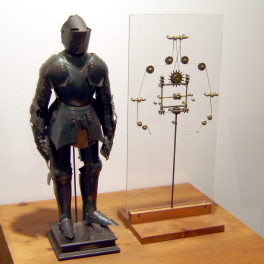
\includegraphics[width=\textwidth]{figures/01-introduction/robot-history.jpg}
    \caption{From left to right: Leonardo's robot, constructed by Leonardo Da
        Vinci in 1495 \cite{Moran2006TheDaVinciRobot};
        R.U.R. (Rossum's Universal Robots) by Karel {\v C}apek introduced 
        the word ``robot'' in 1920 \cite{Capek1920RUR};
        C-3PO, the famous humanoid robot from the Star Wars Cinematic Universe
        \cite{StarWars1977}.
    }
    \label{fig:introduction:robots-in-history}
\end{figure}

\begin{figure}
    \centering
    
\includegraphics[width=\textwidth]{figures/01-introduction/robots-in-animation.jpg}
    \caption{Humanoid robots in animation. From left to right:
        The Iron Giant (1999) \cite{TheIronGiant1999},
        Bender from Futurama (1999) \cite{Futurama1999}, and
        Baymax from Big Hero 6 (2014) \cite{BigHero62014}.
    }
    \label{fig:introduction:robots-in-animation}
\end{figure}

\subsubsection{First prototypes: WABOT-1 and WABOT-2}
The first anthropomorphic robot ever developed is the WABOT-1
\cite{Kato1973TheWABOT1}, whose project started in 1967 and completed in 1972.
The robot (Fig. \ref{fig:introduction:WABOTs}), was constituted by a limb-control
system, which allowed it to walk, and a conversation system, 
which allowed it to communicate with a person in Japanese. The development 
continued with the WABOT-2 \cite{Kato1987WABOT2}, introduced in 1984,
a musician robot able to play a keyboard instrument (Fig.
\ref{fig:introduction:WABOTs}) and read a musical score with his eyes. The WABOT
project is considered as a turning-point in the development of humanoids, as it 
introduced the first programmable multi-purpose humanoid robot.

\begin{figure}
    \centering
    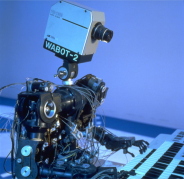
\includegraphics[width=0.7\textwidth]{figures/01-introduction/WABOTs.jpg}
    \caption{From left to right: the WABOT-1 (1972), which is the first anthropomorphic robot
        ever developed \cite{Kato1973TheWABOT1}, and the WABOT-2 (1984)
        playing a keyboard \cite{Kato1987WABOT2}.}
    \label{fig:introduction:WABOTs}
\end{figure}

\subsubsection{Honda humanoids: E series, P series and ASIMO}
During the 80s and the 90s, the development of humanoids was mainly dominated
by Honda, which introduced his first humanoid, E0, in 1986. E0 had 6 degrees
of freedom, and it could walk slowly (it needed around 5 seconds to complete 
a step) in a straight line. This model was further developed into the E-series 
robots (E1, introduced in 1987, to E6, introduced in 1993), which could walk 
faster, balance autonomously, avoid obstacles and climb stairs. The E6 was 
much heavier (150 kg) and taller (174 cm) with respect to the E0 (whose 
weight was 16.5 kg and height was 101 cm).
The development of Honda humanoids evolved into the P series. The first of these 
robots, the P1, had 30 degrees of freedom, it
was 191 cm tall and it weighed 175 kg. The P1 was kept secret until the 
announcement of the P2 in 1996, which is described in detail in
\cite{Hirai1998HondaP2}.

In 2000, Honda introduced ASIMO (Advanced Step in Innovative Mobility)
\cite{Sakagami2002ASIMO}, a humanoid robot capable of walking and running 
up to 9 km/h. Among its physical capabilities, ASIMO was able to handle trays 
and carts, and pour drinks. Moreover, because of its voice and image recognition
technologies, it was able to interact with people, giving presentations and 
providing explanations of exhibits \cite{Shigemi2019ASIMOandHumanoidRobotResearchatHonda}.
The development of ASIMO has ceased in 2018, and its last public appearence
took place in 2022.

\begin{figure}
    \centering
    \includegraphics[width=0.7\textwidth]{figures/01-introduction/The-ASIMO-humanoid-robot-history.png}
    \caption{Honda E series (E0 in 1986 to E6 in 1993) robots, Honda P series (P1 in
        1993 to P3 in 1997) robots, and ASIMO (2000)
        \cite{Shigemi2019ASIMOandHumanoidRobotResearchatHonda}.}
    \label{fig:introduction:ASIMO-humanoid-history}
\end{figure}

\subsubsection{2000s: humanoids of the new millenium}
Apart from ASIMO, the 2000s have seen the introduction of many humanoids of 
different dimension and cost, which shaped the technology of today's humanoids.
In 1998, Japan's Ministry of Economy, Trade and Industry started the Humanoid
Robotics Project (HRP), together with Kawada Industries, the National
Institute of Advanced Industrial Science and Technology (AIST) and Kawasaki
Heavy Industries, Inc. The project started with the Honda P3, which evolved 
during the decade into the HRP-2 \cite{Kaneko2004HRP2}, the HRP-3
\cite{Kaneko2008HRP3}, the HRP-4 \cite{Kaneko2011HRP4} (shown in Fig.
\ref{fig:introduction:robots-in-2000}) and the HRP-4C
\cite{Kaneko2009HRP4C}. These robots have been used in all sort of applications,
such as ladder climbing in industrial facilities \cite{Vaillant2016AuRo}, and aircraft manufacturing
\cite{Kheddar2019AircraftManufacturing}.

In 2006, the private company PAL Robotics introduced REEM-A, a humanoid designed to 
play chess, that could also walk and speak. The REEM project continued with 
the REEM-B \cite{Tellez2008REEMB}, which was introduced in 2008. The year 2006 
has seen the introduction of two other humanoids which are still used nowadays:
the NAO from Aldebaran \cite{Gouaillier2008NAOHumanoid}, used from healthcare
scenarios \cite{Cifuentes2020SocialRI} to soccer competitions \cite{Kitano1997RoboCupTR},
and the iCub \cite{Metta2010iCubHumanoid}, used mainly for research in 
cognitive robotics.

\begin{figure}
    \centering
    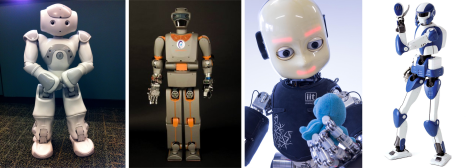
\includegraphics[width=\textwidth]{figures/01-introduction/robots-in-2000.jpg}
    \caption{Some of the humanoid robots developed in 2000s. From left to right:
        Aldebaran NAO \cite{Gouaillier2008NAOHumanoid},
        PAL Robotics REEM-B \cite{Tellez2008REEMB},
        iCub \cite{Metta2010iCubHumanoid}, and
        HRP-4 \cite{Kaneko2011HRP4}.
    }
    \label{fig:introduction:robots-in-2000}
\end{figure}

\subsubsection{2010s: DARPA robotics challenge}
The development of humanoid robots in 2010s was mainly shaped by the DARPA
Robotics Challenge \cite{Atkeson2018DARPARoboticsChallenge}, a competition 
organized by the US Defence Advanced Research Projects Agency in 2012, which 
had the objective to develop semi-autonomous humanoid robots to be deployed
in disaster scenarios. The competition consisted in solving several tasks,
such as driving a vehicle, opening a door, climbing an industrial ladder, 
using a tool to break through a concrete panel, and turn on a valve.
Amidst the robots used during the challenge, we can find the ATLAS by 
Boston Dynamics (Fig. \ref{fig:introduction:robots-in-2010}), the WALK-MAN 
developed by Italian Institute of Technology \cite{Tsagarakis2017WALKMAN},
and DRC-HUBO+ \cite{Jung2018DRCHUBO} from team KAIST, who won the challenge 
by completing all the tasks in the shortest time.

Among the other humanoid robots developed in this decade, DLR designed TORO
\cite{Englsberger2014TORO} for the study of walking and multi-contact 
balancing, NASA designed Valkyrie \cite{Radford2015Valkyrie} for advancing 
human spaceflight and extraterrestrial exploration, and PAL Robotics designed 
TALOS (Fig. \ref{fig:introduction:robots-in-2010}), a research platform mainly
targeted for industrial applications \cite{Stasse2017TALOS}.

\begin{figure}
    \centering
    \includegraphics[width=\textwidth]{figures/01-introduction/robots-in-2010.jpg}
    \caption{Some of the humanoid robots developed in 2010s. From left to right:
        Boston Dynamics ATLAS,
        WALK-MAN \cite{Tsagarakis2017WALKMAN},
        NASA Valkyrie \cite{Radford2015Valkyrie}, and
        PAL Robotics TALOS \cite{Stasse2017TALOS}.}
    \label{fig:introduction:robots-in-2010}
\end{figure}

\subsubsection{2020s: humanoid robots as commercial products}
The technology of humanoids is mature enough, and this is reflect by the 
increasing number of companies interested in building humanoid robots, and the 
large investments in robotics companies\footnote{Just to give an example,
in February 2024, Figure AI has raised \$675 million in funding, reaching 
a valuation of \$2 billion.}.

Among the humanoids currently developed by private companies, we have Digit 
by Agility Robotics (Fig. \ref{fig:introduction:robots-in-2020}), Optimus by
Tesla, Apollo by Apptronik, Figure 01 by Figure AI, NEO by 1X, Phoenix by 
Sanctuary AI, H1 by Unitree, and GR-1 by Fourier Intelligence. All these 
humanoids are being developed with one common idea in mind: they must be 
general-purpose. Indeed, the tasks they are expected to perform vary from 
moving packages in a factory, unloading trailers, palletization,
last mile delivery to automotive production, and home assistance.

In the near future, we can thus expect to see an even more rapid growth in 
humanoid robot technologies, and the introduction of humanoids in a vast 
number of industries, revolutionizing the way we work, interact,
and experience the world around us.

\begin{figure}
    \centering
    \includegraphics[width=\textwidth]{figures/01-introduction/robots-in-2020.jpg}
    \caption{Some of the humanoid robots developed in 2020s for commercial
        purposes. From left to right:
        Digit by Agility Robotics, Optimus by Tesla, Apollo by Apptronik, and
        Figure 01 by Figure AI.
    }
    \label{fig:introduction:robots-in-2020}
\end{figure}

\subsubsection{Steerable WMRs: space exploration, disaster response, human collaboration}
\begin{figure}
    \centering
    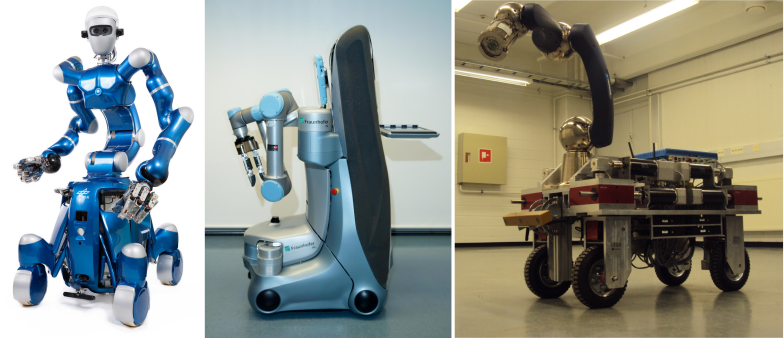
\includegraphics[width=\textwidth]{figures/01-introduction/SWMRs-1.jpg}
    \caption{Robots equipped with steerable wheels to be deployed in different areas.
        From left to right: Rollin' Justin \cite{Fuchs2009RollinJustin}, used 
        for household work and astronauts assistance in space, 
        Care-O-bot 3 \cite{Graf2009Care-O-bot3}, used as service robot, and
        iMoro \cite{Oftadeh2013iMoro}, used for inspection of contaminated
        environments.}
    \label{fig:introduction:SWMRs-1}
\end{figure}

\begin{figure}
    \centering
    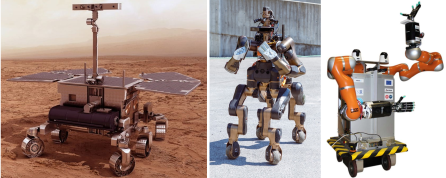
\includegraphics[width=\textwidth]{figures/01-introduction/SWMRs-2.jpg}
    \caption{More recent robots equipped with steerable wheels.
        ExoMars \cite{Poulakis2015ExoMarsMobilitySubsystem}, conceived for 
        space exploration,
        CENTAURO \cite{Kashiri2019Centauro}, designed for loco-manipulation
        in disaster scenarios, and
        BAZAR \cite{Cherubini2019ACR}, designed to interact with humans in
        assembly lines.
    }
    \label{fig:introduction:SWMRs-2}
\end{figure}

\chapter{Literature review}
\label{ch:literature-review}
In this chapter, we give an overview on the literature of locomotion for
humanoid robots and motion control for
steerable wheeled mobile robots (SWMRs). In the first part of 
the chapter, we introduce the problems of 
gait generation, footstep planning, sensor-based locomotion, and footstep and 
timing adaptation for humanoids robots. In the second part of the chapter,
we study motion control algorithms for SWMRs.

\section{Humanoid robots}
\subsection{Gait generation}
In order for humanoid robots to successfully complete their tasks, they need to 
maintain balance at all times. The problem of gait generation consists in the
generation of trajectories that keep the robot balanced, and the realization of 
such trajectories on the humanoid itself. The most common type of gaits studied for 
humanoids are \textit{walking} and \textit{running}.
In this section, we briefly review the main 
scientific contributions to the problem of walking gait generation in 
planar and 3D environments.

Humanoid walking can be \textit{static} or \textit{dynamic}. In case of planar
contacts, in static walking, the 
projection of the \textit{Center of Mass} (CoM) lies within the
\textit{support polygon},
defined as the convex hull of the contact points. In dynamic walking, 
it is the \textit{Zero-tilting Moment Point} (ZMP) \cite{Vukobratovic1972ZMP},
defined as the point 
where the moment of the contact wrench aligns with the normal of the contact 
surface \cite{SardainBessonnet2004}, which lies within the support polygon.
In case of non-coplanar contacts,
an algorithm for testing static equilibrium has been developed by Bretl in
\cite{Bretl2008TestingStaticEquilibriumforLeggedRobots}, while for dynamic
walking, a more general
condition on the ZMP has been presented by Caron in
\cite{Caron2017TRO}.

Because of the complex nonlinear dynamics of the humanoid, the problem of gait 
generation is typically decomposed into two sub-problems: trajectory generation and 
whole-body trajectory tracking. The problem of trajectory generation is 
usually solved considering a simplified dynamics, such as the \textit{Centroidal
Dynamics} (the dynamics of the humanoid projected at its CoM)
\cite{Orin2013CentroidalDynamics} or the \textit{Linear Inverted Pendulum} (LIP)
\cite{Kajita1991LIP}. The problem of trajectory tracking is solved with a 
kinematic controller, typically implemented as a
stack-of-tasks \cite{Escande2014IJRR}, and solved through a hierarchy of 
Quadratic Programming (QP) problems.

The LIP relates the CoM to the ZMP through a linear dynamics, proving a 
theoretical tool that can be used for the generation of walking gait in 
real-time \cite{Sugihara2002ICRA}. More advanced techniques for the control 
of the ZMP can be found in \cite{Kajita2003BipedWalkingPatternGeneration}, which
presents a walking pattern generation scheme using preview control, or in
\cite{Wieber2006LMPCWalking}, which develops a Linear Model Predictive Control
scheme. In particular, the latter adopted a Cart Table model
\cite{Kajita2016IntroductiontoHumanoidRobotics}, minimizing the CoM jerk while enforcing the dynamic balance
condition (ZMP within the support polygon) as a constraint. This technique
was further developed taking into account automatic footstep placement
\cite{Herdt2010OnlineWalkingMotionGenerationWithAFSP}, stability \cite{Sherikov2014Humanoids}
and recursive feasibility \cite{Ciocca2017Humanoids} of the MPC.

More recently, Scianca introduced
\textit{Intrinsically-Stable MPC} (IS-MPC) \cite{Scianca2016ISMPC, Scianca2020TRO},
a gait generation scheme which 
uses the LIP as prediction model, enforcing dynamic balance
by constraining the ZMP within the support polygon,
and using a stability constraint to ensure that the CoM does not diverge 
with respect to the ZMP \cite{Lanari2015Inversionbasedgaitgeneration}. IS-MPC,
which will be used for gait generation throughout this manuscript,
has been extended to uneven ground in \cite{Zamparelli2018SYROCO} by
considering a dynamic balance condition in 3D
\cite{Caron2017DynamicWalkingOverRoughTerrains, Sugihara2021ICRA}. Because
IS-MPC is formulated as a QP problem, it can be efficiently solved by a 
QP solver and deployed on a real robot.

\subsection{Footstep planning}
Gait generation schemes such as IS-MPC rely on \textit{footstep plans}, which specify 
how the walking should be performed at high level (where to place each footstep,
the trajectory of the swing foot, and the duration of single and double support
phases). Footstep plans can either be manually defined, or computed by a 
footstep planner. In this section we review the literature on footstep planners,
diving them in two categories. The first one will cover footstep planners 
employing continuous techniques (optimization-based),
while the second one will cover footstep planners employing discrete techniques
(deterministic and randomized approaches).

Planners based on continuous techniques compute sequences of footsteps via
optimization, treating their poses as continuous decision variables. 
Several methods in this category (e.g., \cite{Ibanez2014IROS, Hong2011TSMC,
Kasadei2021SNAS}) rely on the implicit assumption that the ground is completely
flat and, therefore, are not tailored for motion generation in 3D environments.
Explicit account of 3D environment is instead made in
\cite{Deits2014FootstepPlanningMIQCQP}: the ground surface is decomposed as a
set of convex regions (with the aid of a manual initialization phase) and
footsteps are placed by solving a mixed-integer quadratic problem (MIQP). 
A more recent work \cite{Song2021RAL} casts the MIQP into a $l_1$-minimization
problem: to reduce the computational complexity, a suboptimal solution is
found by considering only those regions that intersect with the reachable
workspace of the feet along a pre-planned trajectory for the floating base
of the robot.

Planners based on discrete techniques find a solution by searching among
particular sequences of footsteps. These sequences are generated by
concatenation of \emph{primitives}. A primitive is a displacement between two
consecutive footsteps, selected among a finite number of possible displacements
from a catalogue.

To search among all possible sequences, one possibility is to use a
deterministic approach (search-based), which is typically represented by a variant of A* \cite{Hart1968Astar}.
Chestnutt implemented the A* footstep planner in \cite{Chestnutt2005FootstepPlanningASIMO}
for the ASIMO humanoid robot \cite{Sakagami2002ASIMO}. The work has been later 
extended to adaptively extend the catalogue of primitives
\cite{Chestnutt2007AdaptiveActionModel} depending on the terrain.
Hornung implemented Weighted A* \cite{Pearl1984Heuristics},
ARA* \cite{Likhachev2003ARAstar} and R* \cite{Likhachev2008Rstar}
footstep planners with anytime 
replanning strategies in \cite{Hornung2012AnytimeSearchbasedFootstepPlanning}.
Replanning strategies using D* Lite \cite{Koenig2002Dlite} and AD*
\cite{Likhachev2005ADstar} have been respectively implemented in
\cite{Gairmort2011HumanoidNavigationwithDynamicFootstepPlans} and 
\cite{Hornung2012AdaptiveLevelofDetailPlanning}.
Although search-based algorithms have been applied to 3D environments
\cite{Griffin2019ICRA}, this kind of approach suffers from two main issues: the
performance strongly depends on the chosen heuristic, which is often difficult
to design, and node expansion can be very expensive when using a large set of
primitives, because it requires the evaluation of all possible successors.

An alternative option is to use a randomized approach (sampling-based) such as
a variants of the Rapidly-exploring Random Tree (RRT) algorithm \cite{LaValle1998RRT}. 
This has been first developed in \cite{Zeyang2009RRTFootstepPlanning,
Zeyang2011RRTFootstepPlanning} in 2D environments, and later applied in simple
3D environments \cite{Perrin2012TRO, Liu2012IROS}, showing
good performance both in planning and replanning for dynamic environments.
Recently, Ferrari \cite{Ferrari2019ECC} presented a RRT footstep planner 
for humanoid navigation in uneven terrain, which is integrated with IS-MPC.
Clearly the disadvantage of RRT over a deterministic approach is that it does
not account, at least in its basic form, for the quality of the footstep plan.

\subsection{Sensor-based locomotion}
So far, it was assumed that a complete knowledge of the environment is available
from the start, or that, in case of dynamic environment, changes to the latter
are readily communicated to the planner. However, this is not often the case in
practical situations. In fact, the environment could be unknown, either
partially or completely, and it must be reconstructed online with the aid of
on-board sensors.

Many existing methods exploit information acquired through on-board sensors to
identify planar surfaces that define safe regions where the robot can step onto
\cite{Gutmann2008EnvironmentMapGeneration, Biswas2012PlanarPolygonExtraction,
Deits2015ComputingLargeConvexRegions, Bertrand2020DetectingUsablePlanarRegions,
Mishra2021GPUAcceleratedRapidPlanarRegionExtraction}.
Such environment representation was used in combination with different kinds of
footstep planners, for example, based on simple geometric criteria
\cite{Okada2005ICRA}, A* \cite{Chestnutt2009IROS, Calvert2022BipedalWalkingoverRapidRegions}
and MIQP \cite{Fallon2015Humanoids}.   
Other methods maintain a more complete representation of the environment by
employing an elevation map \cite{Burgard2016WorldModeling}.
Examples can be found in \cite{Maier2013IROS, Stumpf2014Humanoids},
where ARA*-based approaches are used to plan footsteps on uneven ground; the
use of on-line information is aimed at improving the plan during the execution,
and not for replanning/extension using newly acquired information.
To achieve more flexibility in the on-line capabilities,
\cite{Karkowski2016Humanoids} proposed to use adaptive sets of possible foot
displacements in an A*-based planner, which proved to be effective in relatively
simple scenarios. Alternatively, \cite{Yamamoto2021AdvancedRobotics} proposed a
two-stage method that first finds a collision-free path for a bounding occupancy
volume and then computes a compatible sequence of footsteps, which is a
suitable technique as long as it is not necessary to traverse narrow passages.

\subsection{Footstep and timing adaptation}
The techniques discussed so far assume that the robot is not subject to strong 
disturbances. Nevertheless, in order for the humanoids to be deployed in
real-world scenarios, the presence of possible external forces must be taken 
into account. In principle, when subject
to external perturbations, the humanoid should be able to adapt the footstep plan
by changing the position and the timing of the footsteps.

Model Predictive Control schemes, in their basic form, allow to
perform real-time footstep position adaptation \cite{Herdt2010IROS} and obtain
reactive stepping so to reject pushes and impacts. However, in order to be
able to formulate the optimization problem as a Quadratic Program (QP),
constraints should be kept linear. For this reason, most schemes only adapt
footstep positions, leaving out footstep orientation and step timing, and not
considering the possibility to place footsteps on a different contact surface,
which is crucial when walking on uneven terrains.

Several efforts to improve this basic paradigm have been made. To include
automatic step timing adaptation, one could make the MPC nonlinear
\cite{Maximo2020MIQPAutomaticWalking,Bohorquez2017AdaptiveStepDuration,
Caron2017Whentomakeastep,Aurelien2014IROS}, denying real-time implementation or
requiring significant compromise in the control rate. A linear formulation is
obtainable by considering only the duration of the first footstep
\cite{Smaldone2021FeasibilityDrivenSTA,Khadiv2020StepTimingAdaptation}.
As for footstep orientation, this is also often ignored or planned independently
of the dynamics \cite{Herdt2010IROS}. To couple rotation decision with the
dynamics, some schemes employ non-convex optimization through nonlinear
\cite{Naveau2017RAL,Bohorquez2018AdaptiveStepRotation} or Mixed-Integer
Programming (MIP) \cite{Maximo2020MIQPAutomaticWalking}.
MIP can also be used to alternatively select between multiple convex regions
in which to place the footsteps, which would otherwise constitute a
non-convex constraint \cite{Aceituno2018RAL,Deits2014FootstepPlanningMIQCQP}.

\section{Motion control for steerable WMRs}
As already discussed in the previous chapter, mobile robots equipped with
multiple steerable wheels
have greater maneuverability than other wheeled mobile robots, since they are
omnidirectional \cite{RobuffoGiordano2009ICRA}. Besides, they can transport
higher payloads than omnidirectional robots equipped with mecanum wheels
\cite{Dickerson1991ControlOminidirectionalRobotwithMecaumWheels} or
with omni wheels \cite{Blumrich1974OmnidirectionalWheel}.
Nevertheless, modeling and controlling these robots is not
trivial due to the presence of kinematic singularities \cite{Sorour2017RAL},
which need to be handled with particular care, in order to avoid negatively
affecting their functionalities.

While many different approaches for modeling and control of steerable wheeled
mobile robots (SWMRs) exist in literature, none of them fully exploits their
potentialities. The main property of this kind of robots, indeed, is that their
instanteneous center of rotation (ICR) can be located anywhere on the plane
\cite{Campion1996TR}. This naturally leads to a parametrization based on
two-dimensional cartesian \cite{Sorour2016ICRA} or polar coordinates
\cite{Connette2008CDC}, which, however, leads to singularities that can make
it difficult to develop a control scheme. Sorour et al. \cite{Sorour2017RAL}
developed an ICR-based controller which handles singularities of the steering
axes. The work is further improved in \cite{Sorour2019RAS}, where the
singularity of the ICR at infinity is taken into account through a
complementary route strategy. While these approaches consider all singularities
of their parametrization, the velocity and acceleration bounds are only
considered at the level of the ICR, often resulting in undesired motions with
high velocity and high acceleration of the steerable wheels.
A singularity-free representation is presented in \cite{Ferland2010IROS}
and \cite{Clavien2018EstimationoftheICR}, and used in
of~\cite{Clavien2018ICRMotionControl}, where a free-of-singularity motion
controller is developed. Here, time scaling is performed to satisfy velocity
and acceleration constraints on the wheels, resulting however in
non-optimal motion execution.

\part{Motion generation for humanoid robots}
\chapter{Dynamics of humanoid locomotion}
Intro. Robot walks by exchanging forces with the environment. Dynamic balance, contacts. Simplified models and contact equilibrium.

\section{Lagrangian dynamics}
Define configuration of the robot:
\begin{equation*}
    \ddot{\bm{q}} =
    \begin{bmatrix}
        \bm{q}_b \\ \bm{q}_j
    \end{bmatrix} \in \mathrm{SE}(3) \times \mathrm{SO}(2)^{n_j}
\end{equation*}

Equations of motion
\begin{equation}
    \begin{bmatrix}
        \bm{M}_u \\ \bm{M}_a
    \end{bmatrix} \ddot{\bm{q}} +
    \begin{bmatrix}
        \bm{c}_u(\bm{q}, \dot{\bm{q}}) \\
        \bm{c}_a(\bm{q}, \dot{\bm{q}}) \\
    \end{bmatrix} =
    \begin{bmatrix}
        \bm{0} \\ \bm{\tau}
    \end{bmatrix} +
    \sum_{k=1}^{K}
    \begin{bmatrix}
        \bm{J}_{k, u}^T \\ \bm{J}_{k, a}^T
    \end{bmatrix}
    \bm{f}_k
    \label{eq:equation-of-motion-humanoids}
\end{equation}

Contact forces inside the friction cone to avoid slipping

A contact force $\bm{f}_k$ is \textit{feasible} if it lies in the friction cone $\mathcal{C}_k$ directed by the contact normal $\bm{n}_k$:
\begin{equation*}
    \| \bm{f}_k - (\bm{f}_k \cdot \bm{n}_k) \bm{n}_k \|_2 \le \mu_k (\bm{f}_k \cdot \bm{n}_k)
\end{equation*}
with $\mu_k$ static friction coefficient.

In the following we will assume that there always exists joint torques
$\bm{\tau}$ that realize the actuated part of eq.
\eqref{eq:equation-of-motion-humanoids}.

\section{Centroidal dynamics}
The above hypothesis allows as to focus on the unactuated part of the equation
\eqref{eq:equation-of-motion-humanoids}, and define the
\textit{centroidal dynamics} \cite{Orin2013CentroidalDynamics} of the humanoid
\begin{equation}
    \label{eq:centroidal-dynamics}
    \begin{bmatrix}
        m \ddot{\bm{p}}_C \\ \dot{\bm{L}}_C
    \end{bmatrix} =
    \begin{bmatrix}
        m \bm{g} \\ \bm{0}
    \end{bmatrix} +
    \sum_{k=1}^k
    \begin{bmatrix}
        \bm{f}_k \\ (\bm{p}_C - \bm{p}_k) \times \bm{f}_k
    \end{bmatrix}
\end{equation}
where $m$ is the total mass of the robot, $\bm{p}_C$ is the position of its
center of mass (CoM),
$\bm{g} = (0, 0, -g)^T$ is the gravity vector, $\bm{f}_k$ is the contact force
applied at point with coordinates $\bm{p}_k$ over a contact surface with normal
$\bm{n}_k$, $K$ is the total number of contacts, and $\bm{L}_c$ is the angular
momentum of the robot taken at the CoM.

Let us define the \textit{gravito-inertial wrench} taken at point $O$ as
\begin{equation}
    \label{eq:gravito-intertial-wrench}
    \bm{w}_O^{\rm gi}
    =
    \begin{bmatrix}
        \bm{f}^{\rm gi}\\
        \bm{\tau}_O^{\rm gi}
    \end{bmatrix}
    =
    \begin{bmatrix}
        m \bm{g} - m \bm{\ddot{p}}_C \\
        (\bm{p}_C - \bm{p}_O) \times (m \bm{g} - m \bm{\ddot{p}}_C) - \bm{\dot{L}}_C
    \end{bmatrix}
\end{equation}

\section{Zero-tilting moment point}
\label{sec:zero-tilting-moment-point}
Consider the gravito-inertial wrench defined in \ref{eq:gravito-intertial-wrench}. Zero-tilting moment points (ZMPs) are points $Z$ where the moment of the contact wrench aligns with the normal $\bm{n}$ of the contact surface \cite{SardainBessonnet2004}, i.e.,
\begin{equation}
    \label{eq:zmp-non-tilting-condition}
    \bm{\tau}_Z^{\rm gi} \times \bm{n} = \bm{0}
\end{equation}
which, using Varignon formula\footnote{A screw $\bm{w}_O =
(\bm{f},\bm{\tau}_O)$ represents the generalized force acting on a rigid body
\cite{Featherstone2007RigidBodyDynamicsAlgorithms},
and it is composed by a linear force $\bm{f}$ passing through $O$, together with the
total moment $\bm{\tau}_O$ about $O$. That total moment around any other point
$A$ can be computed using Varignon formula as $\bm{\tau}_A=\bm{\tau}_O+\bm{f}\times(\bm{p}_A-\bm{p}_O)$.}, can be rewritten as
\begin{equation}
    \left(\bm{\tau}_O^{\rm gi} + (\bm{p}_O - \bm{p}_Z) \times \bm{f}^{\rm gi}\right) \times \bm{n} = \bm{0}
\end{equation}
which, developing the triple cross product\footnote{The triple cross product
between three vectors $\bm{a}, \bm{b}, \bm{c} \in \mathrm{R}^n$ is defined as
the cross product of the vector $\bm{a}$ with the cross product of the other
two: $\bm{a}\times(\bm{b}\times\bm{c})=(\bm{a}\cdot\bm{c})\bm{b}-
(\bm{a}\cdot\bm{b})\bm{c}$. Note that, since the cross product is anticommutative,
the following holds:
($\bm{a}\times\bm{b})\times\bm{c}=-(\bm{c}\cdot\bm{b})\bm{a}+
(\bm{c}\cdot\bm{a})\bm{b}$.}, becomes
\begin{equation}
    \bm{\tau}_O^{\rm gi} \times \bm{n} - (\bm{n} \cdot \bm{f}^{\rm gi}) (\bm{p}_O - \bm{p}_Z) - \left(\bm{n} \cdot (\bm{p}_O - \bm{p}_Z)\right) \bm{f}^{\rm gi} = \bm{0}
\end{equation}

Assuming that point $Z$ lies on a plane with normal $\bm{n}$ intersecting the point $O$, i.e. $Z \in \Pi(O, n)$, the term $\bm{n} \cdot (\bm{p}_O - \bm{p}_Z) = 0$, and the above equation can be easily rewritten as
\begin{equation}
    \bm{p}_Z = \bm{p}_O + \frac{\bm{n} \times \bm{\tau}_O^{\rm gi}}{\bm{n} \cdot \bm{f}^{\rm gi}}
\end{equation}
finally defining the ZMP $Z$. Notice that, more in general, there exists an infinity of ZMPs which lie on the non-central axis defined by \eqref{eq:zmp-non-tilting-condition}. For more details, please refer to \cite{SardainBessonnet2004}.

\subsection{Relationship between CoM, ZMP and angular momentum}
Consider the non-tilting condition of Eq. \eqref{eq:zmp-non-tilting-condition}. Using Varignon formula $\bm{\tau}_Z^{\rm gi} = \bm{\tau}_C^{\rm gi} + \bm{f}^{\rm gi} \times (\bm{p}_Z - \bm{p}_C)$, we have that
\begin{equation}
    \left(\bm{\tau}_C^{\rm gi} + \bm{f}^{\rm gi} \times (\bm{p}_Z - \bm{p}_C)\right) \times \bm{n} = \bm{0}
\end{equation}
which, computing the triple product, becomes
\begin{equation}
    \bm{\tau}_C^{\rm gi} \times \bm{n} - \left(\bm{n} \cdot (\bm{p}_Z - \bm{p}_C)\right) \bm{g}^{\rm gi} + (\bm{n} \cdot \bm{f}^{\rm gi}) (\bm{p}_Z - \bm{p}_C) = \bm{0}
\end{equation}

Applying the definition of \textit{gravito-inertial wrench} of Eq. \eqref{eq:gravito-intertial-wrench} and rearranging the terms, it is simple to prove \cite{Caron2017TRO} the following relationship between the CoM acceleration, the ZMP position and the angular momentum:
\begin{equation}
    \label{eq:relationship-com-zmp-angular-momentum}
    \ddot{\bm{p}}_C = \bm{g} + \frac{\bm{n} \cdot (\bm{\ddot{p}}_C - \bm{g})}{\bm{n} \cdot (\bm{p}_C - \bm{p}_Z)} (\bm{p}_C - \bm{p}_Z) + \frac{\bm{n} \times \bm{\dot{L}}_C}{m \left(\bm{n} \cdot (\bm{p}_C - \bm{p}_Z)\right)}
\end{equation}
\section{3D LIPM}
The centroidal dynamics \eqref{eq:centroidal-dynamics} is, in general,
nonlinear, due to variations of angular momentum and height of the CoM. In this
section, we derive the dynamics of the 3D Linear Inverted Pendulum
\cite{Kajita2016IntroductiontoHumanoidRobotics}. To do so, we assume that the
rate of change of angular momentum is negligible (i.e., $\dot{\bm{L}}_C = 0$),
and constrain the vertical motion of the CoM so that
\begin{equation}
    \frac{\ddot{z}_C + g}{z_C - z_Z} =
    \frac{\bm{n} \cdot (\ddot{\bm{p}}_C - \bm{g})}{\bm{n} \cdot (\bm{p}_C - \bm{p}_Z)} =
    \eta^2,
\end{equation}
with $\eta$ an arbitrary constant \cite{Zamparelli2018SYROCO}. In this way,
the relationship \eqref{eq:relationship-com-zmp-angular-momentum} becomes
\begin{equation}
    \ddot{\bm{p}}_C = \eta^2 (\bm{p}_C - \bm{p}_Z) + \bm{g},
\end{equation}
which corresponds to the 3D LIPM (Linear Inverted Pendulum Mode).

\section{Contact equilibrium}
Todo (describe pyramid in SYROCO18, which is a particular case of the 3D LIPM).

\chapter{Gait generation via IS-MPC}
\section{Gait generation via IS-MPC (from WoS)}
\label{sec:WoS:offlineCase:GaitGeneration}
The gait generation module receives the planned footstep sequence ${\cal S}_f$ as input, and it is in charge of producing a CoM trajectory that the robot can safely track in order to step over said footstep sequence. Along the entire motion, dynamic balance must be maintained.

On flat ground, it is common to ensure dynamic balance as a geometric criterion, by requiring that the ZMP must always be inside the convex hull of contact surfaces, i.e., the \emph{support polygon}. Traditionally, the ZMP is assumed to be located on the ground plane, which is uniquely defined when the environment is flat.

In non-flat environments, there is no unique ground surface on which the ZMP can be assumed to be. However, the aforementioned criterion can be extended to these cases by allowing the ZMP to move in 3D \cite{SuImYaCa:2021}. The balance criterion is satisfied as long as the ZMP is inside a three-dimensional \emph{support region} $\mathcal{Z}$ that takes the shape of a pyramid (see Fig.~\ref{fig:WoS:balance3d}). The vertex of this pyramid is the robot CoM, and the edges are the lines connecting the CoM to the vertexes of the convex hull of the contact surfaces.

In MPC, dynamic balance is enforced via constraints on the ZMP position. However, the 3D support region $\mathcal{Z}$ cannot be directly employed to enforce a ZMP constraint, because this would be nonlinear, meaning that the resulting optimization problem would not be in a standard linear-quadratic formulation. The cause of this nonlinearity is given by the fact that the vertex of the pyramid $\mathcal{Z}$ is the CoM. Since both the ZMP and the CoM depend on the decision variables of the QP, this would result in product between the decision variables themselves.

In order to avoid this, we will define a smaller region, independent of the CoM position, where the ZMP is allowed to be. Furthermore, we will prove that this region conservatively approximates the actual support region $\mathcal{Z}$, and thus that the balance condition is always satisfied under the imposed constraints.

In this section we will describe the MPC gait generation scheme that is used in the proposed formulation. In particular, we will derive the prediction model and define the constraints that ensure stability and dynamic balance. Finally, we will state the QP problem to be solved at each iteration, and give a sketch of the complete algorithm.

\smallskip

\subsection{Prediction Model}

Control of the ZMP is achieved using a dynamic model relating the position of the latter to the position and acceleration of the CoM. This dynamic model can be derived by balancing moments on the humanoid as a whole, and assuming that the rate of change of angular momentum around the CoM can be neglected. With this in mind, denoting the CoM as $\bfp_c = (x_c, y_c, z_c)$ and the ZMP as $\bfp_z = (x_z, y_z, z_z)$, we get
\begin{equation}\begin{split}
(z_c - z_z)\ddot x_c &= (x_c - x_z)(\ddot z_c - g) \\
(z_c - z_z)\ddot y_c &= (y_c - y_z)(\ddot z_c - g),
\end{split}\end{equation}
where $g$ is the gravity acceleration.

This model exhibits a nonlinear coupling between the vertical and the horizontal components of $\bfp_c$ and $\ddot\bfp_c$. On flat ground, this nonlinearity is usually handled by assuming a constant CoM height, which leads to the well-known LIP model~\cite{KaKaKaFuHaYoHi:03}. In order to allow for vertical movement of the CoM, a different choice is made here, which is to constrain the motion of the CoM to satisfy the relation $(\ddot z_c - g)/(z_c - z_z) = \eta^2$, where $\eta$ is a constant parameter.
The resulting dynamic model can be expressed in the form
\begin{equation}\label{eq:WoS:3dmodel}
\ddot \bfp_c = \eta^2(\bfp_c - \bfp_z) - \bfg,
\end{equation}
where $\bfg = (0\,\,\,0\,\,\,g)^T$ is the gravity acceleration vector. This model features a LIP-like dynamic behavior along all three axes. The only difference with respect to a standard LIP is given by the gravity vector $\bfg$ acting as a constant drift. This causes the system not to be in equilibrium when the CoM and ZMP coincide, but rather when they are displaced by $\bfg/\eta^2$.

The choice of restricting the available trajectories to those resulting in a constant $\eta$ allows to make the prediction model linear. If this restriction is removed, the model is referred to as Variable-Height Inverted Pendulum, which can be treated either as nonlinear or time-varying. This can allow for more general motions to be generated, e.g., running~\cite{Smaldone2022Running}, at the cost of a slightly more complex architecture. For the present case, where only walking is considered, the simpler model is preferred.

In order to obtain smoother trajectories, model (\ref{eq:WoS:3dmodel}) is dynamically extended to have the derivative of the ZMP $\dot \bfp_z$ as the input.
The gait generation scheme works over discrete time-steps of duration $\delta$, over which the input $\dot \bfp_z$ is assumed to be constant, i.e., $\dot \bfp_z(t) = \dot \bfp_z^k$ for $t\in[t_k, t_{k+1})$.
This prediction model is used to forecast the evolution of the system over a receding horizon window called the \emph{control horizon}, spanning a time $T_c=C\delta$. The number of steps that are contained, either fully or partially, within this control horizon is denoted as $F$.

\smallskip

\subsection{Stability Constraint}

Model~(\ref{eq:WoS:3dmodel}) has a positive eigenvalue $\eta$, reflecting the intrinsic instability of the humanoid dynamics. Given this instability, it is not sufficient to generate a gait such that the ZMP is inside the support region, because the associated CoM trajectory might be divergent, making the motion unrealizable by the humanoid.
The role of the stability constraint is to enforce a condition on the unstable component of the dynamics in order to guarantee that the CoM trajectory does not diverge with respect to the ZMP.

The unstable component of system (\ref{eq:WoS:3dmodel}) is highlighted by the coordinate $\bfp_u = \bfp_c + \dot \bfp_c/\eta$,
also referred to as Divergent Component of Motion (DCM) or Capture Point (CP), that evolves according to the dynamics
\begin{equation}
\dot\bfp_u = \eta(\bfp_u - \bfp_z) - \frac{\bfg}{\eta}.
\end{equation}
Despite the instability, the evolution of the system is bounded if the following \emph{stability condition} is satisfied
\begin{equation}
\label{eq:WoS:stabilitycondition}
\bfp_u^k = \eta\int_{t_k}^{\infty}e^{-\eta(\tau - t_k)}\bfp_z(\tau) d\tau + \frac{\bfg}{\eta^2},
\end{equation}
as stated by the following proposition.

\medskip

\begin{proposition}
Consider system~(\ref{eq:WoS:3dmodel}). If the ZMP velocity is bounded, 
$|\dot x_z|\le v^{\rm max}$, $|\dot y_z|\le v^{\rm max}$, $|\dot z_z|\le v^{\rm max}$, for some $v^{\rm max}>0$, and condition~(\ref{eq:WoS:stabilitycondition}) is satisfied, then the following bound holds:
\begin{equation}
\label{eq:WoS:ZMPbound}
\frac{\bfg}{\eta^2}- \frac{v^{\rm max}}{\eta}{\bf 1} \le \bfp_c-\bfp_z \le \frac{\bfg}{\eta^2}+\frac{v^{\rm max}}{\eta}{\bf 1},
\end{equation}
where ${\bf 1}$ is a vector with all components equal to 1. Moreover, (\ref{eq:WoS:ZMPbound}) implies that the system is internally stable, i.e., the CoM is bounded with respect to the ZMP.
\label{prop:velocityBound}
\end{proposition}

\medskip

\emph{Proof}. See Appendix.

\medskip

Condition~(\ref{eq:WoS:stabilitycondition}) is non-causal as it requires knowledge of the future ZMP trajectory $\bfp_z$ up to infinity. In order to derive a causal implementation, we split the integral at $t_{k+C}$. Of the two separate integrals that result, the first, over $[t_k, t_{k+C})$, can be expressed in terms of the MPC decision variables. A value for the second integral, over $[t_{k+C}, \infty)$, can be obtained by conjecturing a ZMP trajectory using information coming from the footstep plan.
This conjectured trajectory is called \emph{anticipative tail} and is denoted with $\tilde \bfx_z$. 
In \cite{ScDeLaOr:20}, the anticipative tail was used to prove recursive feasibility and stability of the MPC scheme.

The stability constraint is then written as
\begin{equation}\label{eq:WoS:stability_constraint}
\eta\int_{t_k}^{t_{k+C}}e^{-\eta(\tau - t_k)}\bfp_z d\tau = \bfp_u^k - \tilde \bfc^k - \frac{\bfg}{\eta^2}.
\end{equation}
where $\tilde \bfc^k$ is given by
\begin{equation}%\label{eq:WoS:stability_constraint}
\tilde\bfc^k = \eta\int_{t_{k+C}}^{\infty}e^{-\eta(\tau - t_k)}\tilde\bfp_z d\tau.
\end{equation}

Note that in \cite{ScDeLaOr:20} we considered the footstep plan to be available over a receding window called the \emph{preview horizon}. Here there is no need to make such an assumption, as the footstep plan is provided in its entirety, and once the goal is reached the robot comes to a complete stop.

Enforcing constraint (\ref{eq:WoS:stability_constraint}) allows, similarly to what stated in Prop.~\ref{prop:velocityBound}, to bound the displacement between CoM and ZMP. In fact, the value of the bound is almost identical in most practical situation, especially in view of the fact that the preview horizon is unlimited because the plan is completely known. Because of this fact, we will assume in the following that Prop.~\ref{prop:velocityBound} is valid as stated, even though a small numerical correction should be applied to make up for the difference between the stability condition and the stability constraint.



\smallskip

\subsection{ZMP Velocity Constraint}

This constraint imposes a limit on how fast the ZMP can move, i.e.,
\begin{equation}\label{eq:WoS:ZMP_velocity_constraint}
|\dot x_z|\le v^{\rm max}, \quad |\dot y_z|\le v^{\rm max}, \quad |\dot z_z|\le v^{\rm max}
\end{equation}
Enforcing such limit allows to indirectly control the maximum CoM/ZMP displacement, by using the result of Prop.~\ref{prop:velocityBound}. This will be useful when defining the ZMP position constraint, as will be made clear in the following paragraphs.

\smallskip

\subsection{ZMP Position Constraint}
As already noted, the humanoid is balanced as long as the ZMP is inside the pyramid $\cal Z$, which is a nonlinear condition due to the vertex of the pyramid being at the CoM (Fig. \ref{fig:WoS:balance3d}). To preserve linearity we consider a smaller allowed region for the ZMP, consisting in a box of fixed size with changing center and orientation. We refer to this as the {\em moving box}\footnote{Approximating the pyramidal region $\cal Z$ with a box might seem overly conservative. However, we argue that the neglected portion of the pyramid region is not crucial here, because large displacements of the ZMP in the $z$ direction would only be required to generate large vertical accelerations, which are not necessary in the considered setting (walking in a world of stairs). Clearly, less conservative approximations can still be envisaged and used for generating more dynamic motions.}, and we will prove that it conservatively approximates the support region, meaning that it is always contained inside the pyramid $\cal Z$.



%However, we argue that the neglected portion of the pyramid region is not crucial here, because large displacements of the ZMP in the $z$ direction are only required to generate large vertical accelerations, which are not necessary in the considered setting (walking in a world of stairs).



\begin{figure}
    \centering
    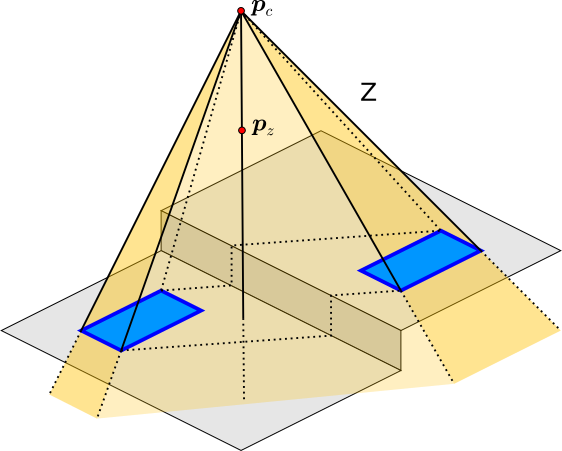
\includegraphics[width=0.6\textwidth]{figures/balance3d.pdf}
    \caption{Balance condition in 3D: the ZMP must lie inside the yellow pyramid.}
    \label{fig:WoS:balance3d}
\end{figure}

\begin{figure}
    \centering
    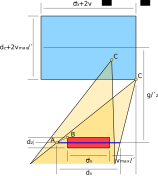
\includegraphics[width=0.6\textwidth]{figures/conservative.pdf}
    \caption{The red rectangle represents a section of the moving box in the $x$-$z$ plane. This region is fully contained inside the yellow pyramid as long as the CoM belongs to the blue region. Here, two scenarios are considered: one in which the CoM is well within the blue region, and a worst-case scenario in which the CoM is in a lower vertex of the blue region.}
    \label{fig:WoS:conservative}
\end{figure}

The center $\bfp_{\rm mc}$ and orientation $\theta_{\rm mc}$ of the moving box are taken to be consistent with the pose of footstep $\bff^j$ during the $j$-th single support phase. In the following double support phase they will gradually slide in order to reach the pose of the next footstep $\bff^{j+1}$, with a linear\footnote{The timing law can be arbitrarily chosen as long as it leads the moving box from one footstep to the next within the duration of the double support phase.} timing law. At each time $t$, the center of the moving box $\bfp_{\rm mc}$ is expressed as
\begin{equation}\label{eq:WoS: moving constraint}
\bfp_{\rm mc}(t) = \Bigg\{
\begin{array}{ll}
\bfp^j & t\in [t_s^j, t_s^j + T_{\rm ss}^j) \\
(1-\alpha^j(t))\bfp^j + \alpha^j(t)\bfp^{j+1} & t\in [t_s^j + T_{\rm ss}^j, t_s^{k+1})
\end{array}
\end{equation}
where $j=0,\dots,F$ is a index over the footsteps within the control horizon, and $\alpha^j(t) = (t-t_s^j-T_{\rm ss}^j)/T_{\rm ds}^j$ denotes the time elapsed since the start of the double support phase, expressed as a fraction of the duration of the double support phase itself.
The orientation of the moving box $\theta_{\rm mc}$ can be similarly expressed as
\begin{equation}\label{eq:WoS: moving constraint angle}
\theta_{\rm mc}(t) = \Bigg\{
\begin{array}{ll}
\theta^j & t\in [t_s^j, t_s^j + T_{\rm ss}^j) \\
\mathrm{anglin}(\theta^j,\theta^{j+1},\alpha^j(t)) & t\in [t_s^j + T_{\rm ss}^j, t_s^{k+1})
\end{array}
\end{equation}
where $j=0,\dots,F$, and $\mathrm{anglin}$ is a function\footnote{For two generic angles
$\theta_a$ and $\theta_b$, linearly combined with a weight $\alpha$, the function $\mathrm{anglin}$ can be defined as
\begin{equation*}\begin{split}
\mathrm{anglin}(\theta_a, \theta_b, \alpha) = \mathrm{atan2}(&\sin((1-\alpha)\theta_a) + \sin(\alpha\theta_b), \\&\cos((1-\alpha)\theta_a) + \cos(\alpha\theta_b)).
\end{split}\end{equation*}
Note that this definition is meaningless when the two angles are separated by exactly $\pi$, but this can never occur as the angle between consecutive footsteps is limited by requirement R2. } that computes a linear combination of angles in such a way to correctly account for wrapping around $\pm\pi$.

The ZMP position constraint is expressed as
\begin{equation}\label{eq:WoS:ZMP_constraint}
-\tilde\bfd /2 \le \bfR_{k+i}^T(\bfp_z^{k+i} - \bfp_{\rm mc}^{k+i}) \le \tilde\bfd /2
\end{equation}
where $\bfp_z^{k+i}$ and $\bfp_{\rm mc}^{k+i}$ respectively denote the ZMP and the center of the moving box sampled at time $t_{k+i}$, $\tilde \bfd = (\tilde d_x, \tilde d_y, d_z)^T$
is a vector collecting the dimensions of the moving box along all three axes, and $\bfR_{k+i}$ is the rotation matrix associated with $\theta_{\rm mc}^{k+i}$.

The size of the moving box $\tilde \bfd = (\tilde d_x, \tilde d_y, d_z)^T$ is determined in such a way to always be contained inside the pyramid $\cal Z$, as expressed by the following proposition.

\medskip

\begin{proposition}
Assume the stability constraint~(\ref{eq:WoS:stability_constraint}) and the ZMP velocity constraint~(\ref{eq:WoS:ZMP_velocity_constraint}) are enforced. If $v^{\rm max}$ is chosen in such a way that
\begin{equation}
v^{\rm max} \le \min \{v_y^{\rm max},v_x^{\rm max}\},
\end{equation}
where $v_x^{\rm max}$ and $v_y^{\rm max}$ are given by the following compact expression
\begin{equation}\label{eq:WoS:conservative_condition}
v_{x,y}^{\rm max} = \eta\left(g/\eta^2 - d_{x,y}\frac{d_z}{d_{x,y} - \tilde d_{x,y}}\right)\left(1 + \frac{d_z}{d_{x,y} - \tilde d_{x,y}}\right)^{-1},
\end{equation}
with $d_x$ and $d_y$ denoting the size of the actual footprint, then the moving box is always contained in the pyramid $\cal Z$.
\label{prop:conservative-box}
\end{proposition}

\medskip

{\em Proof}: Consider the geometric construction in Fig.~\ref{fig:WoS:conservative}. This construction shows a projection of the pyramid ${\cal Z}$ in the $x$-$z$ plane during a single support phase. The red area represents a cross section of the moving box, with dimensions $\tilde d_x$ and $d_z$. The blue area represents the region where the CoM can be found, given the CoM/ZMP bounds~(\ref{eq:WoS:ZMPbound}). In the figure two different possibilities are depicted for the CoM position (identified by the point $C$). Among them, consider the worst-case scenario, in which the CoM is in the bottom-right corner of the blue region\footnote{An equivalent symmetrical scenario would occur if the CoM were in the bottom-left corner. }. A condition for which the red region is always fully contained inside $\cal Z$ can be found by imposing that the slope of the segment $AB$ is less than the slope of the segment $AC$, i.e.,
\begin{equation}
\frac{d_z/2}{d_x/2 - \tilde d_x/2} \le \frac{g/\eta^2 - d_z/2 - v^{\rm max}_x/\eta}{d_x/2 + \tilde d_x/2 + v^{\rm max}_x/\eta},
\end{equation}
which, after simple manipulations, leads to (\ref{eq:WoS:conservative_condition}). During double support phases the construction of Fig.~\ref{fig:WoS:conservative} is not accurate anymore, as the pyramid $\mathcal{Z}$ is much larger than the one represented. However, it is not necessary to repeat the reasoning, as a smaller pyramid, analogous to that shown in Fig.~\ref{fig:WoS:conservative}, can always be constructed and will always be contained inside $\mathcal{Z}$. The last step is to repeat the construction in the $y$-$z$ plane in order to find $v_y^{\rm max}$, which proves the thesis.
\hfill\bull
\smallskip
\subsection{QP Problem}
At a generic time $t_k$, IS-MPC solves the following QP problem

\smallskip

\begin{braced}
\[
\min_{\dot \bfp_z^k, \dots, \dot \bfp_z^{k+C-1}} \quad \sum_{i=0}^{C-1} \left(\|\dot\bfp_z^{k+i}\|^2 + \beta\|\bfp_z^{k+i} - \bfp_{\rm mc}^{k+i}\|^2\right)
\]
\hspace{0.25cm} subject to:
\begin{itemize}
\item stability constraint (\ref{eq:WoS:stability_constraint})
\item ZMP velocity constraint (\ref{eq:WoS:ZMP_velocity_constraint})
\item ZMP position constraint (\ref{eq:WoS:ZMP_constraint})
\end{itemize}
\end{braced}
\smallskip
The cost function minimizes the decision variables (ZMP derivative) as a regularization term, and attempts to bring the ZMP close to the center of the moving box, which is typically beneficial as it produces a more robust walking pattern. $\beta$ is a weight on the second term.

In typical MPC fashion, the first sample of the ZMP velocity $\dot \bfp_z^k$ is used to integrate the 3D LIP dynamics (\ref{eq:WoS:3dmodel}). The resulting CoM trajectory $\bfp_c$ is sent, together with the swing foot trajectory generated by the footstep planner and sampled at time $t_k$, to the kinematic controller.

\subsection{Proof of Prop. \ref{prop:velocityBound}}
\label{sec:WoS:Proof}

Starting from the initial condition $\bfp_u(t_k)$ described by (\ref{eq:WoS:stabilitycondition}), the unstable coordinate $\bfp_u$ evolves as
\begin{equation}
\label{eq:WoS:bounded_evolution}
\bfp_u(t) = \eta\int_{t}^\infty e^{-\eta(\tau-t)}\bfp_z(\tau) d\tau + \frac{\bfg}{\eta^2}.
\end{equation}
Integrating \ref{eq:WoS:bounded_evolution} by parts gives
\begin{equation}
\label{eq:WoS:bounded_evolution_integrated}
\bfp_u(t) - \bfp_z(t) - \frac{\bfg}{\eta^2} = \int_{t}^\infty e^{-\eta(\tau-t)}\dot\bfp_z d\tau.
\end{equation}
Since by hypothesis the ZMP velocity $\dot\bfp_z$ is component-wise bounded, i.e., $|\dot x_z| \le v^{\rm max}$, $|\dot y_z| \le v^{\rm max}$, $|\dot z_z| \le v^{\rm max}$, then the following upper bound is obtained
\begin{equation*}
\bfp_u(t) - \bfp_z(t) - \frac{\bfg}{\eta^2} \leq v^{\rm max}{\bf 1}\int_{t}^\infty e^{-\eta(\tau-t)}  d\tau,
\end{equation*}
along with a similar lower bound.
%Since the ZMP velocity constraint is enforced, the components of $\dot\bfp_z$ are bounded by $|\dot x_z| \le v_{\rm max}$, $|\dot y_z| \le v_{\rm max}$, $|\dot z_z| \le v_{\rm max}$. Thus, by evaluating the integral, we obtain
The two bounds can be combined in the following expression
\begin{equation}
\label{eq:WoS:bound unstable}
-\frac{v^{\rm max}}{\eta}{\bf 1}
\le
\bfp_u(t) - \bfp_z(t) - \frac{\bfg}{\eta^2}
\le
\frac{v^{\rm max}}{\eta}{\bf 1}.
\end{equation}

Define now the coordinate $\bfp_s = \bfp_c - \dot \bfp_c/\eta$. This coordinate pertains to the stable eigenvalue of system (\ref{eq:WoS:3dmodel}), and its dynamics can be expressed as
\begin{equation*}
\dot\bfp_s = \eta(-\bfp_s + \bfp_z) + \frac{\bfg}{\eta}.
\end{equation*}
Starting from an initial time $t_0$, the coordinate $\bfp_s$ evolves as
\begin{equation*}
\bfp_s(t) = \bfp_s(t_0) e^{-\eta(t-t_0)} + \eta\int_{t_0}^t e^{-\eta(t-\tau)}\left(\bfp_z(\tau)  +\frac{\bfg}{\eta^2}\right)d\tau.
\end{equation*}
Similarly to $\bfp_u$, the above expression can manipulated using integration by parts, and the resulting integral can be bounded using the hypothesis on the ZMP velocity. The resulting expression is
\begin{equation*}
-\frac{v^{\rm max}}{\eta}{\bf 1} + \bfs_0
\le
\bfp_s(t) - \bfp_z(t) - \frac{\bfg}{\eta^2}
\le
\frac{v^{\rm max}}{\eta}{\bf 1} + \bfs_0,
\end{equation*}
where $\bfs_0 = \bfp_s(t_0) - \bfp_z(t_0) - \bfg/\eta^2$. 
Since at $t_0$ the robot is typically in static equilibrium, corresponding to $\bfp_c(t_0) = \bfp_z(t_0) + \bfg/\eta^2$ and $\dot{\bfp}_c(t_0) = 0$, then $\bfs_0 = 0$. This leads to
\begin{equation}
-\frac{v^{\rm max}}{\eta}{\bf 1}\label{eq:WoS:bound stable}
\le
\bfp_s(t) - \bfp_z(t) - \frac{\bfg}{\eta^2}
\le
\frac{v^{\rm max}}{\eta}{\bf 1}.
\end{equation}
By noting that $2\bfp_c = \bfp_u + \bfp_s$, combining eqs. (\ref{eq:WoS:bound unstable}) and (\ref{eq:WoS:bound stable}) proves the thesis.

\chapter{Humanoid motion generation in a world of stairs}

% Define and set new counter for environment procedure:
\newcounter{procedure}
\makeatletter
\AtBeginEnvironment{procedure}{\let\c@algocf\c@procedure}
\makeatother



\makeatletter
\newcommand{\removelatexerror}{\let\@latex@error\@gobble}
\makeatother
\let\oldnl\nl% Store \nl in \oldnl
\newcommand{\nonl}{\renewcommand{\nl}{\let\nl\oldnl}}% Remove line number for one line

\renewcommand\textfraction{0.0}
\renewcommand\bottomfraction{1.0}
\renewcommand\topfraction{1.0}
\renewcommand\dbltopfraction{1.0}
\setcounter{topnumber}{8}
\setcounter{dbltopnumber}{8}
\setcounter{bottomnumber}{8}
\setcounter{totalnumber}{8}

% macros
\def\RealSet{{I\!\!R}}
\def\bull{\vrule height .9ex width .8ex depth -.1ex} % square bullet
\newtheorem{proposition}{Proposition}
\newtheorem{remark}{Remark}
\newtheorem{assumption}{Assumption}

\newenvironment{braced}
 {\par\smallskip\hbox to\columnwidth\bgroup
  \hss$\left\{\begin{minipage}{\columnwidth}}
 {\end{minipage}\right.$\hss\egroup\smallskip}

	
	%%%%%%%%%%%%%%%%%%%%%%%%
	%%%%% ABSTRACT %%%%%%%%%
	%%%%%%%%%%%%%%%%%%%%%%%%
	
%\begin{abstract} 
%Consider the problem of generating humanoid motions in an environment consisting of horizontal patches located at different heights ({\em world of stairs}).
%To this end, the paper proposes an integrated scheme which combines footstep planning and gait generation. 
%In particular, footsteps are produced by a randomized algorithm that guarantees both feasibility and quality of the plan according to a chosen criterion; whereas for 3D gait generation we devise an ad hoc extension of the Intrinsically Stable MPC scheme. 
%In its basic form, the proposed scheme addresses the off-line case (known environments), but a sensor-based adaptation is developed for the on-line case (unknown environments) based on an anytime version of the footstep planner.
%In order to validate the proposed approach, we present simulations in CoppeliaSim for the HRP-4 humanoid robot navigating scenarios of different complexity, both in the on-line and off-line case.
%\end{abstract}

\section{Introduction} 
\label{sec:WoS:Introduction}

Humanoid robots, thanks to their ability to perform legged locomotion, are in principle capable of moving through 3D environments, for which complex motions might be required. These can include stepping over or onto obstacles, climbing and descending stairs, moving through surfaces located at different height, overcoming gaps, and so on.

Walking on uneven ground, however, is a challenging task. Management of the footstep locations is subject to several constraints that are completely absent in flat ground locomotion, such as the necessity to avoid placing the feet over the edge of a stair step, or determining whether a given feature of the environment should be considered useful surface onto which the robot can step or simply regarded as an obstacle and avoided altogether.

Also from a control standpoint, walking on uneven ground introduces complications in the dynamic model that are not present in flat ground locomotion. In fact, traditional humanoid locomotion is realized by approximating the dynamics using linear models, which are relatively accurate in many application. Straight up extending these models to 3D environments can lead, without additional considerations, to nonlinearities which can severely impact the performance and theoretical guarantees of the controller.

In this paper we consider the problem of generating a humanoid motion in a \textit{world of stairs}, a specific kind of uneven ground consisting of horizontal patches located at different heights. In order to successfully achieve this, it is necessary to plan a footstep sequence and a whole body motion for the humanoid realizing such sequence. We choose to approach the problem by keeping these two stages separate. The reason for this choice is that in this way we can better control the quality of the produced motions. In fact, the quality of the footstep plan can be evaluated based on global requirements, such as the number of steps taken, or a different performance index. As for the quality of the motion itself, this should be mainly addressed by its capability to satisfy all the required constraints, in order to avoid falls and instabilities. Maintaining a separation between planning and control also greatly simplifies the tuning because the domain in which any given parameter has effect is reduced.

Keeping planning and control separated is relatively straightforward when the planning is done off-line. However, it might be more difficult to realize if one wants to allow for on-line planning and replanning. In this paper, we will discuss an on-line architecture that achieves this by having short planning stages interleaved with the motion, in such a way that the planning can fully utilize sensor information gathered by the robot as it moves, and that the robot itself can take advantage of the on-line planner to find more efficient and safe footstep sequences.

In the following, we present a review of the state-of-the-art by separating the literature that is more focused on the planning aspect from the literature about gait generation and humanoid robot control. Subsequently, we will describe the contributions of the paper, focusing on the improvements with respect to the state-of-the-art.

\subsection{Contribution and paper organization}

In this paper, we consider planning both in off-line situations, in which the environment is completely known, and on-line situations, in which the geometry of the environment is not known in advance and must be reconstructed by the robot itself during motion using on-board sensors. In this case, planning and execution are interdependent: the former clearly requires the latter in order to determine where to place the footsteps, but the converse is also true, as the real-time motion of the robot is necessary to acquire information about the environment.

With respect to the previously reviewed contributions, our work improves the following points:

\begin{itemize}
\item the proposed footstep planner finds sequences of footsteps that are optimal with respect to a chosen optimality criterion, whereas most of the literature that makes use of randomized methods does not in any way consider the quality of the produced sequences \cite{Liu_IROS2012}; we do this by using a planner based on RRT*, which is a probabilistic method with guarantees of asymptotic convergence to an optimal solution;

\item in our formulation, optimality does not significantly compromise performance, unlike techniques that make use of A*-based algorithms \cite{Chestnutt_IROS2009,Maier_IROS2013,Karkowski_HUM2016}, or others that make use of quadratic optimization \cite{DeTe:14};

\item we propose a scheme capable of working both with off-line planning, in known environments, and in on-line situations;


\item to generate a gait that realizes the footstep plan we adopt and improve our Intrinsically Stable MPC (IS-MPC) scheme \cite{ScDeLaOr:20}. IS-MPC incorporates an explicit stability constraint in order to deal with the instability in the humanoid robot dynamics. Along with the stability constraint, we enforce a ZMP position constraint and a ZMP velocity constraint, and show that the combination of all the imposed constraints guarantees satisfaction of the balance condition in 3D.

\end{itemize}


Compared to our previous work on the subject, \cite{FeScLaOr:19}, the main additions presented in this paper consist of the introduction of optimality criteria in the planner, the extension to on-line situations with the use of on-board sensors, and the inclusion of the ZMP velocity constraint in the IS-MPC. We validate the proposed architectures for the off-line and on-line case via simulations on the HRP-4 humanoid robot in scenarios of different complexity.


The paper is structured as follows. Section~\ref{sec:WoS:Formulation} formulates the problem both in the off-line and in the on-line case. Section~\ref{sec:WoS:offlineCase} presents in detail the off-line case by discussing its general architecture in Sect.~\ref{sec:WoS:offlineCase:GeneralArchitecture}, describing the footstep planner and the scenarios used for testing in Sect.~\ref{sec:WoS:offlineCase:FootstepPlanner}, the gait generation module together with theoretical developments in Sect.~\ref{sec:WoS:offlineCase:GaitGeneration}, the localization module in Sect.~\ref{sec:WoS:offlineCase:Localization} and the simulations in Sect. \ref{sec:WoS:offlineCase:Simulations}. Section~\ref{sec:WoS:onlineCase} extends the work to the on-line case, presenting its architecture in Sect.~\ref{sec:WoS:onlineCase:GeneralArchitecture}, the mapping module in Sect.~\ref{sec:WoS:onlineCase:MappingModule}, the sensor-based footstep planner in Sect.~\ref{sec:WoS:onlineCase:FootstepPlanner}, the visual task generation module in Sect.~\ref{sec:WoS:onlineCase:VisualTaskGeneration} and simulations in both static and dynamic environments in Sect. \ref{sec:WoS:onlineCase:Simulations}. Section~\ref{sec:WoS:discussion} puts the paper in perspective with respect to the state of the art, and Sect.~\ref{sec:WoS:Conclusions} concludes the paper with mentions to possible future work.

	
\section{Problem formulation}
\label{sec:WoS:Formulation}


\begin{figure}
\centering
\includegraphics[width=0.9\textwidth]{figures/WoS_Scenario.PNG}
\caption{An instance of the considered problem. The robot must reach the goal region (in yellow) by traversing a {\em world of stairs}. Patches that are not visible correspond to infinitely deep holes or trenches.}
\label{fig:WoS:WoSScenario}
\end{figure}

\begin{figure}
\centering
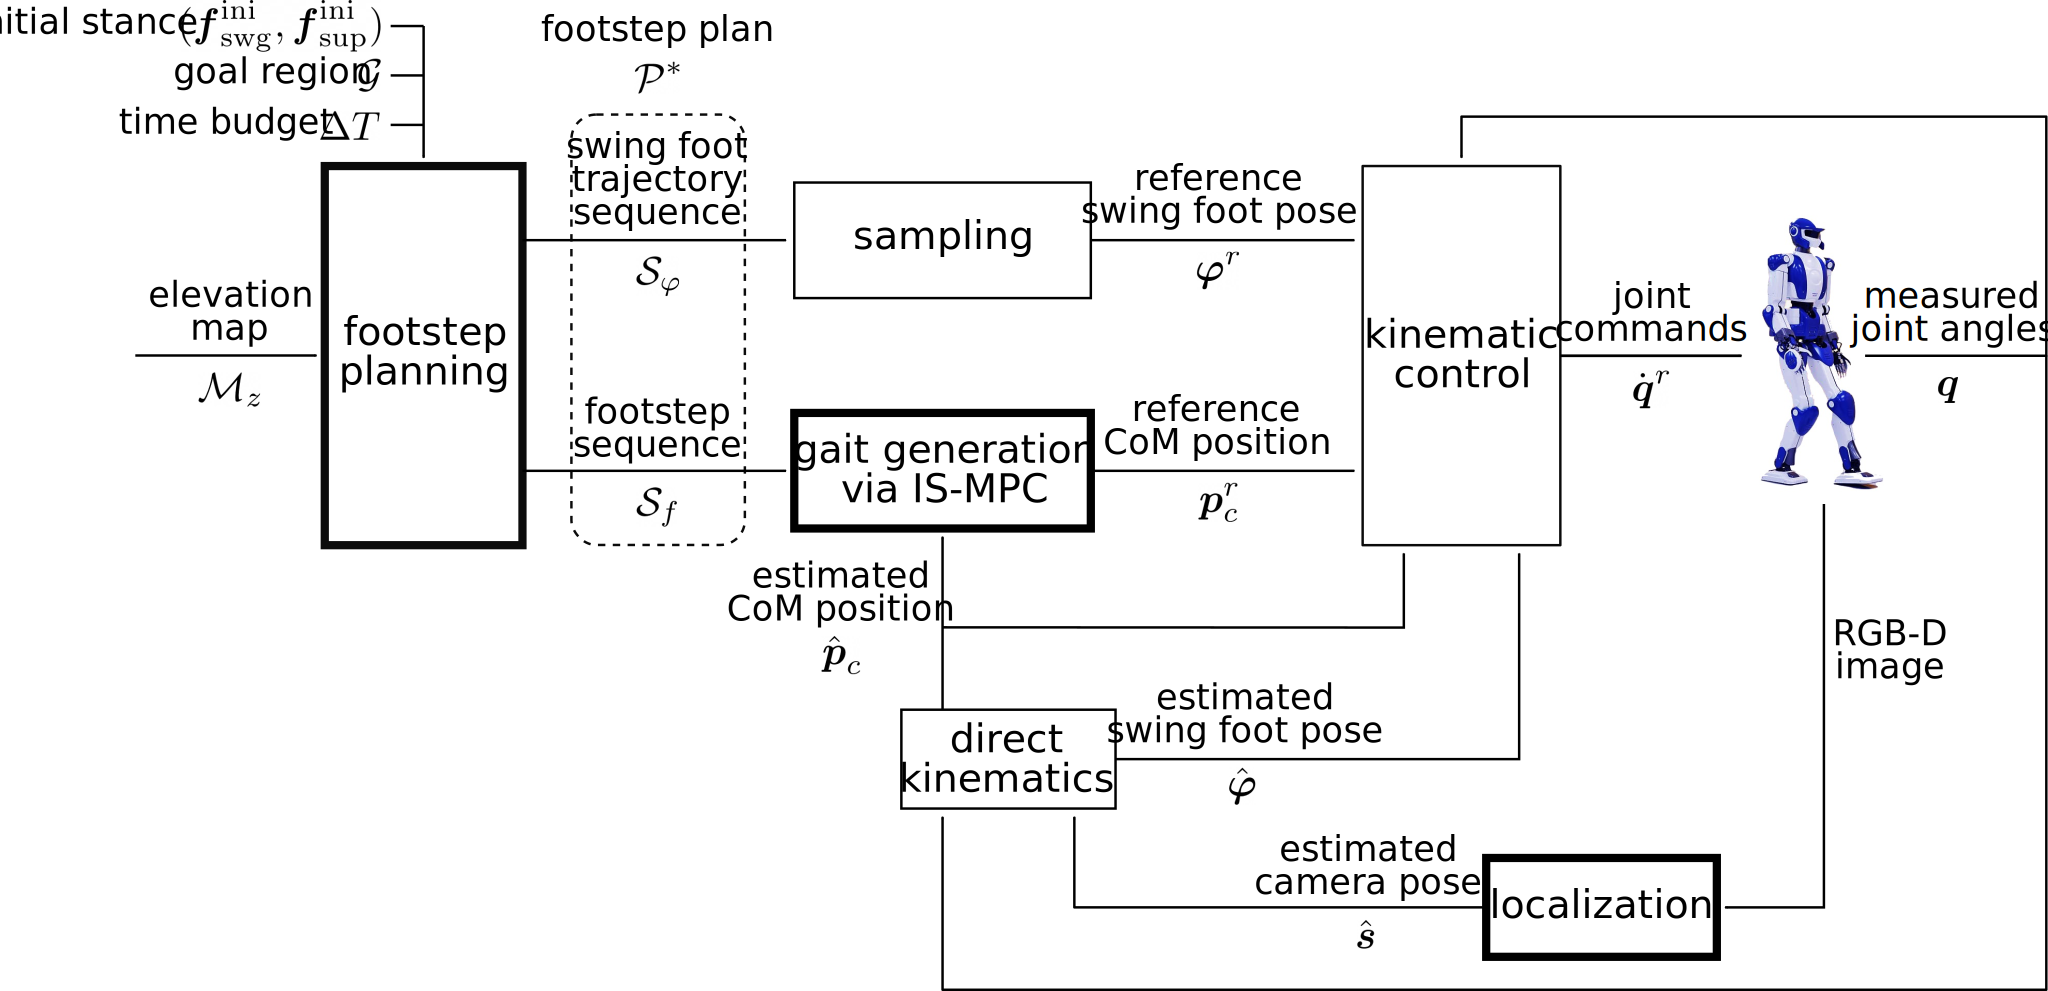
\includegraphics[width=\textwidth]{figures/BlockSchemeOffline.pdf}
\caption{Block scheme of the proposed solution approach for the off-line case.}
\label{fig:WoS:blockScheme1}
\end{figure}

In the situation of interest (Fig.~\ref{fig:WoS:WoSScenario}), a humanoid robot moves in a {\em world of stairs}, a specific kind of uneven ground consisting of horizontal patches that {\em (i)} are located at different heights, and {\em (ii)} constitute a partition\footnote{This implies that the whole volume of space below any horizontal patch is occupied.} of $\RealSet^2$. 
Depending on its elevation with respect to the neighboring areas, a patch may be accessible for the humanoid to climb on from an appropriate direction; otherwise, it actually represents an {\em obstacle} to be avoided. Any accessible patch may be stepped on, stepped over or even circumvented, depending on the generated motion.  

The mission of the robot is to reach a certain goal region $\cal G$, which will belong in general to a single patch (Fig.~ \ref{fig:WoS:WoSScenario}). In particular, this locomotion task is accomplished as soon as the robot places a footstep inside $\cal G$.

We want to devise a complete framework enabling the humanoid to plan and execute a motion to fulfill the assigned task in the world of stairs.
This requires addressing two fundamental problems: finding a 3D footstep plan and generating a variable-height gait that is consistent with such plan.
Footstep planning consists in finding both footstep placements and swing foot trajectories between them; overall, the footstep plan must be feasible (in a sense to be formally defined later) for the humanoid, given the characteristics of the environment. Gait generation consists in finding a CoM trajectory which realizes the footstep plan while guaranteeing dynamic balance of the robot at all time instants. From the trajectories of the CoM and the feet, a whole-body motion may be computed using inverse kinematics methods.

In particular, we will address two versions of the above problem, henceforth referred to as the \textit{off-line} and \textit{on-line} case. In the first, the geometry of the environment is completely known in advance, while in the second it is reconstructed by the robot itself as it moves. 
%In both cases, it is assumed that the environment is static.
%, while the on-line case naturally lends itself to the inclusion of moving obstacles.   
%is naturally tailored for unknown environments.
In the following we describe the architectures designed for the off-line and on-line case supposing that the environment is static.
%under the assumption that the environment is static. 
However, we will also show that the latter can be used effectively in dynamic environments, thanks to its fast replanning capabilities. 
%The result section will include some simulations in this sense.

The problem will be solved under the following assumptions.

\begin{itemize}

\item[A1] Information about the environment is maintained in an {\em elevation map} ${\cal M}_{z}$, i.e., a 2.5D grid map of equally-sized cells that, whenever needed, can be queried as $z = {\cal M}_{z}(x,y)$, to provide the height of the ground at the cell having coordinates $(x,y)$ \cite{BuHeBe:16}.
In the off-line case, ${\cal M}_{z}$ is available a priori, while in the on-line case it must be incrementally built by the humanoid based on sensory information. 
    
\item[A2] The humanoid is equipped with a head-mounted RGB-D camera, which is used for localization in both the off-line and on-line cases, and also updating the elevation map ${\cal M}_{z}$ in the latter.
    
\item[A3] The humanoid is endowed with a localization module which provides an estimate of the camera pose at each time instant, based on information gathered by the RGB-D camera. This is used in both the off-line and on-line cases.

\item[A4] The friction between the robot feet and the ground is sufficiently large to avoid slipping at the contact surfaces\footnote{Since our objective is to generate walking gaits in a world of stairs, we expect that the horizontal components of the ground reaction forces will be rather limited with respect to the vertical components, making this assumption reasonable. To support this claim, we explicitly verified that Assumption A4 holds in our simulations, see the related comment toward the end of Sect.~\ref{sec:WoS:offlineCase:Simulations}. Nevertheless, the constraint that ground reaction forces must always be contained in the friction cone can be incorporated in our formulation; this extension would be required in the case of non-horizontal contact surfaces.}.

\end{itemize}

In the off-line case, a complete footstep plan leading to the goal region $\cal G$ will be computed before the humanoid starts to move. In the on-line case, the footstep plan will instead be updated during motion, based on new information added to ${\cal M}_{z}$. 

In the following, we first address in full detail the off-line case and then proceed to extending the proposed approach to the on-line case.

\section{The off-line case} 
\label{sec:WoS:offlineCase}

We start this section by describing the general structure of the proposed method. Then we will describe in detail its main components, i.e., the footstep planner and the gait generation scheme based on IS-MPC. Some simulation results will also be presented.   

\subsection{General architecture}
\label{sec:WoS:offlineCase:GeneralArchitecture}

To solve the described problem in the off-line case, we adopt the architecture shown in Fig.~\ref{fig:WoS:blockScheme1}, in which the main components are the footstep planning, gait generation and localization modules.

In the following, we denote by $\bff = (x_{f}, y_{f}, z_{f}, \theta_{f})$ the {\em pose} of a certain footstep, with $x_{f}$, $y_{f}$, $z_{f}$ representing the coordinates of a representative point, henceforth collectively denoted as $\bfp_f$, and $\theta_{f}$ its orientation\footnote{To represent the footstep orientation we only use the yaw angle, as roll and pitch are always zero thanks to the piecewise-horizontal ground assumption.}.
Moreover, a pair $(\bff_{\rm swg}, \bff_{\rm sup})$ defines a {\em stance}, i.e., the feet poses during a double support phase after which a step is performed by moving the swing foot from $\bff_{\rm swg}$ while keeping the support foot at $\bff_{\rm sup}$. 

The footstep planner receives in input the initial humanoid stance\footnote{The initial support foot can be chosen arbitrarily.} $(\bff_{\rm swg}^{\rm ini}, \bff_{\rm sup}^{\rm ini})$ at $t=0$, the goal region $\cal G$, a time budget $\Delta T$, and the elevation map ${\cal M}_z$ representing the environment.

The time budget represents the time given to the planner to find a solution. When this time runs over, the algorithm either returns a solution or ends with a failure. Explicitly specifying this time as input to the algorithm allows us to evaluate the performance of the planning module, but also proves to be useful for the extension to the on-line case, where the time budget is set equal to the duration of a step in order to meet the real-time requirement.

The planner works off-line to find, within $\Delta T$, an optimal \textit{footstep plan} ${\cal P}^\ast = \{ {\cal S}_f, {\cal S}_\varphi \}$ leading to the desired goal region $\cal G$. In ${\cal P}^*$, we denote by
\begin{equation*}
    {\cal S}_f = \{\bff^1, \dots, \bff^n\}
\end{equation*}
the sequence of footstep placements, whose generic element $\bff^j$ is the pose of the $j$-th footstep, with $\bff^1 = \bff_{\rm swg}^{\rm ini}$ and $\bff^2 = \bff_{\rm sup}^{\rm ini}$. Also, we denote by
\begin{equation*}
    {\cal S}_\varphi = \{\bfvarphi^1, \dots, \bfvarphi^{n-2}\}
\end{equation*} 
the sequence of associated swing foot trajectories, whose generic element $\bfvarphi^j$ is the $j$-th {\em step}, i.e., the trajectory leading the foot from $\bff^{j}$ to $\bff^{j+2}$. Its duration $T_s^j$ is split in $T_{\rm ss}^j$ and $T_{\rm ds}^j$, respectively the single and double support phases. 
The timestamp of a generic footstep indicates the beginning of the $j$-th step, i.e., of the $j$-th single support phase; thus, $\bff^{j}$ has an associated timestamp $t_s^{j} = t_s^{j-1} + T_s^{j-1}$, with $t_s^{1}=0$.

Once the footstep plan has been generated, the sequence of footsteps ${\cal S}_{f}$ is sent to a gait generator based on Intrinsically Stable MPC (IS-MPC), which computes in real time a variable-height CoM trajectory that is compatible with ${\cal S}_{f}$ and guaranteed to be {\em stable} (i.e., bounded with respect to the ZMP). In particular, we denote by $\bfp_{\rm c}^r$ the current reference position of the CoM produced by IS-MPC. Also, let $\bfvarphi^r$ be the current reference pose of the swing foot, obtained by sampling the appropriate subtrajectory in ${\cal S}_{\varphi}$. Then, $\bfp_{\rm c}^r$ and $\bfvarphi^r$ are passed to a kinematic controller which computes the joint commands $\dot{\bfq}^r$ for the robot.

Visual information, gathered by the head-mounted camera in the form of RGB-D images, is provided to the localization module, which continuously updates the estimate $\hat{\bfs}$ of the pose of the camera frame.
From this, and using joint encoder data, it is possible to obtain estimates for the CoM position and swing foot pose ($\hat \bfp_c$ and $\hat \bfvarphi$, respectively) through kinematic computations. Finally, these estimates are used to provide feedback to both the gait generation and kinematic control modules.

\subsection{Footstep planning}
\label{sec:WoS:offlineCase:FootstepPlanner}

The input data for this module are the initial robot stance $(\bff_{\rm swg}^{\rm ini}, \bff_{\rm sup}^{\rm ini})$, the goal region $\cal G$, the time budget $\Delta T$ and the elevation map ${\cal M}_z$. Given an optimality criterion, the footstep planner returns the best footstep plan ${\cal P}^*$ leading to $\cal G$ found within $\Delta T$. 

The planning algorithm builds a tree $\cal T$, where each vertex $v = (\bff_{\rm swg}, \bff_{\rm sup})$ specifies a stance, and an edge between two vertexes $v$ and $v' = (\bff'_{\rm swg}\!=\!\bff_{\rm sup}, \bff'_{\rm sup})$ indicates a step between the two stances, i.e., a collision-free trajectory such that one foot swings from $\bff_{\rm swg}$ to $\bff'_{\rm sup}$ and the other is fixed at $\bff_{\rm sup}$.

The expansion process makes use of a catalogue $U$ of {\em primitives}, which allows to generate new footsteps by selecting them from a finite set of displacements with respect to the support foot. The catalogue is split in two subsets, one for the case of left support  and the other for the case of right support; at each instant, the appropriate subset is used. An example catalogue is shown in Fig.~\ref{fig:WoS:Primitives}.

\begin{figure}
\centering
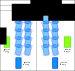
\includegraphics[width=0.65\textwidth]{figures/Primitives.pdf}
\caption{An example catalogue $U$ of primitives, containing a finite set of landings for the swing foot with respect to the left or right support foot.}
%The figure refers to the case of left support; the catalogue for right support is specular. When generating a candidate vertex, the support foot is placed at $\bff_{\rm sup}^{\rm near}$ and the chosen primitive will be taken as $\bff_{\rm sup}^{\rm cand}$.}
\label{fig:WoS:Primitives}
\end{figure}

Each branch joining the root of the tree to a generic vertex $v$ represents a footstep plan $\cal P$. The sequences ${\cal S}_f$ and ${\cal S}_\varphi$ for this plan are respectively obtained by taking along the branch the support foot poses of all vertexes and the steps corresponding to all edges.

\medskip

\subsubsection{Footstep feasibility}

Footstep $\bff^j=(x_f^j,y_f^j,z_f^j,\theta_f^j) \in {\cal S}_f$ is \textit{feasible} if it satisfies the following requirements:   

\begin{itemize}

\smallskip
\item[R1] $\bff^j$ is fully in contact within a single horizontal patch.

\smallskip
To guarantee this, each cell of ${\cal M}_{z}$ belonging to, or overlapping with, the footprint at $\bff^j$ must have the same height $z_{f}^j$. In practice, one typically uses an enlarged footprint to ensure that this requirement will still be satisfied in the presence of small positioning errors.

\smallskip
% this is actually stance feasibility 
\item[R2] $\bff^j$ is kinematically admissible from the previous footstep $\bff^{j-1}$ (this is actually {\em stance feasibility}).

\smallskip
%The admissible region (a submanifold of $\RealSet^3 \times SO(2)$) for placing $\bff^{j}$ next to $\bff^{j-1}$ is denoted by ${\cal A}(\bff^{j-1})$ and is defined by the following constraints:
The admissible region (a submanifold of $\RealSet^3 \times SO(2)$) for placing $\bff^{j}$ next to $\bff^{j-1}$ is defined by the following constraints:
\begin{gather} 
-\begin{pmatrix}
\Delta_x^- \\[5pt] \Delta_y^-
\end{pmatrix}
\le
R_{j-1}^T \begin{pmatrix}
x_f^j - x_f^{j-1} \\[5pt] y_f^j - y_f^{j-1}
\end{pmatrix}
\pm \begin{pmatrix}
0 \\ \ell
\end{pmatrix}
\le
\begin{pmatrix}
\Delta_x^+ \\[5pt] \Delta_y^+
\end{pmatrix} \label{eq:WoS:XYAdmissible}\\[5pt]
-\Delta_z^- \le z_f^j - z_f^{j-1} \le \Delta_z^+
\label{eq:WoS:ZAdmissible}\\[5pt]
-\Delta_\theta^- \le \theta_f^j - \theta_f^{j-1} \le \Delta_\theta^+. \label{eq:WoS:ThetaAdmissible}
\end{gather}
Here, $R_{j-1}$ is the planar rotation matrix associated with $\theta_f^{j-1}$ and the $\Delta$ symbols are lower and upper maximum increments, see Fig.~\ref{fig:WoS:KinCon}.

\begin{figure}
\centering
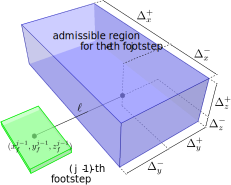
\includegraphics[width=0.6\textwidth]{figures/kinematic_limits.png}
\caption{The 3D admissible region identified by the first two kinematic constraints of requirement R2, i.e., eqs. (\ref{eq:WoS:XYAdmissible}-- \ref{eq:WoS:ZAdmissible}). Footstep orientation is not represented.}
\label{fig:WoS:KinCon}
\end{figure}

% this is actually step feasibility, i.e., compatibility between successive stances
\smallskip
\item[R3] $\bff^j$ is reachable from $\bff^{j-2}$ through a collision-free motion (this is actually {\em step feasibility}).

\smallskip
Since information about the whole-body motion of the robot is not yet available during footstep planning (it will only be defined in the subsequent gait generation phase), this requirement can only be tested conservatively. In particular, we say that R3 is satisfied if ({\em i}) there exist a collision-free swing foot trajectory $\bfvarphi^{j-2}$ from $\bff^{j-2}$ to $\bff^{j}$ generated by the engine of Sect.~\ref{sec:WoS:offlineCase:FP:PlannerOverview}, and ({\em ii}) a suitable volume ${\cal B}$ accounting for the maximum occupancy of the humanoid upper body at stance $(\bff^{j-1}, \bff^{j})$ is collision-free. More precisely, ${\cal B}$ is a vertical cylinder whose base has radius $r_b$ and center at $(x_m, y_m, z_m + z_b)$, where $x_m$, $y_m$, $z_m$ are the coordinates of the midpoint $\bfm$ between the footsteps and $z_b$ is a vertical offset representing the average distance between the ground and the hip (Fig. \ref{fig:WoS:ReqCollisionCheck}). 
Note that any nonzero height can be used for the cylinder in view of the world of stairs assumption, which implies that ${\cal B}$ is collision-free \footnote{Even though the volume for checking the upper body collision is chosen conservatively, this does not guarantee obstacle avoidance because the lower body is not considered. However, whole-body collision avoidance can be obtained by including appropriate constraints in the kinematic controller \cite{Escande_SoT2014}.} if each cell of ${\cal M}_z$ belonging to, or overlapping with, its ground projection has height smaller than $z_m + z_b$.

\end{itemize}

\medskip

\subsubsection{Vertex identity, neighbors and cost}
\label{sec:WoS:offlineCase:FP:CostFunctions}
The {\em identity} of a vertex $v=(\bff_{\rm swg}, \bff_{\rm sup})$ indicates whether  $\bff_{\rm swg}$ refers to the left ($L$) or the right ($R$) foot:
\[
{\rm id}(v)=
\begin{cases}
L\quad \mbox{if} \quad{\rm id}(v^{\rm parent}) = R \\
R\quad \mbox{if} \quad{\rm id}(v^{\rm parent}) = L,
\end{cases}
\]
where $v^{\rm parent}$ is the parent vertex of $v$.
This definition determines the identity of each vertex, once the identity of the root is assigned.

We also define the set of {\em neighbors} of $v=(\bff_{\rm swg}, \bff_{\rm sup})$
\[
{\cal N}(v) = \{ v'=(\bff'_{\rm swg}, \bff'_{\rm sup}) \in {\cal T} : 
 \gamma(\bff_{\rm sup}, \bff'_{\rm sup}) \le r_{\rm neigh}\}
\]
where $r_{\rm neigh}$ is a threshold distance and
\begin{equation}
\gamma(\bff, \bff') = \lVert \bfp_f - \bfp_f' \rVert + k_{\gamma}|\theta_f-\theta_f'|
\label{eq:WoS:footstepToFootstepMetric}
\end{equation}
is a footstep-to-footstep metric, with $k_{\gamma}\ge 0$.

\begin{figure}
\centering
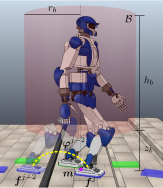
\includegraphics[width=0.55\textwidth]{figures/R3_CollisionCheck.png}
\caption{Visual representation of the process for checking requirement R3. The red cylinder accounts for the maximum occupancy of the humanoid upper body, while the yellow line represents the swing foot trajectory.}
\label{fig:WoS:ReqCollisionCheck}
\end{figure}

Assume that the edge between two vertexes $v^a$ and $v^b$ of $\cal T$ has a cost $l(v^a,v^b)$. 
The {\em cost} of a vertex $v$ is defined as
\[
c(v) = c(v^{\rm parent}) + l(v^{\rm parent}, v)
\]
and represents the cost of reaching $v$ from the root of $\cal T$. 
Then, the cost of a plan $\cal P$ ending at a vertex $v$ is $c({\cal P}) = c(v)$.

In particular, we will consider three possibilities for the cost of an edge. The first is
\begin{equation}
l_1(v^a, v^b) = 1,
\label{eq:WoS:costSteps}
\end{equation}
for all edges in $\cal T$. The corresponding vertex cost will be denoted by $c_1(v)$ and represents the length of the corresponding plan in terms of number of edges (i.e., steps). 
    
\begin{figure}
\centering
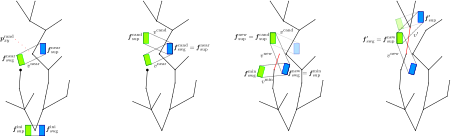
\includegraphics[width=\textwidth]{figures/FootstepPlanner.pdf}
\caption{The four steps of a generic iteration of the footstep planner. From left to right: selecting a vertex for expansion, generating a candidate vertex, choosing a parent, rewiring.}
\label{fig:WoS:FootstepPlanner}
\end{figure}   
    
The second edge cost represents the net height variation of the swing foot during a step:
\begin{equation}
l_2(v^a, v^b) = |z^b_{f, {\rm sup}} - z^a_{f, {\rm swg}}|,
\label{eq:WoS:costHeight}
\end{equation}
where $z^a_{f, {\rm swg}}$ and $z^b_{f, {\rm sup}}$ are the $z$-component of, respectively, the swing foot at $v^a$ and the support foot at $v^b$.  The corresponding vertex cost will be denoted by $c_2(v)$ and represents the cumulative height variation along the corresponding plan. 
    
Finally, we  also consider as edge cost
\begin{equation}
l_3(v^a, v^b) = \frac{1}{\sigma (\bff^b_{\rm sup})},
\label{eq:WoS:costClearance}
\end{equation}
where $\sigma (\bff^b_{\rm sup})$ is the {\em clearance} of the support foot $\bff^b_{\rm sup}$ at $v^b$, defined as the distance between the representative point of $\bff^b_{\rm sup}$ and the closest point in $\mathcal{M}_z$
w.r.t. which the absolute height variation is larger than $\max\{\Delta_z^-, \Delta_z^+\}$\footnote{This information may be precomputed from the elevation map ${\cal M}_z$ and stored in a clearance map.}.
This cost penalizes steps that bring the swing foot too close to a drop or to a vertical surface leading to a contiguous higher patch,
while still allowing to approach accessible patches such as staircases.
The corresponding vertex cost, denoted by $c_3(v)$, represents the cumulative inverse clearance along the corresponding plan.

Other kinds of cost functions can be considered. For example, one could penalize unnecessary rotations of the next footstep with respect to the support footstep in order to obtain smoother plans.  
In general, it may be advisable to use a weighted combination of several optimality criteria for better practical performance. 

\medskip

\subsubsection{Algorithm}
\label{sec:WoS:offlineCase:FP:PlannerOverview}

At the beginning, $\cal T$ is rooted at $(\bff_{\rm swg}^{\rm ini}, \bff_{\rm sup}^{\rm ini})$, the initial stance of the humanoid.
Then, $\cal T$ is expanded using an RRT*-like strategy. The generic iteration consists of: selecting a vertex for expansion, generating a candidate vertex, choosing a parent for the new vertex and rewiring the tree. These individual steps are described in the following, see also Fig.~\ref{fig:WoS:FootstepPlanner}.

{\bf Selecting a vertex for expansion}: A point $\bfp_{xy}^{\rm rand}$ is randomly selected on the $xy$-plane, and
the vertex $v^{\rm near}$ that is closest to $\bfp_{xy}^{\rm rand}$ is identified. To this end, we define a vertex-to-point metric as
\begin{equation*}
\mu(v, \bfp_{xy}) = \lVert \bfm_{xy}(v) - \bfp_{xy} \rVert + k_{\mu} |\psi(v,\bfp_{xy})|,
\end{equation*}
where $\bfm_{xy}(v)$ represents the planar position of the midpoint between the feet at stance $v$, $k_{\mu}$ is a positive scalar, and $\psi(v,\bfp_{xy})$ is the angle between the robot sagittal axis (whose orientation is the average of the orientations of the two footsteps) and the line joining $\bfm_{xy}$ to $\bfp_{xy}$. 
\hfill $\blacktriangleleft$

{\bf Generating a candidate vertex}:  
%For this, we use a catalogue $U$ of {\em primitives} representing a finite set of landings for the swing foot with respect to the support foot, chosen so as to automatically satisfy conditions~(\ref{eq:WoS:XYAdmissible}--\ref{eq:WoS:ThetaAdmissible}) of requirement R2. In particular, we set the support foot to $\bff_{\rm sup}^{\rm near}$ and randomly select one element of $U$ as $\bff_{\rm sup}^{\rm cand}$ (see Fig.~\ref{fig:WoS:Primitives}). 
After identifying the vertex $v^{\rm near}=(\bff_{\rm swg}^{\rm near},\bff_{\rm sup}^{\rm near})$, a candidate footstep is first generated using the catalogue $U$ (see Fig.~\ref{fig:WoS:Primitives}). In particular, we set the support foot to $\bff_{\rm sup}^{\rm near}$ and randomly select one element from the subset of $U$ associated to the identity of $v^{\rm near}$, which may be $L$ (left) or $R$ (right). Note that all elements of $U$ are chosen so as to automatically satisfy conditions~(\ref{eq:WoS:XYAdmissible}--\ref{eq:WoS:ThetaAdmissible}) of requirement R2.
Call $\bff_{\rm sup}^{\rm cand}$ the chosen candidate footstep. The $z$ coordinate to be associated to the footstep $\bff_{\rm sup}^{\rm cand}$ is then retrieved from ${\cal M}_{z}$, and both the requirement R1 and the last condition~(\ref{eq:WoS:ZAdmissible}) of R2 can now be checked.

To test the last requirement R3, we invoke an engine that generates a swing foot trajectory $\bfvarphi^{\rm near}$ from $\bff_{\rm swg}^{\rm near}$ to $\bff_{\rm sup}^{\rm cand}$. Such engine uses a parameterized trajectory which, given the endpoints, can be deformed\footnote{As a deformable trajectory we used a polynomial, but other choices (e.g., B-splines and Bezier curves) are possible.} by varying the maximum height $h$ along the motion. 
%Using the elevation map, the engine tries increasing values of $h$ in a certain range looking for a collision-free trajectory.
Using the elevation map and increments of $\Delta h$, the engine tries growing values of $h$ in a certain range $[h^{\rm min}, h^{\rm max}]$ looking for a collision-free trajectory.

If all requirements have been satisfied, a candidate vertex is generated as $v^{\rm cand} = (\bff_{\rm swg}^{\rm cand}, \bff_{\rm sup}^{\rm cand})$, with $\bff_{\rm swg}^{\rm cand} = \bff_{\rm sup}^{\rm near}$; however, $v^{\rm cand}$ is not added to $\cal T$ because the planner first needs to identify the best parent for it.
If any requirement among R1--R3 is violated, the current expansion attempt is aborted and a new iteration is started.\hfill $\blacktriangleleft$

{\bf Choosing a parent}: Although $v^{\rm cand}$ was generated from $v^{\rm near}$, there might be a different vertex in the tree that leads to the same vertex with a lower cost. To find it, the planner checks for each vertex $v' = (\bff'_{\rm swg}, \bff'_{\rm sup})\in {\cal N} (v^{\rm cand})$ whether setting $v'$ as parent of $v^{\rm cand}$ satisfies requirements R2-R3, and whether this connection reduces the cost of $v^{\rm cand}$, that is 
\[
c(v') + l(v', v^{\rm cand}) < c(v^{\rm near}) + l(v^{\rm near}, v^{\rm cand}).
\]
The vertex $v^{\rm min} = (\bff_{\rm swg}^{\rm min}, \bff_{\rm sup}^{\rm min})$ that allows to reach $v^{\rm cand}$ with minimum cost is chosen as its parent. If $v^{\rm min} = v^{\rm near}$, then $v^{\rm cand}$ can be added to the tree together with the edge joining it to $v^{\rm near}$. However, if a different parent $v^{\rm min} \neq v^{\rm near}$ is chosen, the candidate vertex $v^{\rm cand}$ must be modified by relocating its swing footstep to the support footstep of $v^{\rm min}$.
To this end, a new vertex $v^{\rm new} = (\bff_{\rm swg}^{\rm new}, \bff_{\rm sup}^{\rm new})$ with $\bff_{\rm swg}^{\rm new} = \bff_{\rm sup}^{\rm min}$ and $\bff_{\rm sup}^{\rm new} = \bff_{\rm sup}^{\rm cand}$ is generated and added to ${\cal T}$ as child of $v^{\rm min}$. The edge between $v^{\rm min}$ and $v^{\rm new}$ corresponds to the swing foot trajectory $\bfvarphi^{\rm min}$. 
\hfill $\blacktriangleleft$

{\bf Rewiring}: This final step checks whether $v^{\rm new}$ allows to reach with a lower cost some vertex already in $\cal T$, and updates the tree accordingly. In particular, for each $v' = (\bff'_{\rm swg}, \bff'_{\rm sup}) \in {\cal N} (v^{\rm new})$, the procedure checks whether setting $v'$ as a child of $v^{\rm new}$ satisfies requirements R2-R3, and whether this connection reduces the cost of $v'$, that is 
\[
c(v^{\rm new}) + l(v^{\rm new}, v') < c(v').
\]
If this is the case, $v'$ is modified (similarly to what was done when choosing a parent) by relocating its swing footstep to $\bff_{\rm sup}^{\rm new}$, and then  reconnected to $\cal T$ as a child of $v_{\rm new}$. The edge between $v^{\rm new}$ and $v'$ corresponds to the swing foot trajectory $\bfvarphi^{\rm new}$.
Finally, for each child $v'' = (\bff''_{\rm swg}, \bff''_{\rm sup})$ of $v'$, the swing foot trajectory $\bfvarphi'$ from the relocated $\bff'_{\rm swg}$ to $\bff''_{\rm sup}$ is generated and the edge between $v'$ and $v''$ is accordingly updated\footnote{In case the engine fails to find such trajectory, the subtree rooted at vertex $v''$ (including $v''$ itself) is simply removed from $\cal T$.}.

Note that, although ${\cal N} (v^{\rm new})$ can contain ancestors of $v^{\rm new}$, no cycle will be generated by rewiring.
In fact, it can be easily shown that any ancestor of $v^{\rm new}$ will have a cost lower or equal than $c(v^{\rm new})$, so that it will never be set as its child. \hfill $\blacktriangleleft$

\smallskip
%%%% UP TO HERE 

When the assigned time budget ${\Delta T}$ runs out, tree expansion is stopped. The set ${\cal V}_{\rm goal}$ of vertexes $v$ such that $\bfp_{f,{\rm sup}} \in {\cal G}$ is retrieved.
The vertex $v^*$ with minimum cost is selected as
\begin{equation}
    \label{eq:WoS:BestVertex}
    v^* = \underset{v \in {\cal V}_{\rm goal}}{\arg\!\min} \ c(v)
\end{equation}
and the corresponding footstep plan ${\cal P}^*$ is retrieved from the branch of $\cal T$ joining the root to $v^*$.


Clearly, the larger the time budget, the better the quality of the obtained footstep plan. %(i.e., the planner asymptotically converges to the optimal solution as the number of iterations increases).
We conjecture that our planner inherits the asymptotic optimality property of the general RRT* algorithm \cite{KaFr:11}, although we do not have a formal proof yet.

\subsubsection{Planning Results}
\label{sec:WoS:offlineCase:FP:PlanningResults}

To assess the performance of the proposed footstep planner, we performed a campaign of planning experiments through our C++ implementation on an Intel Core i7-8700K CPU running at 3.7~GHz.
The tree constructed by the planner is stored in a k-d tree structure \cite{Yershova2007ImprovingMotionPlanning}, which allows to efficiently perform search and insertion operations.
The used robot is HRP-4, a 1.5~m tall humanoid with 34 degrees of freedom
by Kawada Robotics.




We considered the five different scenarios (see Fig. \ref{fig:WoS:Scenarios}) of different complexity described in the following.
\begin{itemize}
    \item \textit{Rod}. A thin straight obstacle, which does not provide a large enough surface to step on, must be overcome before ascending and descending a staircase. 
    \item \textit{Ditch}. A ditch can only be entered from the left and exited from the right, because the platform in the middle of it is too low to be accessed directly.
    \item \textit{Corridor}. A corridor must be exited before ascending and descending a staircase. 
    \item \textit{Maze}. A maze must be navigated, including ascending and descending a staircase, to reach the goal region.
    \item \textit{Spacious}. The goal region can be reached either by traversing a flat ground or ascending and descending a staircase.
\end{itemize}

The height of each step is 8 cm for all scenarios except \textit{Ditch} where the height is 10 cm. 

\begin{figure}
\centering
\includegraphics[width=\textwidth]{figures/PlanningScenarios.png}
\caption{The considered scenarios, from left to right: \textit{Rod}, \textit{Ditch}, \textit{Corridor}, \textit{Maze}, \textit{Spacious}.}
\label{fig:WoS:Scenarios}
\end{figure}


\begin{figure}
\centering
\includegraphics[width=\textwidth]{figures/ExampleResults.png}
\caption{Examples of footstep plans found in the scenarios \textit{Rod}, \textit{Ditch}, \textit{Corridor} and \textit{Maze}, respectively, when minimizing the number of steps.}
\label{fig:WoS:ExampleResults}
\end{figure}
\begin{figure}
\centering
\includegraphics[width=\textwidth]{figures/ExampleResultsCompare.png}
\caption{Examples of footstep plans found in the scenario \textit{Spacious} when minimizing the number of steps, minimizing the height variation and maximizing the clearance, respectively.}
\label{fig:WoS:ExampleResultsCompare}
\end{figure}

In all scenarios, the robot has to reach a circular goal region of radius 0.5 m.
The catalogue of primitives $U$ is generated by listing all possible combinations of the following parameters: longitudinal displacement $\{-0.08,0.00,0.08,0.16,0.2\}$ [m], lateral displacement $\{0.20,0.30\}$ [m] for right support and $\{-0.20,-0.30\}$ [m] for left support, angular displacement $\{0.00,0.40\}$ [rad] for right support and $\{0.00,-0.40\}$ [rad] for left support (see Fig. \ref{fig:WoS:Primitives}).
%using the catalogue of primitives $U=\{-0.08,0.00,0.08,0.16,0.24\}\times\{0.20,0.30\}\times\{0.00,0.40\}$.
In the off-line footstep planner we have set $k_{\mu} = 1$, $k_{\gamma} = 0$, $h_{\min} = 0.02$~m, $h_{\max} = 0.24$~m, $\Delta h = 0.02$~m, $\Delta_x^- = 0.08$~m, $\Delta_x^+ = 0.24$~m, $\Delta_y^-=0.07$~m, $\Delta_y^+=0.07$~m, $\Delta_z^-=0.16$~m, $\Delta_z^+=0.16$~m, $\Delta_\theta^-=0.3$~rad, $\Delta_\theta^+=0.3$~rad, $\ell = 0.25$~m, $z_b=0.3$~m, $h_b=1.2$~m, and $r_b=0.25$~m.
The elevation map $\mathcal{M}_z$ has a resolution of $0.02$~m.
The three quality criteria described in Sect. \ref{sec:WoS:offlineCase:FP:CostFunctions} are considered in each scenario.


Tables \ref{tab:benchmark:off-line:steps}--\ref{tab:benchmark:off-line:clearance}
show the performance of the planner in each scenario, for different values of the time budget, when choosing the three optimality criteria described in Sect. \ref{sec:WoS:offlineCase:FP:CostFunctions}, respectively.
In each table, each row reports the results obtained over 100 runs on a combination of scenario and time budget. A total of six performance indexes are tracked and averaged over the total number of successful runs.
In particular, a run is considered unsuccessful if the planner terminates without placing any footstep in the goal region.
Note that all unsuccessful cases are due to inappropriate time budget.
%A run could be unsuccessful due to a limited time budget (i.e. the planner does not have enough time to expand the tree up to the goal region).
Examination of the table confirms that increasing the time budget both solves this problem by ensuring a high success rate, and improves the quality of the plan in terms of the average cost (Avg Cost). 
%This confirms that the proposed footstep planner asymptotically convergences to the optimal solution.
This result supports our conjecture about the asymptotic optimality of the proposed footstep planner.

Figure \ref{fig:WoS:ExampleResults} shows the plans generated by minimizing the number of steps in the scenarios \textit{Rod}, \textit{Ditch}, \textit{Corridor} and \textit{Maze}.
In particular, in \textit{Rod} the plan allow to correctly pass over the thin obstacle and walk the stairway, eventually reaching the goal region; in \textit{Ditch} the plan reaches the left patch before traversing the low central patches; in \textit{Corridor} the plan manages to exit the first room, reaching the stairway and avoiding the obstacles; in \textit{Maze} the plan takes the left path among the two available, which is the optimal one. 
Figure \ref{fig:WoS:ExampleResultsCompare} compares the plans generated in the scenario \textit{Spacious} for each considered cost function. 
In particular, when minimizing the number of steps the plan goes straight towards the goal region; when minimizing the height variation, the plan avoids the stairway; when maximizing the clearance the plan first moves away from the wall placed on the left flank of the robot at its starting configuration, and then moves towards the goal region while keeping the other obstacles at a safe distance.

\begin{table*}
    \centering
    \scriptsize
    \begin{tabular}{*{8}{c}}
         Scenario & Time Budget [s] & Avg Cost & Min Cost & Max Cost & Iters & Tree Size & Successes \\
        \hline
        \multirow{4}{*}{\textit{Rod}} & 1 & 22.938 & 15.000 & 35.000 & 6393.8 & 2948.7 & 96/100 \\
         & 5 & 19.810 & 15.000 & 28.000 & 21537.8 & 9863.0 & 100/100 \\
         & 10 & 18.050 & 15.000 & 25.000 & 34758.2 & 15705.5 & 100/100 \\
         & 25 & 16.600 & 15.000 & 24.000 & 62862.0 & 27944.5 & 100/100 \\
        
        \hline                                                          
        \multirow{4}{*}{\textit{Ditch}} & 1 & 40.364 & 30.000 & 51.000 & 5966.7 & 2119.5 & 33/100 \\
         & 5 & 36.450 & 27.000 & 47.000 & 18632.4 & 7100.4 & 100/100 \\
         & 10 & 33.420 & 25.000 & 42.000 & 29195.2 & 11503.3 & 100/100 \\
         & 25 & 30.940 & 25.000 & 38.000 & 52090.5 & 20755.6 & 100/100 \\  
        
        \hline                                                            
        \multirow{4}{*}{\textit{Corridor}} & 1 & 57.823 & 51.000 & 68.000 & 6131.4 & 1880.7 & 17/100 \\
         & 5 & 60.213 & 46.000 & 86.000 & 21589.9 & 5068.1 & 89/100 \\
         & 10 & 55.687 & 42.000 & 81.000 & 36426.8 & 8068.1 & 99/100 \\
         & 25 & 49.700 & 42.000 & 60.000 & 70242.7 & 14415.3 & 100/100 \\    

        \hline                                                                      
        \multirow{4}{*}{\textit{Maze}} & 1 & 74.773 & 62.000 & 89.000 & 5813.2 & 2264.9 & 22/100 \\
         & 5 & 70.949 & 54.000 & 94.000 & 21482.0 & 8695.5 & 99/100 \\
         & 10 & 65.520 & 53.000 & 80.000 & 35986.2 & 15327.2 & 100/100 \\
         & 25 & 58.240 & 50.000 & 76.000 & 67507.5 & 28891.7 & 100/100 \\ 

        \hline   
        \multirow{4}{*}{\textit{Spacious}} & 1 & 47.156 & 37.000 & 68.000 & 5749.5 & 2971.2 & 96/100 \\
         & 5 & 41.700 & 35.000 & 55.000 & 20899.7 & 10630.8 & 100/100 \\
         & 10 & 39.290 & 33.000 & 55.000 & 34665.6 & 17412.8 & 100/100 \\
         & 25 & 36.570 & 31.000 & 46.000 & 65308.0 & 31889.3 & 100/100 \\   
    
    \end{tabular}
    \caption{Performance of the off-line footstep planner when minimizing the number of steps.}
    \label{tab:benchmark:off-line:steps}
\end{table*}

\begin{table*}
    \centering
    \scriptsize
    \begin{tabular}{*{8}{c}}
         Scenario & Time Budget [s] & Avg Cost & Min Cost & Max Cost & Iters & Tree Size & Successes \\
        \hline
        \multirow{4}{*}{\textit{Rod}} & 1 & 0.450 & 0.420 & 0.480 & 6634.0 & 3186.5 & 96/100 \\
         & 5 & 0.431 & 0.420 & 0.480 & 20559.8 & 9883.2 & 100/100 \\
         & 10 & 0.425 & 0.420 & 0.480 & 31652.4 & 15140.0 & 100/100 \\
         & 25 & 0.423 & 0.420 & 0.480 & 53598.0 & 25297.7 & 100/100 \\
        
        \hline                                                          
        \multirow{4}{*}{\textit{Ditch}} & 1 & 0.640 & 0.640 & 0.640 & 6218.1 & 2294.4 & 34/100 \\
         & 5 & 0.640 & 0.640 & 0.640 & 17250.0 & 6750.3 & 100/100 \\
         & 10 & 0.640 & 0.640 & 0.640 & 25333.2 & 10171.4 & 100/100 \\
         & 25 & 0.640 & 0.640 & 0.640 & 42419.5 & 17402.7 & 100/100 \\  
        
        \hline                                                            
        \multirow{4}{*}{\textit{Corridor}} & 1 & 0.400 & 0.400 & 0.400 & 6437.1 & 2035.2 & 26/100 \\
         & 5 & 0.400 & 0.400 & 0.400 & 20834.9 & 5288.8 & 92/100 \\
         & 10 & 0.400 & 0.400 & 0.400 & 33405.4 & 8035.9 & 99/100 \\
         & 25 & 0.400 & 0.400 & 0.400 & 61279.5 & 13747.2 & 100/100 \\    

        \hline                                                                      
        \multirow{4}{*}{\textit{Maze}} & 1 & 0.480 & 0.480 & 0.480 & 6170.1 & 2455.4 & 24/100 \\
         & 5 & 0.480 & 0.480 & 0.480 & 20751.2 & 8991.1 & 99/100 \\
         & 10 & 0.480 & 0.480 & 0.480 & 33049.3 & 14808.7 & 100/100 \\
         & 25 & 0.480 & 0.480 & 0.480 & 57441.5 & 26592.6 & 100/100 \\ 
    
        \hline   
        \multirow{4}{*}{\textit{Spacious}} & 1 & 0.346 & 0.000 & 0.400 & 5961.4 & 3254.5 & 97/100 \\
         & 5 & 0.248 & 0.000 & 0.400 & 20470.8 & 11047.0 & 100/100 \\
         & 10 & 0.212 & 0.000 & 0.400 & 32485.0 & 17641.2 & 100/100 \\
         & 25 & 0.168 & 0.000 & 0.400 & 57866.5 & 30630.2 & 100/100 \\       
    
        \end{tabular}
    \caption{Performance of the off-line footstep planner when minimizing the height variation.}
    \label{tab:benchmark:off-line:height}
\end{table*}

\begin{table*}
    \centering
    \scriptsize
    \begin{tabular}{*{8}{c}}
         Scenario & Time Budget [s] & Avg Cost & Min Cost & Max Cost & Iters & Tree Size & Successes \\
        \hline
        \multirow{4}{*}{\textit{Rod}} & 1 & 30.060 & 20.556 & 58.287 & 4925.5 & 2143.6 & 92/100 \\
         & 5 & 25.480 & 18.266 & 42.102 & 16219.7 & 6785.2 & 100/100 \\
         & 10 & 23.142 & 17.586 & 36.173 & 26342.3 & 10602.8 & 100/100 \\
         & 25 & 20.331 & 17.627 & 27.902 & 48444.6 & 18275.1 & 100/100 \\
        
        \hline                                                          
        \multirow{4}{*}{\textit{Ditch}} & 1 & 78.095 & 58.308 & 98.540 & 4200.6 & 1446.2 & 10/100 \\
         & 5 & 72.377 & 54.725 & 99.004 & 13681.3 & 4456.7 & 96/100 \\
         & 10 & 64.840 & 49.282 & 83.708 & 21817.8 & 7302.6 & 100/100 \\
         & 25 & 55.466 & 44.438 & 71.903 & 39632.2 & 13139.3 & 100/100 \\  
        
        \hline                                                            
        \multirow{4}{*}{\textit{Corridor}} & 1 & 94.234 & 72.764 & 112.454 & 4538.3 & 1376.9 & 12/100 \\
         & 5 & 97.323 & 73.304 & 139.995 & 15477.9 & 3418.1 & 82/100 \\
         & 10 & 88.866 & 66.266 & 139.700 & 26354.5 & 5314.1 & 98/100 \\
         & 25 & 78.178 & 64.615 & 102.587 & 52076.3 & 9236.0 & 100/100 \\
        
        \hline                                                                      
        \multirow{4}{*}{\textit{Maze}} & 1 & 107.971 & 95.340 & 127.139 & 4374.8 & 1744.1 & 8/100 \\
         & 5 & 106.620 & 81.630 & 149.408 & 16037.0 & 5919.7 & 88/100 \\
         & 10 & 99.264 & 73.844 & 133.529 & 27154.9 & 10394.0 & 100/100 \\
         & 25 & 84.433 & 65.234 & 119.569 & 52035.2 & 19752.6 & 100/100 \\
        
        \hline   
        \multirow{4}{*}{\textit{Spacious}} & 1 & 52.476 & 32.652 & 85.874 & 4467.9 & 2286.9 & 97/100 \\
         & 5 & 47.138 & 30.160 & 70.100 & 15879.2 & 7689.2 & 100/100 \\
         & 10 & 43.535 & 28.001 & 66.777 & 26325.6 & 12425.1 & 100/100 \\
         & 25 & 38.048 & 27.357 & 57.544 & 49981.9 & 22038.9 & 100/100 \\ 
        
    \end{tabular}
    \caption{Performance of the off-line footstep planner when maximizing the minimum clearance.}
    \label{tab:benchmark:off-line:clearance}
\end{table*}

\subsection{Localization}
\label{sec:WoS:offlineCase:Localization}

The localization module is continuously fed with the RGB-D images gathered by the head-mounted camera.
Based on such information, it is in charge of updating in real time the estimate $\hat{\bfs}$ of the pose of the camera frame.
To this end, it uses RTAB-Map \cite{LaMi:19}, an open source visual SLAM library. 
In particular, the visual odometry and graph optimization tool are employed.
The first tracks the features automatically extracted from the RGB-D images, while the second minimizes the odometry error through a graph-SLAM algorithm and a loop closure detector.
It is worth mentioning that our architecture is independent from the specific implementation of the localization module, hence any off-the-shelf visual SLAM method can be employed in place of RTAB-Map (see assumption A3 in Sect. \ref{sec:WoS:Formulation}).

Given the pose $\hat{\bfs}$ of the camera frame estimated through visual SLAM and the measured joint positions, the direct kinematics module produces the estimates $\hat{\bfp}_{\rm c}$ and $\hat{\bfvarphi}$ of, respectively, the CoM position and swing foot pose. These are then provided to the gait generation and kinematic control module to achieve closed-loop control.

\subsection{Simulations}
\label{sec:WoS:offlineCase:Simulations}
We performed simulations on the HRP-4 humanoid robot in the CoppeliaSim environment. We tested our off-line framework in multiple environments (Fig. \ref{fig:WoS:Scenarios}). For the gait generation module we have set $\eta = 3.6$~s$^{-1}$, the single support duration $T_{ss}=0.6$~s, the double support duration $T_{ds}=0.4$~s, the size of the moving box $\tilde{d}_x^{\rm z}=\tilde{d}_y^z=d_z^z=0.05$~m, $\beta=1000$, $C=100$ and $\delta = 0.01$~s. 
To solve the QP problems we used \texttt{hpipm}, which requires less than $1$~ms to solve each QP and is thus able to run in real-time with an ample margin.

Figure \ref{fig:WoS:offlineCase:Ditch:Snapshots} shows the robot traversing the scenario \textit{Ditch}. The robot starts by moving to its left (first snapshot), approaching the accessible patch (second snapshot). It then accesses the platform in the middle correctly avoiding the obstacle (third and fourth snapshots), eventually reaching the goal region by climbing the final two patches (fifth and sixth snapshots).
Figure \ref{fig:WoS:offlineCase:Corridor:Snapshots} shows the robot moving inside the scenario \textit{Corridor}. The robot first exits the room in which it starts (first and second snapshots), approaching the stairway (third snapshot). Then, it goes up and down the staircases avoiding the obstacles (fourth and fifth snapshots), finally reaching the goal region (sixth snapshot).

In order to verify the validity of Assumption A4, we computed the ground reaction forces associated with the generated trajectories, and verified that the no-slipping condition is always satisfied. Indeed, in our simulations the ratio between the horizontal and vertical components of the ground reaction force peaks around $0.1$, which is a completely acceptable value under normal circumstances (e.g., steel-concrete friction coefficients are normally not lower than $0.5$ \cite{Rabbat1985Friction}).


We invite the reader to watch the accompanying video, %available at the link \pf{URL},
which includes clips related to the above simulations as well as additional cases.

\begin{figure}
    \centering
    \includegraphics[width=\textwidth]{figures/OfflineDitch.png}
    \caption{The robot reaches the goal going through the ditch, which can only be accessed from the left and exited from the right.}
    \label{fig:WoS:offlineCase:Ditch:Snapshots}
\end{figure}
\begin{figure}
    \centering
    \includegraphics[width=\textwidth]{figures/OfflineCorridor.png}
    \caption{The robot reaches the goal avoiding the
    corridor, climbing and descending the staircase while
    avoiding the obstacles.}
    \label{fig:WoS:offlineCase:Corridor:Snapshots}
\end{figure}


\section{The on-line case} 
\label{sec:WoS:onlineCase}

We now extend the proposed method to the on-line case.
This section starts with a description of the general architecture which, compared to that proposed for the off-line case, includes two additional modules, i.e., the mapping and visual task generation module, and employs a sensor-based version of the footstep planner, which will now work on-line; all the other modules, in particular gait generation, remain instead identical.  
Then, we describe the mentioned components and present some simulation results.

\subsection{General architecture}
\label{sec:WoS:onlineCase:GeneralArchitecture}
\begin{figure}
\centering
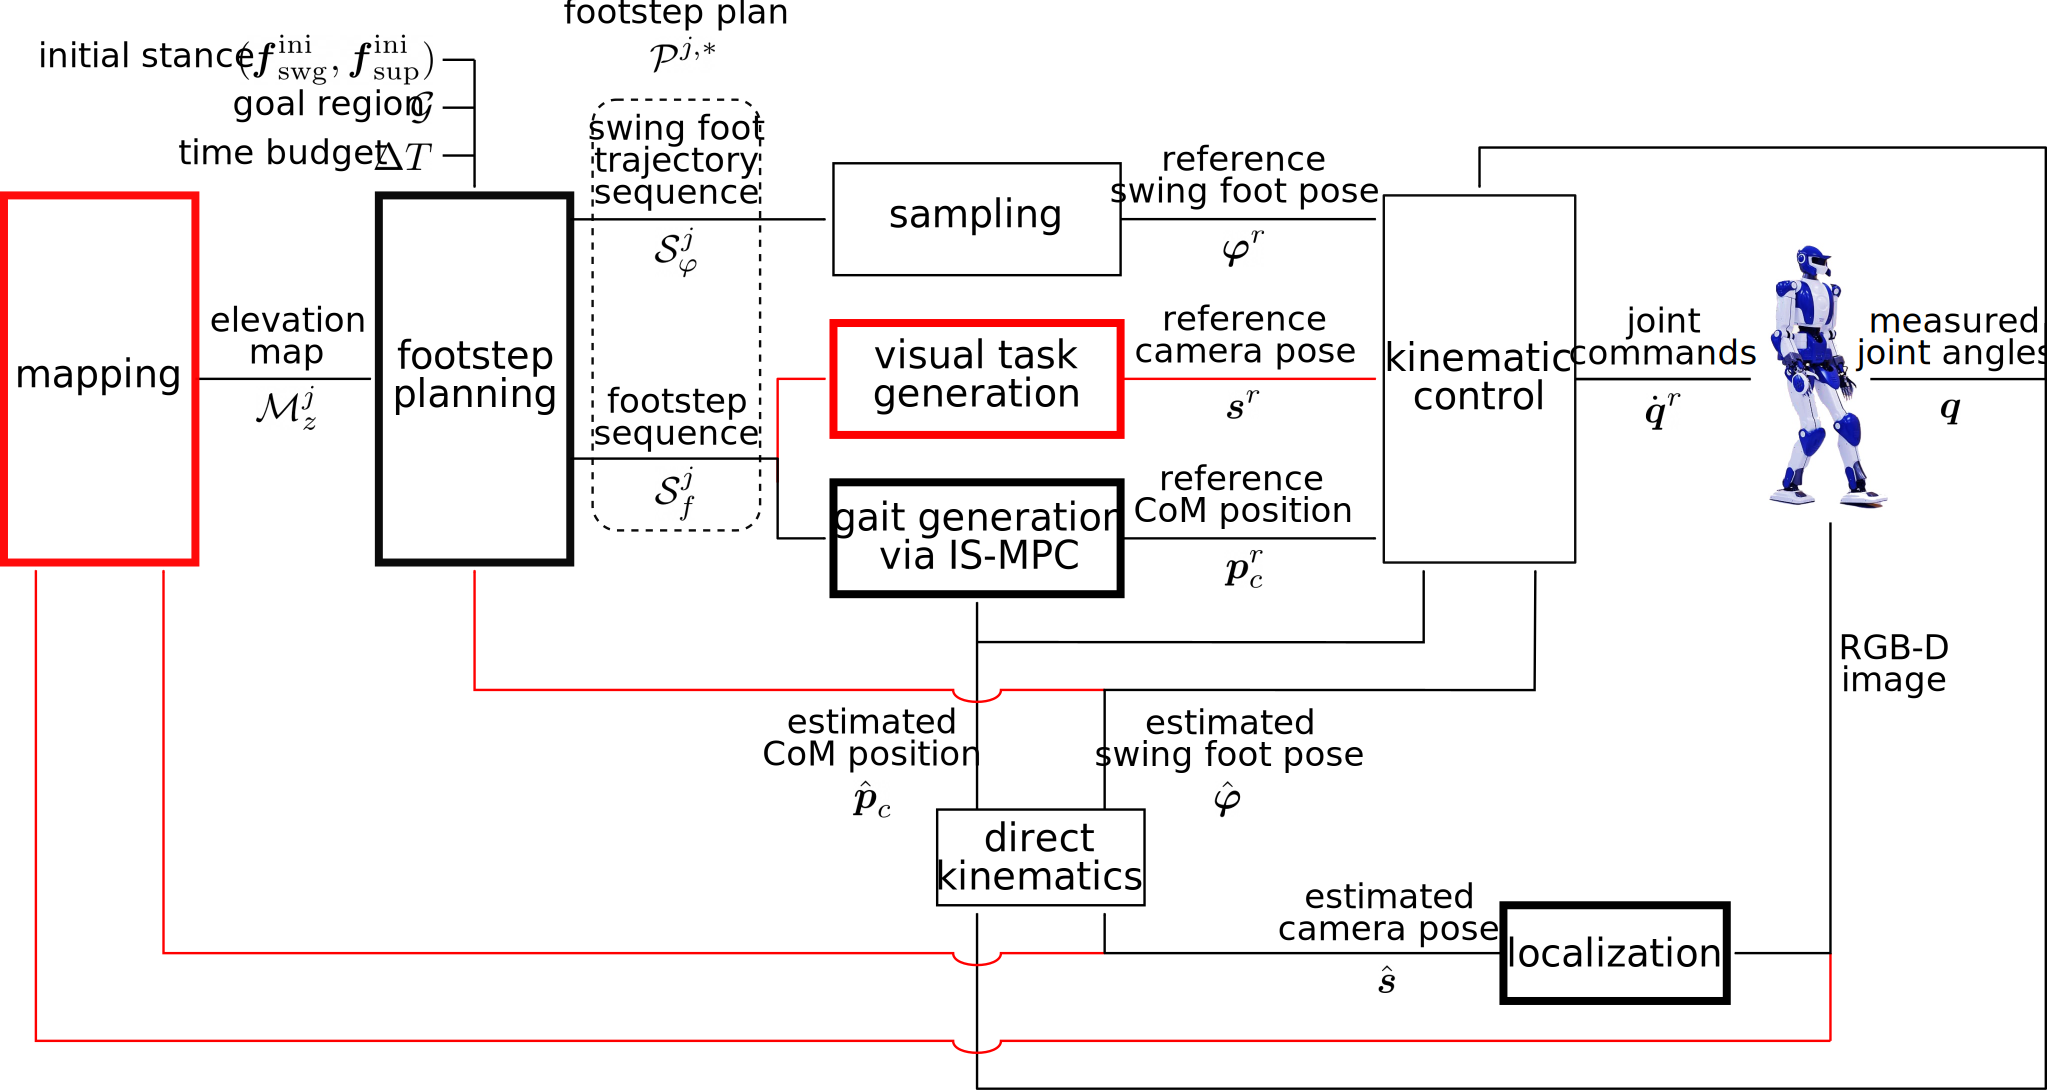
\includegraphics[width=\textwidth]{figures/BlockSchemeOnline.pdf}
\caption{Block scheme of the on-line case. The red blocks and arrows highlight the additional modules and signals compared to the off-line case.}
\label{fig:WoS:blockScheme2}
\end{figure}

The proposed architecture for the on-line case is given in Fig. \ref{fig:WoS:blockScheme2}, where the additional modules and feedback signals are shown in red.

At the beginning, the map ${\cal M}_z$ is initialized combining some limited exogenous knowledge about the starting location of the robot and information available by the head-mounted camera at its initial pose. Such initial map ${\cal M}_z^0$, together with the initial humanoid stance $(\bff_{\rm swg}^{\rm ini}, \bff_{\rm sup}^{\rm ini})$, the goal region $\cal G$ and a preassigned time budget $\Delta T$, is provided to the footstep planner to find a first (possibly partial) footstep plan ${\cal P}^{1,*} = \{ {\cal S}_f^{1}, {\cal S}_\varphi^{1} \}$.

After this initial off-line phase, all the modules run in parallel, generating the humanoid motions in a sensor-based, closed-loop fashion.
%
The mapping module incrementally builds the elevation map ${\cal M}_z$ using the RGB-D images acquired by the humanoid while walking and the estimate $\hat{\bfs}$ of the camera pose produced by the localization module.
To account for changes in ${\cal M}_z$ and take advantage of newly acquired information, the footstep plan is on-line updated and/or extended by repeatedly invoking the footstep planner at every step of the humanoid, with the ultimate objective of reaching $\cal G$. 

More precisely, consider the generic timestamp $t_s^j$, i.e., the beginning of the $j$-th step.
Let $(\hat{\bff}_{\rm swg}^{j}, \hat{\bff}_{\rm sup}^{j})$ be the current stance, with $\hat{\bff}_{\rm swg}^{j}$ and $\hat{\bff}_{\rm sup}^{j}$ the estimates of the swing and support foot poses at $t_s^j$, and ${\cal P}^{j,*} = \{ {\cal S}_f^{j}, {\cal S}_\varphi^{j} \}$ be the current footstep plan -- computed during the previous ($(j-1)$-th) step -- where the sequences of footstep placements and associated swing trajectories are defined as
\begin{gather*}
    {\cal S}_f^j = \{\bff^{j|j}, \dots, \bff^{j+n|j}\}, \\
    {\cal S}_\varphi^j = \{\bfvarphi^{j|j}, \dots, \bfvarphi^{j+n-2|j}\}
\end{gather*}
with their generic elements $\bff^{j+i|j}$ and $\bfvarphi^{j+i|j}$ denoting, respectively, the $(j+i)$-th footstep and trajectory produced by the $j$-th planner invocation, $\bff^{j|j} \approx \hat{\bff}_{\rm swg}^{j}$, $\bff^{j+1|j} \approx \hat{\bff}_{\rm sup}^{j}$ and the last footstep $\bff^{j+n|j}$ henceforth referred to as \textit{subgoal}.
Also, let $(\bff_{\rm swg}^{j+1}, \bff_{\rm sup}^{j+1})$ be the stance that the humanoid is supposed to achieve at $t_s^{j+1} = t_s^j + T_s^j$, with $\bff_{\rm swg}^{j+1} = \hat{\bff}_{\rm sup}^{j}$ and $\bff_{\rm sup}^{j+1} = \bff^{j+2|j}$, after performing the swing trajectory $\bfvarphi^{j|j}$ having duration $T_s^j$.
%
Then, during the time interval $[t_s^j, t_s^{j+1})$, motion execution and footstep planning take place simultaneously as follows.
\begin{itemize}
    \item At any time instant $t \in [t_s^j, t_s^{j+1})$, the current reference position $\bfp_{\rm c}^r$ of the CoM is produced by the gait generator, based on the sequence ${\cal S}_f^j$, similarly to the off-line case; the current reference pose $\bfvarphi^r$ of the swing foot is obtained by sampling the trajectory $\bfvarphi^{j|j}$; moreover, the visual task generator produces the reference pose $\bfs^r$ of the camera frame, given its current estimate $\hat{\bfs}$ and the sequence ${\cal S}_f^j$, that allows to direct the gaze towards the subgoal extracted from ${\cal S}_f^j$, and then to enlarge ${\cal M}_z$ in the area of the current destination. 
    References $\bfp_{\rm c}^r$, $\bfvarphi^r$, $\bfs^r$, together with their estimates $\hat{\bfp}_{\rm c}$, $\hat{\bfvarphi}$, $\hat{\bfs}$, are passed to the kinematic controller to compute the joint commands $\dot{\bfq}^r$ for the robot.
    \item At $t_s^j$, the footstep planner is invoked providing in input the stance $(\bff_{\rm swg}^{j+1}, \bff_{\rm sup}^{j+1})$, the goal region $\cal G$, a time budget equal to $T_s^j$, and the elevation map ${\cal M}_z^j$ currently available by the mapping module.
    At $t_s^{j+1}$, the planner returns a new footstep plan ${\cal P}^{j+1,*} = \{ {\cal S}_f^{j+1}, {\cal S}_\varphi^{j+1}\}$, where the sequences ${\cal S}_f^{j+1}$ and ${\cal S}_\varphi^{j+1}$ are defined similarly to ${\cal S}_f^{j}$ and ${\cal S}_\varphi^{j}$, $\bff^{j+1|j+1} = \bff_{\rm swg}^{j+1}$ and $\bff^{j+2|j+1} = \bff_{\rm sup}^{j+1}$. 
    The first element $\bfvarphi^{j+1|j+1}$ of ${\cal S}_\varphi^{j+1}$ will define the next ($(j+1)$-th) step of the humanoid. 
\end{itemize}

Note that, while the footstep planner will make use of a fixed map $\mathcal{M}_z^j$ during the time interval $[t_s^j, t_s^{j+1})$, the map $\mathcal{M}_z$ will continuously be updated by the mapping module during the same time interval, which will generally provide a different map $\mathcal{M}_z^{j+1}$ for the next invocation of the planner.

Clearly, in the on-line case, only the quality of the partial footstep plans can be accounted for, ultimately leading to an overall plan that is globally suboptimal. 

\subsection{Mapping}
\label{sec:WoS:onlineCase:MappingModule}

At the generic time instant, the mapping module receives in input the last RGB-D image acquired by the head-mounted camera and the current estimate $\hat{\bfs}$ of the camera pose produced by the localization module. 
It is responsible for integrating such newly acquired information into the elevation map
$\mathcal{M}_z$.

First, the depth data extracted from the RGB-D image are used to construct a point cloud.
Then, the latter is given in input, together with the estimate $\hat{\bfs}$ and a sensor noise model, to Elevation Mapping \cite{FaBlHu:18}, an open source framework designed for rough terrain mapping; this accordingly updates a local (limited around the robot)
representation of the environment in the form of a 2.5D grid map (see Assumption A1).
Finally, such local map is integrated into $\mathcal{M}_z$ in order to maintain a global representation of the explored area of the environment.

The mapping module, at the time $t_s^j$ of the generic $j$-th invocation of the footstep planner, provides it with a copy $\mathcal{M}_z^j$ of the available map $\mathcal{M}_z$.
Meanwhile, during the planner operation, the map $\mathcal{M}_z$ is continuously updated through the process described above.

\subsection{Sensor-based footstep planning}
\label{sec:WoS:onlineCase:FootstepPlanner}

This module consists in a sensor-based version of the footstep planner proposed in Sect. \ref{sec:WoS:offlineCase:FootstepPlanner} which works using the knowledge about the environment incrementally acquired by the robot during motion. 

The input data for the $j$-th invocation of the footstep planner are the next robot stance $(\bff_{\rm swg}^{j+1}, \bff_{\rm sup}^{j+1})$, the goal region $\cal G$, the time budget ${\Delta T}^j$ and the elevation map ${\cal M}_z^j$. 
Given an optimality criterion, the footstep planner returns the best footstep plan ${\cal P}^{j+1,*}$, found within ${\Delta T}^j$, either leading to $\cal G$ or terminating in proximity of the frontier of ${\cal M}_z^j$.
The latter case is typical whenever $\cal G$ is not included in ${\cal M}_z^j$, e.g., due to occlusions or simply being placed far from the robot.

The planning algorithm builds a tree $\mathcal{T}^{j+1}$ reusing portions of the tree $\mathcal{T}^{j}$ built up to the previous invocation. 
In this tree, vertexes and edges are defined as described in Sect. \ref{sec:WoS:offlineCase:FootstepPlanner}, with the only difference that a vertex $v = (\bff_{\rm swg}, \bff_{\rm sup})$ can contain a support footstep $\bff_{\rm sup}$ whose $z$-coordinate is unspecified, indicating that ${\cal M}_z^j$ does not provide enough information (in a sense formally defined in the following) about the ground under the foot at $\bff_{\rm sup}$. 
Vertexes with this characteristic represent stances located on the frontier of ${\cal M}_z^j$ and thus indicate possible direction for further exploration of the environment. 
%
The generic invocation consists of: initializing, updating and expanding the tree. These individual steps are described in the following.

{\bf Initializing}: The vertex $v^{\rm root} = (\bff_{\rm swg}^{\rm root}, \bff_{\rm sup}^{\rm root})$ of $\mathcal{T}^{j}$ that is closest to $(\bff_{\rm swg}^{j+1}, \bff_{\rm sup}^{j+1})$ is identified. To this end, we define a stance-to-stance metric as
\begin{equation}
    \label{eq:WoS:metricIdentifyRoot}
    \zeta(v, v') = \gamma(\bff_{\rm swg}, \bff'_{\rm swg}) + \gamma(\bff_{\rm sup}, \bff'_{\rm sup}) 
\end{equation}
where $\gamma(\cdot)$ is the footstep-to-footstep metric defined in (\ref{eq:WoS:footstepToFootstepMetric}).
The subtree of $\mathcal{T}^{j}$ rooted at $v^{\rm root}$ is extracted (including $v^{\rm root}$ itself) and represents the initial version of $\mathcal{T}^{j+1}$.
To match the stance that the humanoid is supposed to reach at the end of the simultaneously executed step, $v^{\rm root}$ is modified by relocating $\bff_{\rm swg}^{\rm root}$ to $\bff_{\rm swg}^{j+1}$ and $\bff_{\rm sup}^{\rm root}$ to $\bff_{\rm sup}^{j+1}$. \hfill $\blacktriangleleft$

{\bf Updating}: At this point, requirements R1--R3 are satisfied by construction in $\mathcal{T}^{j+1}$ according to the previous map $\mathcal{M}_z^{j-1}$.
Then, R1--R3 must now be checked in $\mathcal{T}^{j+1}$ using the most recent map $\mathcal{M}_z^{j}$, consequently updating vertexes and edges in order to satisfy them.
To this end, we perform a pre-order traversal of $\mathcal{T}^{j+1}$ as described in the following.

When a vertex $v = (\bff_{\rm swg}, \bff_{\rm sup})$ is visited, it is  modified\footnote{This modification is not made on $v^{\rm root}$ as it corresponds to the stance that the robot must reach at the end of the simultaneously executed step.} by relocating its swing footstep to the support footstep $\bff_{\rm sup}^{\rm parent}$ of its parent $v^{\rm parent} = (\bff_{\rm swg}^{\rm parent}, \bff_{\rm sup}^{\rm parent})$, and setting the $z$ coordinate $z_{f, \rm sup}$ of $\bff_{\rm sup}$ according to $\mathcal{M}_z^{j}$.
%the current knowledge about the height of the ground contained in the cells of ${\cal M}_z^j$ belonging to, or overlapping with, the footprint at $\bff_{\rm sup}$.
In particular, consider the cells of ${\cal M}_z^j$ belonging to, or overlapping with, the footprint at $\bff_{\rm sup}$; let $n_{\rm k}$ and $n_{\rm u}$ be the number of these cells whose height is known and unknown, respectively. If the rate of cells with known height is larger than a predefined threshold $\bar{n}$, i.e.,
\begin{equation*}
    \frac{n_{\rm k}}{n_{\rm k} + n_{\rm u}} > \bar{n},    
\end{equation*}
$z_{f, \rm sup}$ is set to the average value of the $n_{\rm k}$ known heights. 
Otherwise, $z_{f, \rm sup}$ is left unspecified.

Once $v$ has been updated, requirements R1--R3 are checked similarly to what was done in the off-line case, with the only two differences described in the following.
%accounting for possible noise and/or incomplete information in $\mathcal{M}_z^{j}$.
\begin{itemize}
    \item If $z_{f, \rm sup}$ is unspecified, requirements R1--R3 are checked conjecturing that it is equal to the $z$-component $z_{f, \rm swg}$ of $\bff_{\rm swg}$.
    %
    \item Requirement R1 is considered satisfied if for each of the $n_{\rm k}$ known heights, the net variation from $z_{f, \rm sup}$ does not exceed a predefined threshold $\bar{z}$, i.e.,
    \begin{equation*}
        |z_{\rm k} - z_{f, \rm sup}| \leq \bar{z}.
    \end{equation*}
    with $z_{\rm k}$ the generic known height among the $n_{\rm k}$ available.
    %\item Requirement R1 is considered satisfied if for each cell of ${\cal M}_{z}^j$ belonging to, or overlapping with, the footprint at $\bff_{\rm sup}$, the absolute difference between the contained height $z$ and $z_{f, \rm sup}$ does not exceed a predefined threshold $\bar{z}$, i.e.,
    %\begin{equation*}
    %    |z - z_{f, \rm sup}| \leq \bar{z}.
    %\end{equation*}
\end{itemize}

If any requirement among R1--R3 is violated, vertex $v$ is removed from $\mathcal{T}^{j+1}$, along with its descendants.
Otherwise, the edge connecting $v$ to $v^{\rm parent}$ is replaced by the trajectory $\bfvarphi^{\rm parent}$ generated while checking R3; the set ${\cal V}_{\rm child}$ of child vertexes of $v$ is retrieved, and the procedure is recursively invoked on them. 
To guarantee on-line performance and save time to be used for expanding $\mathcal{T}^{j+1}$, recursion is stopped on vertexes having a maximum depth $\bar{\kappa}$. \hfill $\blacktriangleleft$

{\bf Expanding}: Once $\mathcal{T}^{j+1}$ has been updated, it can be further expanded in the map $\mathcal{M}_z^j$.
Let ${\Delta T}_{\rm e}$ be the time elapsed since the beginning of the current invocation of the footstep planner, i.e., the time spent in initializing and updating $\mathcal{T}^{j+1}$.
The expansion of $\mathcal{T}^{j+1}$ works iteratively as described in Sect. \ref{sec:WoS:offlineCase:FP:PlannerOverview} using the remaining portion of the time budget ${\Delta T}^j - {\Delta T}_{\rm e}$ and the map $\mathcal{M}_z^j$, with the following modifications.
\begin{itemize}
    \item The choice of the $z$-coordinate for a candidate footstep $\bff_{\rm sup}^{\rm cand}$ and the check of requirements R1--R3 are done exactly as when updating a generic vertex. 
    \item A vertex whose support footstep has unspecified $z$-coordinate cannot be set as parent of another vertex.
    Then, such vertexes are excluded both when selecting the vertex $v^{\rm near}$ for an expansion attempt and when choosing a parent for a candidate vertex $v^{\rm cand}$. \hfill $\blacktriangleleft$
\end{itemize} 

Similarly to the off-line case, when the assigned time budget ${\Delta T}^j$ runs out, tree expansion is stopped and the set ${\cal V}_{\rm goal}$ of vertexes $v$ such that $\bfp_{f,{\rm sup}} \in {\cal G}$ is retrieved.
%
If ${\cal V}_{\rm goal}$ is not empty, the vertex $v^*$ with minimum cost is selected as in (\ref{eq:WoS:BestVertex}).
%
Otherwise, if ${\cal V}_{\rm goal}$ is empty, the planner retrieves the set ${\cal V}_{\rm fron}$ containing all vertexes of $\mathcal{T}^{j+1}$ having at least one child vertex whose support footstep has unspecified $z$-coordinate.
In practice, vertexes in ${\cal V}_{\rm fron}$ contain stances located in proximity of the frontier of the current map $\mathcal{M}_z^j$.
Then, the vertex $v^*$ is selected as
\begin{equation}
    \label{eq:WoS:BestVertexSubgoal}
    v^* = \underset{v \in {\cal V}_{\rm fron}}{\arg\!\min} \ c(v)+g(v)
\end{equation}
where $g(v)$ represents the \textit{cost-to-go} of vertex $v$, i.e., a lower-bound on the minimum cost to reach $\mathcal{G}$ from $v$.
A possible choice for $g(v)$ when minimizing the number of steps along the plan will be described in Sect. \ref{sec:WoS:onlineCase:Simulations}.

Finally, the footstep plan ${\cal P}^{j+1,*}$ is retrieved from the branch of $\mathcal{T}^{j+1}$ joining the root to $v^*$. 
Clearly, if ${\cal V}_{\rm goal}$ is not empty, ${\cal P}^{j+1,*}$ will be a complete footstep plan leading to $\mathcal{G}$; otherwise, ${\cal P}^{j+1,*}$ will be a partial footstep plan leading in the direction of an unknown area of the environment whose exploration is considered useful -- according to the adopted cost-to-go -- to proceed towards $\mathcal{G}$. 

\subsection{Visual task generation}
\label{sec:WoS:onlineCase:VisualTaskGeneration}

At any time instant during the execution of the generic $j$-th step, given the current estimate $\hat{\bfs}$ of the camera pose and the subgoal $\bff^{j+n|j}$, which is readily extracted from the current sequence $\mathcal{S}_f^j$ of footstep placements, the visual task generator is in charge of producing a suitable reference $\bfs^r$ of the camera pose which aims at directing the gaze towards the current destination of the robot. 
The rationale beyond this choice is that, since the current footstep plan terminates in an area on the frontier of the map $\mathcal{M}_z$ that is considered promising for goal-oriented exploration of the environment, looking in the direction of $\bff^{j+n|j}$ allows to enlarge the map in that particular area. In principle, whenever possible, this will privilege further extension of the footstep plan in that promising direction.

To compute $\bfs^r$, one possibility consists in adopting an image-based visual servoing scheme \cite{ChHuCo:16}. 
In particular, one may define a virtual feature in the image plane of the camera at $\hat{\bfs}$ associated to the representative point $\bfp_f^{j+n|j}$ of the subgoal footstep $\bff^{j+n|j}$.
Then, the reference pose $\bfs^r$ of the camera frame can be computed so as to keep such feature at the center of the image plane.

The produced reference pose $\bfs^r$ is passed to the kinematic controller which, in practice, only controls the camera yaw and pitch angles.


\subsection{Simulations}
\label{sec:WoS:onlineCase:Simulations}

\begin{figure}
    \centering
    \includegraphics[width=\textwidth]{figures/OnlineCorridor.png}
    \caption{The on-line footstep planner in the scenario \textit{Corridor} minimizing the number of steps. Here the planner finds a footstep sequence of 54 steps.}
    \label{fig:WoS:onlineCase:Corridor:Simulation}
\end{figure}
\begin{figure}
    \centering
    \includegraphics[width=\textwidth]{figures/OnlineMazeDynamic.png}
    \caption{The on-line footstep planner in the environment \textit{Maze} minimizing the number of steps. The environment is dynamic, namely the elevation map can be changed by moving obstacles around. Here the planner finds a footstep sequence of 106 steps.}
    \label{fig:WoS:onlineCase:MazeDynamic:Simulation}
\end{figure}
\begin{figure}
    \centering
    \includegraphics[width=\textwidth]{figures/OnlineMazeStopandgo.png}
    \caption{The on-line footstep planner in the dynamic environment \textit{Maze} minimizing the number of steps. Here the planner finds a footstep sequence of 103 steps.}
    \label{fig:WoS:onlineCase:MazeStopAndGo:Simulation}
\end{figure}

In this section we present simulations obtained with the discussed architecture for the on-line case. Parameters are set to the same values of Sects. \ref{sec:WoS:offlineCase:FP:PlanningResults} and \ref{sec:WoS:offlineCase:Simulations}, with the only exception of setting $k_\gamma = 1$ in \eqref{eq:WoS:footstepToFootstepMetric} when used in \eqref{eq:WoS:metricIdentifyRoot}, $\bar{n}=0.9$, $\bar{z}=0.02$ and ${\bar{\kappa}}=5$. For each $j$-th invocation of the footstep planner the time budget $\Delta T^j$ is set to $T_{ss}+T_{ds}$. In all performed simulations, the quality criteria considered by the footstep planner is the number of steps, while the \textit{cost-to-go} of each vertex $v$ is an underestimation of the number of steps needed to reach the goal region $\mathcal{G}$ from the double support configuration specified by $v$. This value is computed as the distance between the position of the support foot specified by $v$ and $\mathcal{G}$, divided by the longest step among the catalogue of primitives $U$. 
%In all our simulations the planner is replanning the footsteps every second (which corresponds to the duration of a step of the robot).

Figure \ref{fig:WoS:onlineCase:Corridor:Simulation} shows the robot walking in the scenario \textit{Corridor} together with the reconstructed elevation map. Here, the planner continuously receives an updated version of the map, which is built while the robot moves. Initially (first snapshot) the robot starts exploring its surrounding environment, moving towards the end of the corridor (second snapshot). As soon as the footstep planner realizes that the room is closed, it replans a sequence of footsteps which brings the robot outside the corridor (third snapshot). The robot keeps exploring the environment, going up and down the stairs and avoiding the obstacles placed along the path (fourth and fifth snapshot). Finally, the robot reaches the desired goal region (sixth snapshot).

Figure \ref{fig:WoS:onlineCase:MazeDynamic:Simulation} shows the robot accomplishing the locomotion task in the scenario \textit{Maze}. In this case the scenario was rendered dynamic by manually moving the obstacles at runtime. Here, the planner is facing the additional challenge of operating under continuous changes in the elevation map, which reflects the new locations of the obstacles. The robot starts by moving outside the initial room (first snapshot), choosing the path on its right (second snapshot). The footstep plan is invalidated by placing obstacles in front of the robot, forcing the robot to choose the other direction (third snapshot). The footstep planner correctly drives the robot towards the other area of the maze (fourth snapshot), making it go up and down the staircase (fifth snapshot), avoiding another obstacle which is placed in front of the robot right before reaching the goal region (sixth snapshot).

Figure \ref{fig:WoS:onlineCase:MazeStopAndGo:Simulation} shows a situation, again in a dynamic version of the scenario \textit{Maze}, in which the planner reaches a point in which is not able to find a new subgoal. This occurs when, once the time budget expires, both $\mathcal{V}_{\rm goal}$ and $\mathcal{V}_{\rm fron}$ are empty.
For example, this may happen when the humanoid must exit a long corridor or when dynamic obstacles invalidate large portion of the created tree.
In this specific situation, a simple solution consists in keeping the portion of the current footstep plan that is still valid after the updating step of the planner. 
If this happens multiple times in a row, the robot reaches the subgoal and stops. At this point, the footstep planner is invoked with an unlimited time budget and terminates as soon as a new subgoal is found. As before, the robot starts by moving outside the initial room, moving towards its left (first and second snapshots). The footstep plan is invalidated by moving an obstacle in front of the robot (third snapshots), which stops its motion upon reaching the current subgoal (fourth snapshot). As soon as the footstep planner finds a new subgoal, the robot starts moving again (fifth snapshot), eventually reaching the desired goal region (sixth snapshot).

Clips of the described simulations are included in the accompanying video.% available at the same link indicated in Sect. \ref{sec:WoS:offlineCase:Simulations}.


\section{Discussion}
\label{sec:WoS:discussion}

The proposed approach integrates several components and is designed to work both off-line and on-line. 
Since, to the best of our knowledge, no existing method can address the same wide range of situations, we focus in the following on the two main components (footstep planning and gait generation) separately.


As a representative of the state of the art in footstep planning, we selected the algorithm in~\cite{Griffin_ICRA2019}, which uses a weighted $A^\ast$ algorithm to search for optimal footstep sequences on uneven ground\footnote{The algorithm in~\cite{Griffin_ICRA2019} actually contemplates the possibility of tilted surfaces, but obviously works in a world of stairs as a particular case.}. At each iteration, the vertex providing the lowest estimate for the path cost is expanded. This estimate is computed by adding to the cost of the vertex a heuristic cost-to-go, given by the distance to the goal divided by the maximum step length and multiplied by a weight $w\ge 1$, which can be used to increase the bias towards the goal region. The main difference with respect to our approach lies in the expansion mechanism, which is deterministic in~\cite{Griffin_ICRA2019} and probabilistic in our method. 


Both our scheme and the weighted $A^\ast$ approach use a catalogue of primitives. In order to perform a fair comparison, we use for the weighted $A^\ast$ approach the same catalogue described in Sect.~\ref{sec:WoS:offlineCase:FP:PlanningResults}. As for the optimality criterion, we aim to minimize the number of footsteps, corresponding to an edge cost given by (\ref{eq:WoS:costSteps}). In order to allow for the possibility that our implementation might not be the most efficient, we assigned to the weighted $A^\ast$ planner a time budget of $100$~s, which is four times the largest budget used when testing our planner. 

The results obtained showed that standard $A^\ast$ search, corresponding to $w=1$, is unable to find solutions within the allotted time budget in any of the considered scenarios. 
By increasing $w$, weighted $A^\ast$ performs rather well in scenarios where the solution does not involve considerable backtracking ({\em Rod} and {\em Spacious}), but fails to find the solution in any other scenario. In particular, Table~\ref{tab:benchmark-wastar-w5} collects the results obtained for $w=5$. 
These results should be compared to those in Table~\ref{tab:benchmark:off-line:steps}, which show that our approach has a $100$\% success rate with a fourth of the time budget. 
We also ran tests with larger weights ($w=10$, $w=25$), obtaining results that are essentially identical, with slightly longer paths and no increase in the success rate. 

Indeed, the outcome of the above comparison was rather predictable.
It is well known that weighted $A^\ast$ works quite well in environments where the path leading to the goal does not deviate significantly from a straight line. However, as acknowledged by the authors of~\cite{Griffin_ICRA2019}, its performance may degrade severely in the scenarios that require even mild amounts of backtracking. 

\begin{table}
    \centering
    \begin{tabular}{*{5}{c}}
        %Scenario & $\Delta T$ [s] & Cost & Iters & Tree Size \\
        %\hline
        %\textit{Rod} & 1.45 & 22.0 & 650 & 4049 \\
        %\textit{Ditch} & 100.0 & Fail & 11687 & 21911 \\
        %\textit{Corridor} & 100.0 & Fail & 12343 & 22483 \\
        %\textit{Spacious} & 0.085 & 31.0 & 34 & 546 \\
        %\textit{Maze} & 100.0 & Fail & 9546 & 22333
        Scenario & Cost & Iters & Tree Size \\
        \hline
        \textit{Rod} & 22.0 & 650 & 4049 \\
        \textit{Ditch} & Fail & 11687 & 21911 \\
        \textit{Corridor} & Fail & 12343 & 22483 \\
        \textit{Spacious} & 31.0 & 34 & 546 \\
        \textit{Maze} & Fail & 9546 & 22333
    \end{tabular}
    \caption{Performance of the off-line weighted $A^\ast$ footstep planner when minimizing the number of steps ($w=5.0$).}
    \label{tab:benchmark-wastar-w5}
\end{table}

As for the gait generation component, there are several alternatives to our method that employ MPC on reduced-order models. The advantage of the proposed approach lies in the introduction of the stability constraint, which allows to prove rigorously recursive feasibility and internal stability of the MPC scheme. The effectiveness of this approach was extensively analyzed in \cite{ScDeLaOr:20}, by means of comparisons to state-of-the-art schemes. What we proposed in this paper is an extension accounting for the fact that the CoM height changes. Based on the additional theoretical results which we proved (namely, Props.~\ref{prop:velocityBound} and~\ref{prop:conservative-box}), we can claim that our 3D gait generation retains the same properties of the original 2D scheme. 

\section{Conclusions} 
\label{sec:WoS:Conclusions}


In this paper, we addressed the problem of motion generation for a humanoid robot that must reach a certain goal region walking in an environment consisting of horizontal patches located at different heights, called \textit{world of stairs}.
We considered two versions of such problem: the off-line and on-line case. 
In the first, the geometry of the environment is completely known in advance, while in the second, it is reconstructed by the robot itself during motion using an on-board sensor. In both cases, available information about the environment is maintained in the form of an elevation map. 

For the off-line case, we proposed an architecture working in two main stages: footstep planning and gait generation.
First, a feasible footstep plan leading to the goal region is off-line computed using a randomized algorithm that takes into account the plan quality specified by a given optimality criterion.
Then, an intrinsically stable MPC-based scheme computes a CoM trajectory that realizes the found footstep sequence, while guaranteeing dynamic balance and boundedness of the CoM w.r.t. the ZMP at all time instants.

For the on-line case, we proposed an extension of the architecture for the off-line case where footstep plans are computed in parallel to gait generation and map building.
To this end, we presented a sensor-based version of the footstep planner that uses the knowledge about the environment incrementally acquired by the robot during motion.

We validated  the proposed architectures by providing simulation results obtained in CoppeliaSim on the HRP-4 humanoid robot in scenarios of different complexity.

Our future work will explore several directions, such as
\begin{enumerate}
    \item providing a formal proof of asymptotic optimality of the proposed footstep planner;
    \item developing a more general version of the proposed approach to deal with arbitrary terrains, removing the world of stairs assumption;
    \item implementing the presented architectures on a real humanoid robot;
    \item extending them to the case of large-scale and multi-floor environments.
\end{enumerate}

\subsection{Pseudocode}
\label{sec:WoS:Pseudocode}
  
We report here a pseudocode description of the footstep planners presented in Sections \ref{sec:WoS:offlineCase:FootstepPlanner} and \ref{sec:WoS:onlineCase:FootstepPlanner}, along with the relevant procedures. 

\begin{algorithm}%[!t]
	\small
	\removelatexerror
	\label{alg:FootstepPlanner}
    %\caption{FootstepPlanner$(({\bff}_{\rm swg}^{\rm ini}, {\bff}_{\rm sup}^{\rm ini}), {\cal G}, {\Delta T}, {\cal M}_z)$}
	
	\caption{FootstepPlanner}
	\KwIn{$({\bff}_{\rm swg}^{\rm ini}, {\bff}_{\rm sup}^{\rm ini}), {\cal G}, {\Delta T}, {\cal M}_z$}
	\vspace{2pt}
	\KwOut{${\cal P}^*$}
    \BlankLine
    
	$v^{\rm ini}$ $\leftarrow$ $({\bff}_{\rm swg}^{\rm ini}$, ${\bff}_{\rm sup}^{\rm ini})$\; 
	
	AddVertex$(\cal T$, $\emptyset$, $v^{\rm ini}$, $\emptyset)$\;
	
	ExpandTree$(\cal T$, ${\Delta T}$, ${\cal M}_z)$\;
	
    ${\cal P}^*$ $\leftarrow$ RetrieveBestPlan$({\cal T}, {\cal G})$\;	
    \Return{${\cal P}^*$}\;
\end{algorithm}

\begin{procedure}%[!t]
	\small
	\removelatexerror
	\label{proc:ExpandTree}
	%\caption{ExpandTree(${\cal T}$, ${\Delta T}$, ${\cal M}_z$)}
	
	\caption{ExpandTree()}
	\KwIn{${\cal T}, {\Delta T}, {\cal M}_z$}
	\vspace{2pt}
	\KwOut{none}
    \BlankLine
    
	\While{\rm \textbf{not} TimeExpired$({\Delta T})$}{
	 	$\bfp_{xy}^{\rm rand}$ $\leftarrow$ SamplePoint$()$\;
	 	$v^{\rm near}$ $\leftarrow$ NearestVertex$(\mathcal{T}, \bfp_{xy}^{\rm rand})$\;
	 	$\bff^{\rm cand}_{\rm sup}$ $\leftarrow$ GenerateCandidateFootstep$(\bff_{\rm sup}^{\rm near}, U, \mathcal{M}_z)$\;
	 	
	 	\If{\rm R1$(\bff^{\rm cand}_{\rm sup})$ \rm \textbf{and} \rm R2$(\bff^{\rm cand}_{\rm sup}, \bff^{\rm near}_{\rm sup})$}{
	 	 	$\bfvarphi^{\rm near}$ $\leftarrow$ SwingTrajectoryEngine$(\bff_{\rm swg}^{\rm near}, \bff_{\rm sup}^{\rm cand})$\;
		 	
		 	\If{\rm R3$(\bfvarphi^{\rm near}, (\bff^{\rm near}_{\rm sup}, \bff^{\rm cand}_{\rm sup}))$}{
		 	    $v^{\rm cand}$ $\leftarrow (\bff^{\rm near}_{\rm sup}, \bff^{\rm cand}_{\rm sup})$\;
		 		
		 		$\mathcal{N} \leftarrow$ Neighbors$(\mathcal{T}, v^{\rm cand})$\;
		 		
		 		$(v^{\rm min}, \bfvarphi^{\rm min}) \leftarrow$ ChooseParent$(\mathcal{T}, \mathcal{N}, v^{\rm near}, v^{\rm cand}, \bfvarphi^{\rm near})$\;
		 		
                $v^{\rm new} \leftarrow (\bff^{\rm min}_{\rm sup}, \bff^{\rm cand}_{\rm sup})$\;
		 		
		 		AddVertex$(\mathcal{T}, v^{\rm min}, v^{\rm new}, \bfvarphi^{\rm min})$\;	
		 		
		 		ReWire$(\mathcal{T}, \mathcal{N}, v^{\rm new})$\;	
		 	}   			
	 	}    
	 }
	 \Return{}\;
\end{procedure}

\begin{procedure}%[!t]
	\small
	\removelatexerror
	\label{proc:genswgtraj}
	
	%\caption{SwingTrajectoryEngine($\bff^a$, $\bff^b$)}
	\caption{SwingTrajectoryEngine()}
	\KwIn{$\bff^a$, $\bff^b$}
	\KwOut{$\bfvarphi^a$}
    \BlankLine

	$h$ $\leftarrow$ $h^{\rm min}$\;
	
	\While{$h \leq h^{\rm max}$}{
		$\bfvarphi^a \leftarrow$ DeformTrajectory$(\bff^a, \bff^b, h)$\;		 	
	
	   	\If{\rm CollisionFree$(\bfvarphi^a)$}{
            \Return{$\bfvarphi^a$}\;	   	
	   	}
		
	    $h \leftarrow h + \Delta h$\;
	}
			
	\Return{$\emptyset$}\;	
\end{procedure}

\begin{procedure}%[!t]
	\small
	\removelatexerror
	\label{proc:chooseparent}
	%\caption{ChooseParent($\cal T$, $\cal N$, $v^{\rm near}$, $v^{\rm cand}$, $\bfvarphi^{\rm cand}$)}
	
	\caption{ChooseParent()}
	\KwIn{${\cal T}, {\cal N}, v^{\rm near}, v^{\rm cand}, \bfvarphi^{\rm cand}$}
	\vspace{2pt}
	\KwOut{$v^{\rm min}, \bfvarphi^{\rm min}$}
    \BlankLine
	
	$v^{\rm min}$ $\leftarrow$ $v^{\rm near}$\;
	$\bfvarphi^{\rm min}$ $\leftarrow$ $\bfvarphi^{\rm cand}$\;
	$c^{\rm min}$ $\leftarrow$ $c(v^{\rm near}) + l(v^{\rm near}, v^{\rm cand})$\;
	
	\ForEach{$v'$ $\in$ $\cal N$}{
    	\If{\rm R2$(\bff_{\rm sup}^{\rm cand}, \bff'_{\rm sup})$}{
    		$\bfvarphi' \leftarrow$ SwingTrajectoryEngine$(\bff'_{\rm swg}, \bff_{\rm sup}^{\rm cand})$\;
    		
    		\If{\rm R3$(\bfvarphi', (\bff'_{\rm sup}, \bff_{\rm sup}^{\rm cand}))$ \rm \textbf{and} $c(v') +l(v', v^{\rm cand}) < c^{\rm min}$}{
				$v^{\rm min}$ $\leftarrow$ $v'$\;
				$\bfvarphi^{\rm min}$ $\leftarrow$ $\bfvarphi'$\;
				$c^{\rm min}$ $\leftarrow$ $c(v') +l(v', v^{\rm cand})$\;
    		}
    	}
	}
	\Return{$(v^{\rm min}$, $\bfvarphi^{\rm min})$}\;	
\end{procedure}

\begin{procedure}%[!t]
	\small
	\removelatexerror
	%\caption{ReWire($\cal T$, $\cal N$, $v^{\rm new}$)}
	\label{proc:rewire}
    \caption{ReWire()}
	\KwIn{${\cal T}, {\cal N}, v^{\rm new}$}
	\vspace{2pt}
	\KwOut{none}
    \BlankLine
			
	\ForEach{$v'$ $\in$ $\cal N$}{
        \If{\rm R2$(\bff'_{\rm sup}, \bff^{\rm new}_{\rm sup})$}{
 	 	
 	 	    $\bfvarphi^{\rm new} \leftarrow$ SwingTrajectoryEngine$(\bff_{\rm swg}^{\rm new}, \bff'_{\rm sup})$\;
	 	
    	 	\If{\rm $R3(\bfvarphi^{\rm new}, (\bff'_{\rm swg}, \bff'_{\rm sup}))$ \textbf{and} $c(v^{\rm new}) + l(v^{\rm new}, v') < c(v')$}{
                
                UpdateVertex$({\cal T}, v', (\bff_{\rm sup}^{\rm new}, \bff'_{\rm sup}))$\;
                
                UpdateEdge$({\cal T}, v^{\rm new}, v', \bfvarphi^{\rm new})$\;
                
                ${\cal V}_{\rm child} \leftarrow$ ChildVertexes$({\cal T}, v')$\;
                
                \ForEach{$v''$ $\in$ ${\cal V}_{\rm child}$}{
                    $\bfvarphi'$ $\leftarrow$ SwingTrajectoryEngine$(\bff'_{\rm swg}, \bff''_{\rm sup})$\;
                    
                    \eIf{$\bfvarphi' \neq \emptyset$}{
                        UpdateEdge$({\cal T}, v', v'', \bfvarphi')$\;
                    }
                    {
                        RemoveSubtree$({\cal T}, v'')$\; 	
                    }
    	 	    }
                 	   
    	 	}
 	    }
	}
		
	\Return\;	

\end{procedure}

\begin{algorithm}%[!t]
	\small
	\removelatexerror
	\label{alg:AnytimeFootstepPlanner}
    %\caption{SensorBasedFootstepPlanner$(({\bff}_{\rm swg}^{j+1}, {\bff}_{\rm sup}^{j+1}), {\cal G}, {\Delta T}^j, {\cal M}_z^j)$}
	
	\caption{SensorBasedFootstepPlanner}
	\KwIn{$({\bff}_{\rm swg}^{j+1}, {\bff}_{\rm sup}^{j+1}), {\cal G}, {\Delta T}^j, {\cal M}_z^j$}
	\vspace{2pt}
	\KwOut{${\cal P}^{j+1,*}$}
    \BlankLine

    $({\cal T}^{j+1}, v^{\rm root})$ $\leftarrow$ InitializeTree$({\cal T}^j, ({\bff}_{\rm swg}^{j+1}, {\bff}_{\rm sup}^{j+1}))$\; 
	
    ${\cal V}_{\rm child}$ $\leftarrow$ ChildVertexes$({\cal T}^{j+1}, v^{\rm root})$\;
	\ForEach{$v'$ $\in$ ${\cal V}_{\rm child}$}{
        UpdateTree$({\cal T}^{j+1}, v', {\cal M}_z^j)$\;
    } 	

	ExpandTree$({\cal T}^{j+1}, {\Delta T}^j - {\Delta T}_{\rm e}, {\cal M}_z^j)$\;

	${\cal P}^{j+1,*}$ $\leftarrow$ RetrieveBestPlan$({\cal T}^{j+1}, {\cal G})$\;
    \Return{${\cal P}^{j+1,*}$}\;
\end{algorithm}

\begin{procedure}%[!t]
	\small
	\removelatexerror
	%\caption{InitializeTree(${\cal T}^j$, ($\bff_{\rm swg}^{j+1}$, $\bff_{\rm sup}^{j+1}$))}
	\label{proc:InitializeTree}
	\caption{InitializeTree()}
	\KwIn{${\cal T}^j, (\bff_{\rm swg}^{j+1}, \bff_{\rm sup}^{j+1}))$}
	\vspace{2pt}
	\KwOut{${\cal T}^{j+1}, v^{\rm root}$}
    \BlankLine
	
	$v^{\rm root}$ $\leftarrow$ NearestVertex$({\cal T}^j, (\bff_{\rm swg}^{j+1}, \bff_{\rm sup}^{j+1}))$\;
	
	${\cal T}^{j+1}$ $\leftarrow$ ExtractSubtree$({\cal T}^j, v^{\rm root})$\;
	
	UpdateVertex$({\cal T}^{j+1}, v^{\rm root}, (\bff_{\rm swg}^{j+1}, \bff_{\rm sup}^{j+1}))$\;
	
    \Return{$({\cal T}^{j+1}, v^{\rm root})$}\;
	
\end{procedure}

\begin{procedure}%[!t]
	\small
	\removelatexerror
	\label{proc:UpdateTree}
	
    %\caption{UpdateTree(${\cal T}^{j+1}$, $v$, ${\cal M}_z^j$)}
    \caption{UpdateTree()}
	\KwIn{${\cal T}^{j+1}, v, {\cal M}_z^j$}
	\vspace{2pt}
	\KwOut{none}
    \BlankLine
	
	$v^{\rm parent}$ $\leftarrow$ ParentVertex$({\cal T}^{j+1}, v)$\;
    
    $z_{f, \rm sup}$ $\leftarrow$ DetermineFootstepHeight$(\bff_{\rm sup}, {\cal M}_z^j)$\;
    
    UpdateVertex$({\cal T}^{j+1}, v, (\bff_{\rm sup}^{\rm parent}, (x_{f, \rm sup}, y_{f, \rm sup}, z_{f, \rm sup})))$\;
    
    \eIf{\rm R1$(\bff_{\rm sup})$ \rm \textbf{and} \rm R2$(\bff_{\rm sup}$, $\bff^{\rm parent}_{\rm sup})$}{
 	 	$\bfvarphi^{\rm parent}$ $\leftarrow$ SwingTrajectoryEngine$(\bff_{\rm swg}^{\rm parent}, \bff_{\rm sup})$\;
	 	
	 	\eIf{\rm R3$(\bfvarphi^{\rm parent}, (\bff_{\rm swg}, \bff_{\rm sup}))$}{
            UpdateEdge$({\cal T}^{j+1}, v^{\rm parent}, v, \bfvarphi^{\rm parent})$\;
            
            \If{\rm Depth$({\cal T}^{j+1}, v))$ = $\bar\kappa$}{
                \Return\;    	
            } 	
            
            ${\cal V}_{\rm child}$ $\leftarrow$ ChildVertexes$({\cal T}^{j+1}, v)$\;
            \ForEach{$v'$ $\in$ ${\cal V}_{\rm child}$}{
                UpdateTree$({\cal T}^{j+1}, v', {\cal M}_z^j)$\;
            }
             	   
	 	} 
	 	{
	 	    RemoveSubtree$({\cal T}^{j+1}, v)$\; 	
	 	}
 	}
	{
 	    RemoveSubtree$({\cal T}^{j+1}, v)$\; 	
 	}
	 
    \Return\;   
	
\end{procedure}

\chapter{Feasibility-aware plan adaptation in humanoid gait generation}
In Chapters \ref{ch:ISMPC} and \ref{ch:humanoid-motion-generation-WoS} we have
seen how to design a scheme for humanoid locomotion, which allow 
the robot to perform walking motions in complex scenarios. One of the
characteristics that marks the presented framework is the separation into a 
footstep planning phase (based on RRT*), and a Model Predictive Control (MPC)
gait generation algorithm. Most available schemes used for humanoid walking 
rely on such separation, lightening the computational load on the control side,
and allowing it to run in real-time. Nevertheless, with this kind of design,
the planner is unaware of the underlying dynamics, and the controller is unaware
of any disturbances acting on the robot.

In this chapter, we present an on-line
Feasibility-Aware Plan Adaptation (FAPA) module which can locally adapt
footsteps (positions, timings and orientation) in such a way that to guarantee
feasibility of the subsequent Intrinsically Stable MPC (IS-MPC) stage.
Indeed, because our architecture is based on IS-MPC (Chapter \ref{ch:ISMPC}),
which involves an explicit stability constraint ensuring the boundedness of 
the CoM trajectory with respect to the ZMP, it is possible to use its
feasibility region (i.e., the state space region for which the constrained
QP admits a solution) to enhance the capabilities of the scheme itself.
Two examples of such strategy rely on adapting the time of the first step 
\cite{Smaldone2021FeasibilityDrivenSTA} and allowing for non-convex regions 
\cite{Habib2022HandlingNonConvex}. 

With the FAPA module, which depends on the system state and the dynamics
of the chosen template dynamic model, we obtain the generality given by
nonlinear constraints without sacrificing
much performance as the number of variables in FAPA is much lower than
that of the variables of the MPC, making it very fast and capable of working
in real time. Furthermore, we explore the inclusion of integer variables,
further increasing the range of situations that can be covered. Note that while modules for online
footstep adaptation using nonlinear
optimization have been proposed \cite{Ding2019IROS}, they do not work in
conjunction with MPC. Our approach is not only designed to work along
with the MPC module, but it specifically aimed at enhancing its capabilities.

We present two versions of the proposed FAPA scheme: one with a fixed regions
assignment for placing the footstep and another one where the regions are
selected automatically through mixed-integer programming.

\begin{figure}
    \centering
    \includegraphics[trim={0.5cm 1.5cm 2cm 0.1cm},clip,width=0.9\columnwidth]{figures/strobo-staircase-with-pushes-2.jpeg}
    \caption{An example simulation using the proposed architecture: the robot is walking along a staircase while being subject to multiple pushes. The adaptation module modifies position, orientation and timing of the footsteps real-time to guarantee a successful execution.}
    \label{fig:FAPA:two-patches-mixed-integer-snapshots}
\end{figure}

\section{Problem formulation} 
\label{sec:FAPA:ProblemFormulation}
The proposed architecture is shown in Fig.~\ref{fig:FAPA:block_scheme}.
An external candidate plan is provided, which in this chapter will be either
a basic plan to demonstrate simple motions, or a plan generated by randomized
exploration (Chapter \ref{ch:humanoid-motion-generation-WoS})
for more complex environments.
A subplan, i.e., a portion of the candidate plan, is given as input to the
scheme at each timestep.

\begin{figure}
    \centering
\includegraphics[width=\textwidth]{figures/BlockScheme-NLP-STA.pdf}
    \caption{A block scheme of the proposed architecture. The candidate footstep subplan $\mathcal{\hat{P}}$ is adapted by the FAPA module, guaranteeing the feasibility of IS-MPC. The IS-MPC module receives the adapted footstep subplan $\mathcal{P}$, and generates a desired trajectory of the CoM $\bm{p^*}_c$, which is used by the kinematic controller, together with the desired trajectory of the swing foot $\bm{p^*}_{\rm swg}$, to generate the desired joint velocities $\dot{\bm{q^*}}$.}
    \label{fig:FAPA:block_scheme}
    \end{figure}

The basic components of the considered scheme are:
\begin{itemize}
    \item a Feasibility-Aware Plan Adaptation (FAPA) block, that can modify locally
        the high-level footstep plan;
    \item an IS-MPC gait generation block (Chapter \ref{ch:ISMPC}) that generates CoM/ZMP trajectories based
        on the output of FAPA;
    \item a kinematic controller that realizes at the joint level the generated
        CoM and swing foot trajectories.
\end{itemize}

While the high-level footstep plan is designed considering the humanoid's
kinematic limitations, it is entirely unaware of its dynamics and is not
informed by the robot state since it is fully generated off-line.
To make up for this deficiency, the FAPA module performs a local adaptation of
the planned footsteps before these enter the IS-MPC stage. 

This adaptation is based on a {\em gait feasibility constraint} that guarantees
feasibility of the next IS-MPC stage while trying to match the original plan.
It can concurrently change the footstep positions, orientations, as well as
step timings. 

To formulate this constraint, we leverage the feasibility region of IS-MPC
(i.e., the subset of the state space where the problem is feasible at a given
time), and define it in an implicit form with the nonlinear dependency on the footstep
positions, orientations, and step timings.

The fact that the feasibility of the MPC can be efficiently captured by
the expression of this constraint is a crucial aspect of the formulation,
because it means that the scheme can harness the power of nonlinear
optimization without burdening the MPC itself, which remains linear and can
run at a high rate. The nonlinear optimization part is external to the MPC,
which allows the number of variables to be kept small and thus to keep the
computation time manageable.

We propose two versions of the FAPA module, that differ by the optimization
problem required for their implementation. In particular, the first version
only uses continuous optimization, while the second one also employs discrete
variables and is formulated as a Mixed Integer Nonlinear Program (MINLP).
Being the latter very general it can be used to account for more adaptation
scenarios, e.g., in which the footsteps can also be moved to different terrain
patches than the ones assigned by the high-level planner. As will be discussed
extensively in Sect.~\ref{sec:FAPA:Simulations}, the second version is more
demanding in terms of computation time, but we present it as a proof of
concept as we strongly believe it can be made to work in real time with proper
code optimization.

\section{Preliminaries}
\label{sec:FAPA:Preliminaries}
In this section we describe the environment and the structure of the footstep
plan used in our scheme.

\subsection{Environment}
The considered environment is a world of stairs, i.e., constituted by flat
horizontal regions. The robot is allowed to walk across different regions if
these are relatively close in height, and if there is sufficient available
surface to step on them, otherwise they will constitute obstacles to be avoided.

The arrangement of these regions is assumed to be known, and it is processed
and encoded in the following way:
\begin{itemize}
    \item regions are reduced in size so that they represent the collision-free
        area available for the center of the footprint. This is done by
        performing a Minkowski difference between each flat region and the
        area swept by a footprint (accounting for all possible footstep orientations);
    \item after reduction, non-convex regions are subdivided into
        non-overlapping convex polytopic {\em patches}.
\end{itemize}
A patch $P$ is identified by the inequality
\begin{equation*}
\bfA(P) \bfp \le \bfb(P),
\end{equation*}
where $\bm{A}(P) \in \mathbb{R}^{V(P) \times 2}$ and
$\bm{b}(P) \in \mathbb{R}^{V(P)} $ define a polytope (with $V(P)$ vertices)
and $\bfp = (x, y)^T$ is a generic 2D point. 
In this way, non-polytopic portions of ground (e.g., round edges) are
approximated, but the number of vertices can be arbitrarily large.
Since each patch $P$ is flat, its height is denoted simply as $z(P)$.

\subsection{Footstep plan}
The high-level footstep plan is a sequence of {\em candidate footsteps}
$\hat\bff$, each identified by the tuple
$\hat\bff = (\hat x_f, \hat y_f, \hat z_f, \hat\theta_f, \hat T_{\rm ss}, \hat T_{\rm ds})$.
For each planned footstep $\hat\bff$

\begin{itemize}
    \item $\hat x_f$, $\hat y_f$ and $\hat z_f$ are the coordinates of its center;
    \item $\hat\theta_f$ is its orientation around the $z$ axis;
    \item $\hat T_{\rm ds}$ and $\hat T_{\rm ss}$ are the durations of its  double support and single support phases, respectively;
    \item we denote by $\Pi(\hat\bff)$ the patch that contains the footstep, i.e., the patch $P$ such that\footnote{Note that this patch is unique because the environment is subdivided into non-overlapping patches.}
    \[
    (\hat{x}_f, \hat{y}_f)^T \in P,\quad \hat{z}_f = z(P).
    \]
\end{itemize}

The footstep plan $\mathcal{\hat P}$ is computed off-line, and at each time
$t_k$ a subplan $\mathcal{\hat P}^l$ of size $F+1$ is extracted, where $l$ is
the index of the first footstep of the current subplan (at $t_k$), and $F$ a
fixed parameter. The subplan contains the next $F$ candidate footsteps:
\begin{equation*}
\mathcal{\hat P}^l = \left\{
\hat\bff^{l},\,\dots,\,\hat\bff^{l+F}
\right\}.
\end{equation*}
The FAPA block, which performs footsteps adaptation, modifies
$\mathcal{\hat P}^l$ in the adapted subplan $\mathcal{P}^l$, i.e., in the input
of the IS-MPC block
\begin{equation*}
    \mathcal{P}^l = \left\{
    \bff^{l},\,\dots,\,\bff^{l+F}
    \right\}.
\end{equation*}

After every iteration, if adaptation took place (i.e., $\mathcal{P}^l$ differs
from $\mathcal{\hat P}^l$), the algorithm performs a {\em footstep plan
override}, i.e., the corresponding portion of the high-level footstep plan
is substituted with the adapted subplan $\mathcal{P}^l$. Note that the
remaining part of the plan (after the index $l+F$) is unchanged, so if the
adaptation makes the robot stray from the initial path it will later try to
catch up. This behavior is often acceptable, but might sometimes be undesirable,
and can be improved in future versions if we allow the high-level planner
to replan on-line (see \cite{Cipriano2023RAS}).

\section{Feasibility-Aware Plan Adaptation}
\label{sec:FAPA:FeasibilityAwarePlanAdaptation}
In this following
section, we describe how to use the feasibility region to formulate a
constraint for the FAPA module, and thus ensure that the output of FAPA can be
used by IS-MPC to construct a feasible QP.
The FAPA module runs in real-time and performs a local adaptation of the
subplan $\mathcal{\hat P}^l$, including their timing. We now describe the
constraints and the optimization problems that define the adaptation procedure.

\subsection{Kinematic constraint}
The $j$-th footstep $\bff^{j}$ is ensured to be kinematically feasible by
limiting its displacement with respect to the previous footstep $\bff^{j-1}$.
In practice we constrain the geometric components of $\bff^{j}$ to be within
the \textit{admissible region}
\begin{equation}
\label{eq:FAPA:kinematic-constraint}
\begin{split}
\begin{pmatrix}
    \bm{n}_1^T\left(\bm{p}_{xy}^{l+j} - \bm{p}_{xy}^{l+j-1} - \bm{R}(\theta_f^{l+j-1})\bm{v}_1\right) \\
    \vdots \\
    \bm{n}_V^T\left(\bm{p}_{xy}^{l+j} - \bm{p}_{xy}^{l+j-1} - \bm{R}(\theta_f^{l+j-1})\bm{v}_V\right) \\
\end{pmatrix} \ge \bm{0},\\
    \Delta z^{\rm m} \le z_{l+j} - z_{l+j-1} \le \Delta z^{\rm M}, \\
    \Delta \theta^{\rm m} \le \theta_{l+j} - \theta_{l+j-1} \le \Delta \theta^{\rm M}, 
\end{split}
\end{equation}
with $\bm{R}(\theta_f^{l+j-1})$ a 2D rotation matrix, $\bm{n}_i$ the vector
normal to the $i$-th segment of the convex region computed as
\begin{equation*}
    \bm{n}_i =
    \begin{pmatrix}
        0 & -1 \\ 1 & 0
    \end{pmatrix}
    \bm{R}(\theta_f^{l+j-1})(\bm{v}_{i+1}-\bm{v}_i),
\end{equation*}
and $\bm{v}_i$ being the vertices defining the convex polygon (different
depending whether the support foot is left or right), shown in
Fig. \ref{fig:FAPA:kinematic-constraint}. Furthermore,
$\Delta_z^m$, $\Delta z^{\rm M}$, $\Delta \theta^{\rm m}$, and
$\Delta \theta^{\rm M}$ define limits for the foot reachability over vertical
displacement and relative orientation.

\begin{figure}
    \centering
    
\includegraphics[width=0.7\textwidth]{figures/humanoids_kinconstr.pdf}
    \caption{Admissible region of the kinematic constraint in the $x$-$y$ plane.}
    \label{fig:FAPA:kinematic-constraint}
\end{figure}

\subsection{Timing constraint}
Single and double support duration are subject to minimum and maximum duration
constraints
\begin{equation}
    T_{\rm ds}^{\min} \le T_{\rm ss}^{l+j} \le T_{\rm ds}^{\max}, \quad T_{\rm ss}^{\min} \le T_{\rm ds}^{l+j} \le T_{\rm ss}^{\max},
    \label{eq:FAPA:timing-constraint}
\end{equation}
where the bounds $T_{\rm ds}^{\min}$, $T_{\rm ds}^{\max}$, $T_{\rm ss}^{\min}$, $T_{\rm ss}^{\max}$ are chosen in such a way to avoid excessively fast trajectories that might be difficult to track, as well as very slow steps that could result in quasi-static motion.

\subsection{Patch constraints}
\label{sec:FAPA:patch_constraint}
We describe alternative versions of this constraint, as we will later compare
the module using either of them, both in terms of the quality of the resulting
plan and of the computational load.
The first version of the constraint simply restricts the $(l+j)$-th footstep
to lie within its associated patch $\Pi(\bff^{l+j})$, which is the one
originally chosen by the high-level planner. This constraint can be written as
\begin{equation}
    \begin{cases}
		\bm{A}(\Pi(\bff^{l+j})) \left( x_f^{l+j} \ y_f^{l+j} \right)^T \leq \bm{b}(\Pi(\bff^{l+j})), \\
		z_f^{l+j} = z(\Pi(\bff^{l+j})).
    \end{cases}
	\label{eq:FAPA:fixed_patch_constraint}
\end{equation}

The second version of the patch constraint allows the footstep to be moved
to a different patch. To entertain this possibility, we introduce binary
variables in order to formulate a mixed-integer constraint. This constraint
defines a logical implication in which, if a certain binary variable
$b_{l+j,\kappa}$ is {\em true}, then a linear constraint must be verified:
\begin{equation}
	b_{l+j,\kappa}=1 \Rightarrow 
	\begin{cases}
		\bm{A}(P^\kappa) \left( x_f^{l+j} \ y_f^{l+j} \right)^T \leq \bm{b}(P^\kappa), \\
		z_f^{l+j} = z(P^\kappa).
	\end{cases}
	\label{eq:FAPA:implication}
\end{equation}
This forces the $(l+j)$-th footstep to lie within the $\kappa$-th patch.
Since each footstep can only be inside a single patch, we also impose
\begin{equation}
    \sum^R_{\kappa=1} b_{l+j,\kappa} = 1.
    \label{eq:FAPA:sum_one}
\end{equation}

In MIP, logical implications can be implemented using binary variables through
the so-called {\em big-M} technique
\cite{Afonso2020TaskAllocationTrajectoryPlanning}. In this case, we rewrite
\eqref{eq:FAPA:implication} as
\begin{equation}
	\begin{cases}
		\bm{A}(P^\kappa)\left( x_f^{l+j} \ y_f^{l+j} \right)^T \leq \bm{b}(P^\kappa) + (1 - b_{l+j,\kappa}) M \bm{1}_{V(P^\kappa)}, \\
		z_{l+j} \leq z(P^\kappa) + (1 - b_{l+j,\kappa}) M, \\
		-z_{l+j} \leq -z(P^\kappa) + (1 - b_{l+j,\kappa}) M,
	\end{cases}
\label{eq:FAPA:mi_patch_constraint}
\end{equation}
where $M$ is a constant large enough to relax the constraints if
$b_{l+j,\kappa}=0$ and $\bm{1}_{V(P^\kappa)}$ is a row vector with
$V(P^\kappa)$ ones. We define $\hat \kappa_{l+j}$ as the index of
$\Pi(\hat \bff^{l+j})$. Note that this requires turning the equality constraint
into two inequality constraints. Based on the patches of the candidate footsteps
in $\mathcal{\hat P}^l$, we also define candidate binary variables as
\begin{equation*}
    \hat b_{l+j,\kappa} =
    \begin{cases}
        1, \ \text{if } \kappa = \hat \kappa_{l+j}, \\
        0, \ \text{if } \kappa \neq \hat \kappa_{l+j}.
    \end{cases}
\end{equation*}
Finally, \eqref{eq:FAPA:sum_one} and \eqref{eq:FAPA:mi_patch_constraint}
assume that every footstep may be mapped to every patch, which requires
$F \times R$ binary variables. However, since the computational load of a
MIP is largely related to the number of binary variables, we employ a heuristic
that allows a footstep $\bff^j$ to be assigned only to the patches adjacent to
$\Pi(\hat \bff^j)$.

\subsection{Current footstep constraints}
The first footstep in the subplan $\bff^l$ corresponds to the footstep
currently in contact with the ground, which means that some of its components
cannot be changed. In particular, its geometric components should be
constrained to be equal to the corresponding components of $\hat\bff^l$, i.e.,
\begin{equation}
    x_f^l = \hat x_f^l, \quad
    y_f^l = \hat y_f^l, \quad
    z_f^l = \hat z_f^l, \quad
    \theta_f^l = \hat \theta_f^l.
    \label{eq:FAPA:current_geometric_constraint}
\end{equation}
Note that, because of the footstep plan override, the components of
$\hat\bff^l$ are not the same as in the original plan, but rather those
adapted at the previous iteration.

If $t_k$ belongs to a single support phase, the double support of the current
step cannot be changed anymore because it is already passed. This is expressed
by the constraint
\begin{equation}
	t_k - t_s^l > T^l_{\rm{ds}} \quad \Rightarrow \quad  T^l_{\rm{ds}} = \hat T^l_{\rm{ds}}.
	\label{eq:FAPA:double_support_decided}
\end{equation}
Note that the implication in \eqref{eq:FAPA:double_support_decided} is handled
at the code level and does not require introducing binary variables.

To avoid footstep changes when the swing foot is close to touching the ground,
when nearing the end we add the following constraint:
\begin{equation}
    \label{eq:FAPA:swing_foot_constraint}
	T^l_{\rm ds} + T^l_{\rm ss} - t_k + t_s^l < t_{\mathrm{change}} \quad \Rightarrow \quad
	\bff^{l+1} = \hat\bff^{l+1}.
\end{equation}

\subsection{Gait feasibility constraints}
The gait feasibility constraints are introduced to ensure that IS-MPC is
feasible. They do so by constraining the current state to be within the
feasibility region \eqref{eq:FAPA:mpc-feasibility-constraint}.

The expression of the feasibility region
\eqref{eq:FAPA:mpc-feasibility-constraint} uses the ZMP bounds, that clearly
depend on the motion of the moving box, and thus on the footsteps positions
and timings. To derive a constraint, we simply make this dependency explicit
by plugging \eqref{eq:FAPA:zmp_constraint_displacement} and
\eqref{eq:FAPA:mapping} inside \eqref{eq:FAPA:mpc-feasibility-constraint}.
This results in
\begin{equation}
    \label{eq:FAPA:gait_feasibility_constraint}
    \begin{aligned}
        x_u^k + b_x^k &\le \bm{s}^T \bm{P}^{-1} \left(\bfM\bfX_f^l + \bfm x_f^l + \bm{p} \left(\frac{d_x}{2} - x_z^k\right)\right) \\
        y_u^k + b_y^k &\le \bm{s}^T \bm{P}^{-1} \left(\bfM\bfY_f^l + \bfm y_f^l + \bm{p} \left(\frac{d_y}{2} - y_z^k\right)\right) \\
        z_u^k + b_z^k &\le \bm{s}^T \bm{P}^{-1} \left(\bfM\bfZ_f^l + \bfm z_f^l + \bm{p} \left(\frac{d_z}{2} - z_z^k\right)\right).
    \end{aligned}
\end{equation}
with $x_u^k, y_u^k, z_u^k, b_x^k, b_y^k, b_z^k, \bm{s}, \bm{p}, \bm{P}, \bm{m}, \bm{M}, d_x, d_y, d_z, x_z^k, y_z^k$ and $z_z^k$
already defined in Chapter \ref{ch:ISMPC}.

\subsection{Feasibility-driven plan adaptation algorithm}
We present two different versions of the FAPA algorithm. The first one is not
allowed to move footsteps from a different patch to the one in the original
plan, and is thus referred to as Fixed patches FAPA (F-FAPA). The second one
is instead allowed to choose different patches, and goes under the name of
Variables patches FAPA (V-FAPA).

The decision variable over the planning horizon are collected as
\begin{align*}
    \bfX_f^l & =  (x_f^l,\dots,x_f^{l+F}), \quad 
    \,\, \bfY_f^l  =  (y_f^l,\dots,y_f^{l+F}), \\
    \,\, \bfZ_f^l & = (z_f^l,\dots,z_f^{l+F}), \quad
    \bm{\Theta}_f^l = (\theta_f^l,\dots,\theta_f^{l+F}), \\
    \,\, \bfT_{\rm ds}^l & =  (T_{\rm ds}^l,\dots,T_{\rm ds}^{l+F}), \quad \bfT_{\rm ss}^l \!=\! (T_{\rm ss}^l,\dots,T_{\rm ss}^{l+F}), 
\end{align*}
\begin{equation*}
\bfB^l = \left(
\begin{array}{ccc}b_{l,1} & \dots & b_{l,L}\\ \vdots & \ddots & \vdots \\ b_{l+F,1} & \dots & b_{l+F,L} \end{array}
\right),
\end{equation*}
while the corresponding candidate values are identified by the vectors
$\hat \bfX_f^l$, $\hat \bfY_f^l$, $\hat \bfZ_f^l$, $\hat {\bm{\Theta}}_f^l$, $\hat \bfT^l_{\rm ds}$, $\hat \bfT^l_{\rm ss}$, $\hat \bfB^l$, similarly defined.

\begin{sloppypar}
F-FAPA solves the following problem, with decision variables
${\bfU^l = (\bm{X}_f^l, \bm{Y}_f^l, \bm{Z}_f^l, \bm{\Theta}_f^l, \bm{T}_{\rm ds}^l, \bm{T}_{\rm ss}^l)}$:
\end{sloppypar}
\begin{braced}
    \begin{equation*}
        \begin{split}
            \min_{\bfU^l}\quad
            & w_x \| \hat{\bm{X}}_f^l - \bm{X}_f^l \|^2 + w_y \| \hat{\bm{Y}}_f^l - \bm{Y}_f^l \|^2 + \\& w_z \| \hat{\bm{Z}}_f^l - \bm{Z}_f^l \|^2 + w_{\theta} \| \hat{\bm{\Theta}}_f^l - \bm{\Theta}_f^l \|^2 + \\& w_{\rm ds} \| \hat{\bm{T}}_{\rm ds}^l - \bm{T}_{\rm ds}^l \|^2 + w_{\rm ss} \| \hat{\bm{T}}_{\rm ss}^l - \bm{T}_{\rm ss}^l \|^2
        \end{split}
    \end{equation*}
    \hspace{0.25cm} subject to:
    \begin{itemize}
        \item kinematic constraints \eqref{eq:FAPA:kinematic-constraint}, for $j=1,\dots,F$
        \item timing constraints \eqref{eq:FAPA:timing-constraint}, for $j=0,\dots,F$
        \item fixed patch constraints \eqref{eq:FAPA:fixed_patch_constraint}, for $j=1,\dots,F$
        \item current footsteps constraints \eqref{eq:FAPA:current_geometric_constraint}, \eqref{eq:FAPA:double_support_decided} and \eqref{eq:FAPA:swing_foot_constraint}
        \item gait feasibility constraints \eqref{eq:FAPA:gait_feasibility_constraint}
    \end{itemize}
\end{braced}

\medskip

Since F-FAPA does not have binary variables, it can be implemented using a
regular nonlinear solver (i.e., \texttt{ipopt}).

V-FAPA solves the following problem, with decision variables which now include
the binary variables $\bm{B}^{l}$ that is $\bfW^l = (\bm{X}_f^l, \bm{Y}_f^l, \bm{Z}_f^l, \bm{\Theta}_f^l, \bm{T}_{\rm ds}^l, \bm{T}_{\rm ss}^l, \bm{B}^{l})$:
\begin{braced}
    \begin{equation*}
        \begin{split}
            \min_{\bfW^l} \quad
            & w_x \| \hat{\bm{X}}_f^l - \bm{X}_f^l \|_2^2 + w_y \| \hat{\bm{Y}}_f^l - \bm{Y}_f^l \|_2^2 + \\& w_z \| \hat{\bm{Z}}_f^l - \bm{Z}_f^l \|_2^2 + w_{\theta} \| \hat{\bm{\Theta}}_f^l - \bm{\Theta}_f^l \|_2^2 + \\& w_{\rm ds} \| \hat{\bm{T}}_{\rm ds}^l - \bm{T}_{\rm ds}^l \|_2^2 + w_{\rm ss} \| \hat{\bm{T}}_{\rm ss}^l - \bm{T}_{\rm ss}^l \|_2^2 +  \\&
            w_{\rm b} \| \hat{\bm{B}}^l - \bm{B}^l \|_2^2
        \end{split}
    \end{equation*}
    \hspace{0.25cm} subject to:
    \begin{itemize}
        \item kinematic constraints \eqref{eq:FAPA:kinematic-constraint}, for $j=1,\dots,F$
        \item timing constraints \eqref{eq:FAPA:timing-constraint}, for $j=0,\dots,F$
        \item variable patch constraints \eqref{eq:FAPA:sum_one} and \eqref{eq:FAPA:mi_patch_constraint}, for $j=1,\dots,F$
        \item current footsteps constraints \eqref{eq:FAPA:current_geometric_constraint}, \eqref{eq:FAPA:double_support_decided} and \eqref{eq:FAPA:swing_foot_constraint}
        \item gait feasibility constraints \eqref{eq:FAPA:gait_feasibility_constraint}
    \end{itemize}
\end{braced}

\medskip

Since V-FAPA contains the binary variables $\bm{B}$ it is implemented as a MINLP.

\section{Simulations}
\label{sec:FAPA:Simulations}
We ran four simulations in MATLAB, using CoppeliaSim to kinematically
visualize the resulting motions. The system is an AMD Ryzen 9 5900X
(4.8 GHz, 12 core) with 16 GB DDR4 3600 MHz running Ubuntu 22.04 LTS. IS-MPC
runs at 100~Hz and is solved using \texttt{quadprog}, while FAPA runs at
10~Hz and is solved using the CasADi interface. In CasADi, we used
\texttt{ipopt} for F-FAPA, and \texttt{bonmin} for V-FAPA. We also ran tests
with the commercial solver \texttt{knitro}, to compare the performance
(see Table~\ref{tab:benchmarks}).

All the simulations use the parameters of Table \ref{tab:FAPA:hyperparameters}.
Simulation videos are available at \url{https://youtu.be/4_QYsZH1E7Y}.

\begin{table}
    \centering
    \begin{tabular}{ |c|c| } 
        \hline
        Symbol & Value \\
        \hline
        $\delta$ & 0.01 [s] \\
        $T_c$ & 2.0 [s] \\
        $T_p$ & 4.0 [s] \\
        $\eta$ & 3.6 [s$^{-1}$] \\
        $\beta$ & 100 \\
        $d_x, d_y, d_z$ & 0.035 [m] \\
        $F$ & 3 \\
        $\bm{v}_1$ & $(0.28, 0.13)^T $ [m] \\
        $\bm{v}_2$ & $(0.2, 0.43)^T$ [m] \\
        $\bm{v}_3$ & $(-0.12, 0.43)^T$ [m] \\
        $\bm{v}_4$ & $(-0.2, 0.13)^T$ [m] \\
        $\Delta_z^m$ & -0.10 [m] \\
        $\Delta_z^M$ & 0.10 [m] \\
        $\Delta_{\theta}^m$ & -0.4 [rad] \\
        $\Delta_{\theta}^M$ & 0.4 [rad] \\
        $T_{\rm ds}^{\min}$ & 0.3 [s] \\
        $T_{\rm ds}^{\max}$ & 0.5 [s] \\
        $T_{\rm ss}^{\min}$ & 0.5 [s] \\
        $T_{\rm ss}^{\max}$ & 0.7 [s] \\
        $t_{\rm change}$ & 0.1 [s] \\
        $M$ & 100 \\
        $w_x, w_y, w_z, w_{\theta}$ & 1.0 \\
        $w_{\rm ds}, w_{\rm ss}$ & 1.0 \\
        $w_b$ & 0.01 \\
        \hline
    \end{tabular}
    \caption{Hyperparameters of F-FAPA and V-FAPA used in all the experiments.}
    \label{tab:FAPA:hyperparameters}
\end{table}

Simulations take place in 3 different scenarios: {\em empty}, which is
completely flat with no obstacles, and is represented using a single patch;
{\em 2-patches} is constituted by two patches at different heights
(0 and 0.06~[m]); {\em stairs} has a total of 7 patches of increasing height.
While walking, the robot is subject to impulsive pushes (lasting 0.01~[s]),
transformed in equivalent acceleration imparted on the CoM.

In the first simulation, the robot is walking forward in the {\em empty}
scenario. At 4.5~[s] it receives a 15.6~[m/s$^2]$ push in the direction $(-2, -1, 0)$,
that without FAPA would make the MPC infeasible. F-FAPA reacts by adapting
footstep positions, orientations and timings concurrently, allowing the MPC
to recover feasibility. Figure \ref{fig:FAPA:matlab_empty} shows nominal and
adapted footsteps, trajectories and step timings.
Figure \ref{fig:FAPA:sim1:snapshots} shows a sequence of snapshots of the
HRP-4 humanoid robot executing the motion.
\begin{figure}
    %\includegraphics[trim={0 1cm 0 0},clip,width=\textwidth]{figures/empty-fixed-plot-starting.pdf}
    \centering
    \includegraphics[trim={0 5.9cm 0 0.7cm},clip,width=\textwidth]{figures/empty-fixed-plot-after-push.pdf}
    \includegraphics[trim={0 5.9cm 0 0.7cm},clip,width=\textwidth]{figures/empty-fixed-plot-completing-task.pdf}
    \includegraphics[trim={0 2.2cm 0 8.6cm},clip,width=\textwidth]{figures/empty-fixed-plot-completing-task.pdf}
    \caption{F-FAPA in the {\em empty} scenario. The robot is walking in a
        straight line and is pushed at time $4.5$~[s] (slightly before the first
        snapshot). Green footsteps represent the original candidate plan, while
        the footsteps that are actually executed are shown in grey. Red
        footsteps represent the current adapted subplan. The two bands on the
        bottom show the nominal and adapted timings (green for double support
        and blue for single support). The same color scheme is used for the
        rest of the figures.
    }
    \label{fig:FAPA:matlab_empty}
\end{figure}

\begin{figure}
    \centering
    \includegraphics[width=\textwidth]{figures/empty-push-fixed-snapshots.jpeg}
    \caption{HRP-4 walking in the \textit{empty} scenario using F-FAPA.
        The robot walks in a straight line and it is pushed at time 4.5 [s]
        (third snapshot). The robot is able to sustain the push adapting the
        footsteps and the duration of single and double support
        (fourth snapshot), eventually reaching its desired goal (last snapshot).
    }
    \label{fig:FAPA:sim1:snapshots}
\end{figure}

In the second simulation (shown in Fig.~\ref{fig:FAPA:matlab_2pacf}),
the scenario is {\em 2-patches}, and the robot must climb a step.
Upon receiving the push, the footsteps do not change significantly,
because the F-FAPA algorithm is not allowed to move the footstep to the other
patch. As a result, the tolerable push is smaller, i.e., 7.8~[m/s$^2]$.
Figure \ref{fig:FAPA:sim2:snapshots} shows a sequence of snapshots of the
HRP-4 humanoid robot executing the motion.
\begin{figure}
    %\includegraphics[trim={0 1cm 0 0},clip,width=\textwidth]{figures/two-patches-fixed-plot-starting.pdf}
    \centering
    \includegraphics[trim={0 5.9cm 0 0.7cm},clip,width=\textwidth]{figures/two-patches-fixed-plot-after-push.pdf}
    \includegraphics[trim={0 5.9cm 0 0.7cm},clip,width=\textwidth]{figures/two-patches-fixed-completing-task.pdf}
    \includegraphics[trim={0 2.2cm 0 8.6cm},clip,width=\textwidth]{figures/two-patches-fixed-completing-task.pdf}
    \caption{F-FAPA in the {\em 2-patches} scenario. The robot is walking in
        a straight line and is pushed at time $4.5$~[s] (slightly before the
        first snapshot). Since changing patches is not allowed, the magnitude
        of the push that can be tolerated is quite small, compared to that of
        the other simulations.
    }
    \label{fig:FAPA:matlab_2pacf}
\end{figure}

\begin{figure}
    \centering
    \includegraphics[width=\textwidth]{figures/two-patches-push-fixed-snapshots.jpeg}
    \caption{HRP-4 walking in the \textit{2-patches} scenario using F-FAPA.
        The robot walks in a straight line and it is pushed at time 4.5 [s]
        (third snapshot). The robot is able to sustain the push adapting the
        duration of single and double support (fourth snapshot), eventually
        reaching its desired goal (last snapshot).
    }
    \label{fig:FAPA:sim2:snapshots}
\end{figure}

In the third simulation (shown in Fig.~\ref{fig:FAPA:matlab_2pacmi} ),
the scenario is still {\em 2-patches}, but now the scheme is using V-FAPA.
When the push is perceived, the first predicted footstep is moved to the lower
patch, and as a result the increase of the tolerable push intensity is very
significant, i.e., the same as in the {\em empty} scenario.
Figure \ref{fig:FAPA:sim3:snapshots} shows a sequence of snapshots of
the HRP-4 humanoid robot executing the motion.
\begin{figure}
    %\includegraphics[trim={0 1cm 0 0},clip,width=\textwidth]{figures/two-patches-mixed-integer-plot-starting.pdf}
    \centering
    \includegraphics[trim={0 5.9cm 0 0.7cm},clip,width=\textwidth]{figures/two-patches-mixed-integer-after-push.pdf}
    \includegraphics[trim={0 5.9cm 0 0.7cm},clip,width=\textwidth]{figures/two-patches-mixed-integer-completing-task.pdf}
    \includegraphics[trim={0 2.2cm 0 8.6cm},clip,width=\textwidth]{figures/two-patches-mixed-integer-completing-task.pdf}
    \caption{V-FAPA in the {\em 2-patches} scenario. The robot is walking
        in a straight line and is pushed at time $4.5$~[s] (slightly before the
        first snapshot). Now the robot is allowed to adapt the footstep position
        to the other patch, and is able to tolerate a stronger push.
    }
    \label{fig:FAPA:matlab_2pacmi}
\end{figure}

\begin{figure}
    \centering
    \includegraphics[width=\textwidth]{figures/two-patches-push-mixed-integer-snapshots.jpeg}
    \caption{HRP-4 walking in the \textit{2-patches} scenario using V-FAPA.
        The robot walks in a straight line and it is pushed at time 4.5 [s]
        (third snapshot). The robot is able to sustain the push adapting the
        footsteps and the duration of single and double support (fourth
        snapshot), eventually reaching its desired goal (last snapshot).
        Notice how the robot is able to sustain a stronger push by placing
        the foot in the first patch.
    }
    \label{fig:FAPA:sim3:snapshots}
\end{figure}

In the last simulation, the robot is moving through a more complex environment
constituted by a long staircase. While climbing, the robot is subject to
multiple pushes, triggering several footstep adjustments.
Figure \ref{fig:FAPA:sim1:snapshots} shows a sequence of snapshots of the
HRP-4 humanoid robot executing the motion.
\begin{figure}
    \centering
    \includegraphics[width=\textwidth]{figures/staircase-multiple-pushes-snapshots.jpeg}
    \caption{HRP-4 walking in a scenario composed of multiple staircases
        using V-FAPA. The robot follows a footstep plan and it is pushed
        multiple times during the execution of the motion (second, fourth,
        sixth , eight and tenth snapshot). The robot is able to sustain
        different pushes adapting the footsteps and the duration of single
        and double support, and changing the patch when necessary.
        Eventually, the robot is able the reach the final patch.
    }
    \label{fig:FAPA:sim3:snapshots}
\end{figure}

\begin{table}
    \centering
    \begin{tabular}{*{6}{c}}
        Algorithm & Solver & Average [s] & Std dev. [s] & Max [s] \\
        \hline
        F-FAPA & \texttt{ipopt} & 0.0207 & 0.0041 & 0.0467 \\
        F-FAPA & \texttt{knitro} & 0.0144 & 0.0032 & 0.0329 \\
        V-FAPA & \texttt{bonmin} & 0.3164 & 0.2075 & 1.2098 \\
        V-FAPA & \texttt{knitro} & 0.0316 & 0.0393 & 0.3985
    \end{tabular}
    \caption{Performance metrics of F-FAPA in the {\em empty} scenario and
        V-FAPA in the {\em 2-patches} scenario, using different solvers.
    }
    \label{tab:benchmarks}
\end{table}

To discuss the real-time applicability of the scheme, we report performance
metrics in Table~\ref{tab:benchmarks}. The solvers used are \texttt{ipopt}
and \texttt{knitro} for F-FAPA, and \texttt{bonmin} and \texttt{knitro} for
V-FAPA. \texttt{knitro} is faster overall, but \texttt{ipopt} still
demonstrates good performance for F-FAPA, compatible with real-time
requirements. For V-FAPA, \texttt{bonmin} is clearly too slow, while
\texttt{knitro} has an average performance that is real-time on average,
but some outliers violate the requirements. Since all results in this chapter
are simulated, real-time performance is desirable but not critical.
However, it is necessary for hardware implementation, which is why we will
be working to guarantee real-time performance in future works.

\section{Conclusions}
\label{sec:FAPA:Conclusions}
We presented a module for adapting positions, orientations and timings in
such a way to enhance our IS-MPC scheme, using a gait feasibility constraint.
Simulated results show that the plan is adapted in a very flexible way in
reaction to strong pushes. In our MATLAB prototype, the performance is fully
compatible with real time in the case of F-FAPA, while not yet in the case of
V-FAPA. We believe that an optimized C++ implementation will be able to meet
real-time requirements. Future work will be aimed at fully accommodating these
requirements, as well as including the high-level planner
\cite{Cipriano2023RAS} inside the architecture so that global replanning
is possile.

\part{Motion control for steerable WMRs}
\chapter{Real-time nonlinear model predictive control}
Todo.
\chapter{Nonlinear model predictive control for steerable wheeled mobile robots}
Todo.
\chapter{Conclusions}
\textbf{From Humanoid motion generation in a world of stairs:}\\
In Chapter \ref{ch:humanoid-motion-generation-WoS},
we addressed the problem of motion generation for a humanoid
robot that must reach a certain goal region walking in an environment consisting
of horizontal patches located at different heights, called \textit{world of stairs}.
We considered two versions of such problem: the off-line and on-line case. 
In the first, the geometry of the environment is completely known in advance,
while in the second, it is reconstructed by the robot itself during motion using
an on-board sensor. In both cases, available information about the environment
is maintained in the form of an elevation map. 

For the off-line case, we proposed an architecture working in two main stages:
footstep planning and gait generation.
First, a feasible footstep plan leading to the goal region is off-line computed
using a randomized algorithm that takes into account the plan quality specified
by a given optimality criterion.
Then, an intrinsically stable MPC-based scheme computes a CoM trajectory that
realizes the found footstep sequence, while guaranteeing dynamic balance and
boundedness of the CoM w.r.t. the ZMP at all time instants.

For the on-line case, we proposed an extension of the architecture for the
off-line case where footstep plans are computed in parallel to gait generation
and map building.
To this end, we presented a sensor-based version of the footstep planner that
uses the knowledge about the environment incrementally acquired by the robot
during motion.

We validated  the proposed architectures by providing simulation results
obtained in CoppeliaSim on the HRP-4 humanoid robot in scenarios of different
complexity.

Our future work will explore several directions, such as
\begin{enumerate}
    \item providing a formal proof of asymptotic optimality of the proposed
        footstep planner;
    \item developing a more general version of the proposed approach to deal
        with arbitrary terrains, removing the world of stairs assumption;
    \item implementing the presented architectures on a real humanoid robot;
    \item extending them to the case of large-scale and multi-floor environments.
\end{enumerate}

\textbf{From Feasibility-aware plan adaptation in humanoid gait generation:}\\
In Chapter \ref{ch:FAPA}, we presented a module for adapting positions, orientations and timings in
such a way to enhance our IS-MPC scheme, using a gait feasibility constraint.
Simulated results show that the plan is adapted in a very flexible way in
reaction to strong pushes. In our MATLAB prototype, the performance is fully
compatible with real time in the case of F-FAPA, while not yet in the case of
V-FAPA. We believe that an optimized C++ implementation will be able to meet
real-time requirements. Future work will be aimed at fully accommodating these
requirements, as well as including the high-level planner
\cite{Cipriano2023RAS} inside the architecture so that global replanning
is possile.

\textbf{From Nonlinear model predictive control for steerable wheeled mobile robots:}\\
In Chapter \ref{ch:nmpc-swmr}, we presented a framework for trajectory tracking with steerable wheeled mobile robots, which makes use of a Nonlinear MPC based on real-time iteration. Our scheme is capable of tracking trajectories without violating wheels' velocity constraints, while taking into account kinematic model singularities. We have validated our approach on multiple trajectories using the Neobotix MPO-700, showing that our scheme is always able to track them. To the best of our knowledge, this is the first time a NMPC has been implemented on a SWMR.

In our future works, we plan to extend the framework in several ways:
\begin{enumerate}
    \item extend the NMPC to a dual-arm mobile manipulators such as BAZAR robot \cite{Cherubini2019ACR}, making it interact with the environments with the arms while moving;
    \item implement a motion planning algorithm such as kinodynamic RRT* \cite{Webb2013KinodynamicRRTstar}, making the robot able to navigate autonomously in an environment with obstacles;
    \item further improve the performance of the framework by implementing it in C++ (while the scheme runs in real-time thanks to acados which compiles the NMPC, most of the time is taken by the auxiliary trajectory generation, which completely relies on Python).
\end{enumerate}


%\appendix

\backmatter
% bibliography
\cleardoublepage
\phantomsection
%\bibliographystyle{sapthesis} % BibTeX style
\bibliographystyle{unsrt}
\bibliography{bibliography} % BibTeX database without .bib extension

\end{document}
